\documentclass[t,14pt,aspectratio=169,usenames,dvipsnames,table]{beamer}
%%%%%%%%%%%%%%%%%%%%%%%%%%%%%%%%%%%%%%%%%%%%%%%%%%%%%%%%%%%%%%%%%%%%%%%%%%%%%%%%%%%%%%%
% To Pass graphics paths
%%%%%%%%%%%%%%%%%%%%%%%%%%%%%%%%%%%%%%%%%%%%%%%%%%%%%%%%%%%%%%%%%%%%%%%%%%%%%%%%%%%%%%%

\graphicspath{{./Figures/}}
\graphicspath{{./Figures/chapter-01/}}
%%%%%%%%%%%%%%%%%%%%%%%%%%%%%%%%%%%%%%%%%%%%%%%%%%%%%%%%%%%%%%%%%%%%%%%%%%%%%%%%%%%%%%%
% Packages Definition
%%%%%%%%%%%%%%%%%%%%%%%%%%%%%%%%%%%%%%%%%%%%%%%%%%%%%%%%%%%%%%%%%%%%%%%%%%%%%%%%%%%%%%%
\usetheme{Madrid}
\usecolortheme{default}
\usepackage[toc,page]{appendix}
\usepackage{listings}
\usepackage{hyperref}
\usepackage{pgf,pgfpages}
\usepackage{graphicx}
\usepackage{units}
\usepackage[utf8]{inputenc}
\usepackage{multicol}
\usepackage{xspace}
\usepackage[utf8]{inputenc}
\usepackage{textcomp}% for '\textdegree' macro
\usepackage{utopia} %font utopia imported
\usepackage{fontawesome}
\usepackage[center]{caption}
\usepackage{subcaption}
\usepackage{gensymb}
\usepackage{adjustbox}
\usepackage{marginnote}
\usepackage{makecell}
\usepackage{textpos}
\usepackage[default]{lato}
\usepackage[font=small,skip=0pt]{caption}
\usepackage{xcolor,colortbl}
\overfullrule=2cm
%%%%%%%%%%%%%%%%%%%%%%%%%%%%%%%%%%%%%%%%%%%%%%%%%%%%%%%%%%%%%%%%%%%%%%%%%%%%%%%%%%%%%%%
\beamertemplatenavigationsymbolsempty
%====================================================
%-------------Macro definitions go here--------------
%====================================================

%
% Differentials
%
\newcommand{\tdiff}[2]{\ensuremath{\frac{\mathrm{d}#2}}{\mathrm{d}{#1}}}
\newcommand{\tdifforder}[3]{\ensuremath{\frac{\mathrm{d}^{#2}#3}{\mathrm{d}{#1}^{#2}}}}
\newcommand{\pdiff}[2]{\ensuremath{\frac{\partial#2 }{\partial#1}}}
\newcommand{\pdifforder}[3]{\ensuremath{\frac{\partial^{#2}#3}{\partial{#1}^{#2}}}}

% bracket
\newcommand{\bra}[1]{\ensuremath{\left<#1\right|}}
\newcommand{\ket}[1]{\ensuremath{\left|#1\right>}}
\newcommand{\bracket}[2]{\ensuremath{ \left\langle #1 | #2 \right\rangle}}
\newcommand{\matelem}[3]{\ensuremath{ \left\langle #1 | #2 | #3 \right\rangle}}
\newcommand{\matr}[1]{\ensuremath{\mathbf{#1}}}
\newcommand{\vect}[1]{\ensuremath{\mathbf{#1}}}
\newcommand{\expectationvalue}[1]{\ensuremath{\left\langle #1 \right\rangle}}

\renewcommand{\imath}{\ensuremath{\mathrm{i}}}

%
% Linear algebra
%
\renewcommand{\vec}[1]{\ensuremath{\mathbf{#1}}}
\newcommand{\mat}[1]{\ensuremath{\mathbf{#1}}}
\newcommand{\tildemat}[1]{\ensuremath{\widetilde{\mat{#1}}}}

% Numerical analysis
\newcommand{\bigo}{\ensuremath{\mathcal{O}}}
\renewcommand{\Re}{\ensuremath{\mathrm{Re}}}
\renewcommand{\Im}{\ensuremath{\mathrm{Im}}}
\newcommand{\mathcol}[2]{{\color{#1}#2}}
%\newcommand{\red}[1]{\mathcol{uibred}{#1}}
%\newcommand{\blue}[1]{\mathcol{uibblue}{#1}}
%\newcommand{\green}[1]{\mathcol{uibgreen}{#1}}
\newcommand{\orange}[1]{\mathcol{uiborange}{#1}}
%
% Misc macros
%
\newcommand{\eref}[1]{~(\ref{#1})}
\renewcommand{\equiv}[0]{\ensuremath{:=}}
\newcommand{\etal}{\textit{et al. }}
\newcommand{\paperheader}[2]{\noindent\textbf{Paper #1}: \textit{#2}\\}
\newcommand{\paperitem}[3]{\noindent\textbf{Paper #1}: \textit{#2}\vspace{1em}\\\noindent #3\vspace{2em}}
\newcommand{\tfinal}{\ensuremath{T_{\text{f}}}}
\newcommand{\papernum}[1]{\textbf{#1}}
%\newcommand{\note}[1]{\colorbox{yellow}{#1}}
\newcommand{\paperref}[1]{Paper~\textbf{#1}}

%
% Code
%
\newcommand{\inlinename}[1]{\lstinline[basicstyle=\ttfamily,language=bash]{#1}}


%\Includeonlyframes{current}
%\newcommand{\ShowGraphics}
%%%%%%%%%%%%%%%%%%%%%%%%%%%%%%%%%%%%%%%%%%%%%%%%%%%%%%%%%%%%%%%%%%%%%%%%%%%%%%%%%%%%%%%
\AtBeginSection[]{
	\begin{frame}[c]
	\vfill
	\centering
	\begin{beamercolorbox}[sep=8pt,center,shadow=false,rounded=true]{title}
		\usebeamerfont{title} Chapter: \secname\par%
	\end{beamercolorbox}
	\vfill
\end{frame}
}

\AtBeginSubsection[]{
	\begin{frame}[c]
	\vfill
	\centering
	\begin{beamercolorbox}[sep=8pt,center,shadow=false,rounded=true]{title}
		\usebeamerfont{title} Section: \subsecname\par%
	\end{beamercolorbox}
	\vfill
\end{frame}
}
\AtBeginSubsubsection[]{
	\begin{frame}[c]
	\vfill
	\centering
	\begin{beamercolorbox}[sep=8pt,center,shadow=false,rounded=true]{title}
		\usebeamerfont{title} Sub-Section: \subsubsecname\par%
	\end{beamercolorbox}
	\vfill
\end{frame}
}
%%%%%%%%%%%%%%%%%%%%%%%%%%%%%%%%%%%%%%%%%%%%%%%%%%%%%%%%%%%%%%%%%%%%%%%%%%%
\newcommand\Wider[2][3em]{%
	\makebox[\linewidth][c]{%
		\begin{minipage}{\dimexpr\textwidth+#1\relax}
			\raggedright#2
		\end{minipage}%
	}%
}

%%%%%%%%%%%%%%%%%%%%%%%%%%%%%%%%%%%%%%%%%%%%%%%%%%%%%%%%%%%%%%%%%%%%%%%%%%%
\newenvironment{wideitemize}{\itemize\addtolength{\itemsep}{10pt}}{\enditemize}
%%%%%%%%%%%%%%%%%%%%%%%%%%%%%%%%%%%%%%%%%%%%%%%%%%%%%%%%%%%%%%%%%%%%%%%%%%%
%%%%%%%%%%%%%%%%
\usepackage{makecell}

\renewcommand\theadalign{bc}
\renewcommand\theadfont{\bfseries}
\renewcommand\theadgape{\Gape[4pt]}
\renewcommand\cellgape{\Gape[4pt]}
%%%%%%%%%%%%%%%%%%%%%%%%%%%%%%%%%%%%%%%%%%%%%%%%%%%%%%%%%%%%%%%%%%%%%%%%%%%%%%%%%%%%%%%
%%for table coloring
\newcommand{\mc}[2]{\multicolumn{#1}{c}{#2}}
\newcolumntype{a}{>{\columncolor{Gray}}c}
\newcolumntype{b}{>{\columncolor{white}}c}
%%%%%%%%%%%%%%%%%%%%%%%%%%%%%%%%%%%%%%%%%%%%%%%%%%%%%%%%%%%%%%%%%%%%%%%%%%%%%%%%%%%%%%%
\newcommand{\midTitle}[1]{
\begin{frame}[c]
	\vfill
	\centering
	\begin{beamercolorbox}[sep=8pt,center,shadow=false,rounded=true]{title}
		\usebeamerfont{title} #1 \par%
	\end{beamercolorbox}
	\vfill
\end{frame}
}
%%%%%%%%%%%%%%%%%%%%%%%%%%%%%%%%%%%%%%%%%%%%%%%%%%%%%%%%%%%%%%%%%%%%%%%%%%%%%%%%%%%%%%%
\newcommand{\forexample}{\\ \space \faEdit \space \faArrowCircleORight \space}
%%%%%%%%%%%%%%%%%%%%%%%%%%%%%%%%%%%%%%%%%%%%%%%%%%%%%%%%%%%%%%%%%%%%%%%%%%%%%%%%%%%%%%%
%%% Local Variables:
%%% mode: latex
%%% TeX-master: "../main"
% !TeX root = ../main.tex
%%% TeX-engine: xetex
%%% End:

%%%%%%%%%%%%%%%%%%%%%%%%%%%%%%%%%%%%%%%%%%%%%%%%%%%%%%%%%%%%%%%%%%%%%%%%%%%%%%%%%%%%%%%
%%%%%%%%%%%%%%%%%%%%%%%%%%%%%%%%%%%%%%%%%%%%%%%%%%%%%%%%%%%%%%%%%%%%%%%%%%%%%%%%%%%%%%%
\usepackage{pgfkeys}
\usepackage{smartdiagram}
\usepackage{venndiagram}
\usepackage{graphics}
\usepackage{tikz}
\usesmartdiagramlibrary{additions}
\usetikzlibrary{shapes.multipart}
\usetikzlibrary{matrix}
\usetikzlibrary{positioning}
\usetikzlibrary{shadows}
\usetikzlibrary{calc}
\usetikzlibrary{shapes,arrows}
\usetikzlibrary{shapes.geometric} % required in the preamble
\usetikzlibrary{arrows,automata}
\usetikzlibrary{arrows.meta}
%%%%%%%%%%%%%%%%%%%%%%%%%%%%%%%%%%%%%%%%%%%%%%%%%%%%%%%%%%%%%%%%%%%%%%%%%%%%%%%%%%%%%%%
\tikzset{%
	>={Latex[width=2mm,length=2mm]},
	% Specifications for style of nodes:
	base/.style = {rectangle, rounded corners, draw=black,
		minimum width=4cm, minimum height=1cm,
		text centered, font=\sffamily},
	optionalFlow/.style = {base, fill=blue!20,font=\bfseries},
	required/.style = {base, fill=Maroon,text=white,font=\bfseries},
	optionalMS/.style = {base, fill=Violet,text=white,font=\bfseries,},
	optionalNSQL/.style = {base, fill=magenta!40,font=\bfseries},
	optionalELK/.style = {base, fill=OliveGreen,text=white,font=\bfseries},
	arch/.style = {base, fill=green!30,font=\bfseries},
	flags/.style = {base, fill=gray!30,font=\ttfamily},
	note/.style = {base, fill=brown!30,font=\ttfamily},
	optionalETL/.style = {base, fill=NavyBlue,text=white,font=\bfseries},
	LowerLayer/.style = {base, fill=Fuchsia,text=white,font=\bfseries}
}

%%%%%%%%%%%%%%%%%%%%%%%%%%%%%%%%%%%%%%%%%%%%%%%%%%%%%%%%%%%%%%%%%%%%%%%%%%%%%%%%%%%%%%%
% Database
%%%%%%%%%%%%%%%%%%%%%%%%%%%%%%%%%%%%%%%%%%%%%%%%%%%%%%%%%%%%%%%%%%%%%%%%%%%%%%%%%%%%%%%
\makeatletter
\pgfarrowsdeclare{crow's foot}{crow's foot}
{
	\pgfarrowsleftextend{+-.25\pgflinewidth}%
	\pgfarrowsrightextend{+.25\pgflinewidth}%
}
{
	\pgfutil@tempdima=0.5pt%
	\advance\pgfutil@tempdima by.25\pgflinewidth%
	\pgfsetdash{}{+0pt}%
	\pgfsetmiterjoin%
	\pgfpathmoveto{\pgfqpoint{0pt}{-6\pgfutil@tempdima}}%
	\pgfpathlineto{\pgfqpoint{-6\pgfutil@tempdima}{0pt}}%
	\pgfpathlineto{\pgfqpoint{0pt}{6\pgfutil@tempdima}}%
	\pgfusepathqstroke%
}
\tikzset{
	entity/.code={
		\tikzset{
			label=above:#1,
			name=#1,
			inner sep=0pt,
			every entity/.try,
			fill=white
		}%
		\def\entityname{#1}%
	},
	entity anchor/.style={matrix anchor=#1.center},
	every entity/.style={
		draw,
	},
	every property/.style={
		inner xsep=0.25cm, inner ysep=0.125cm, anchor=west, text width=1.5in
	},
	zig zag to/.style={
		to path={(\tikztostart) -| ($(\tikztostart)!#1!(\tikztotarget)$) |- (\tikztotarget)}
	},
	zig zag to/.default=0.5,
	one to many/.style={
		-crow's foot, zig zag to
	},
	many to one/.style={
		crow's foot-, zig zag to
	},
	many to many/.style={
		crow's foot-crow's foot, zig zag to
	},
	one to one/.style={
		zig zag to
	}
}
\def\property#1{\node[name=\entityname-#1, every property/.try]{#1};}
\def\properties{\begingroup\catcode`\_=11\relax\processproperties}
\def\processproperties#1{\endgroup%
	\def\propertycode{}%
	\foreach \p in {#1}{%
		\expandafter\expandafter\expandafter\gdef\expandafter\expandafter\expandafter\propertycode%
		\expandafter\expandafter\expandafter{\expandafter\propertycode\expandafter\property\expandafter{\p}\\}%
	}%
	\propertycode%
}

%%%%%%%%%%%%%%%%%%%%%%%%%%%%%%%%%%%%%%%%%%%%%%%%%%%%%%%%%%%%%%%%%%%%%%%%%%%%%%%%%%%%%%%
% To define sime custom colors
%%%%%%%%%%%%%%%%%%%%%%%%%%%%%%%%%%%%%%%%%%%%%%%%%%%%%%%%%%%%%%%%%%%%%%%%%%%%%%%%%%%%%%%
\definecolor{uiborange}{RGB}{217, 89, 0}
\definecolor{MyGray}{rgb}{.9, .9, .9}
\definecolor{myorange}{rgb}{1.0,0.4,0}
\definecolor{mygreen}{rgb}{0,0.8,0.6}
\definecolor{dkgreen}{rgb}{0,0.6,0}
\definecolor{gray}{rgb}{0.5,0.5,0.5}
\definecolor{mauve}{rgb}{0.58,0,0.82}
%%%%%%%%%%%%%%%%%%%%%%%%%%%%%%%%%%%%%%%%%%%%%%%%%%%%%%%%%%%%%%%%%%%%%%%%%%%%%%%%%%%%%%%
\newcommand{\blue}[1]{\textcolor{blue}{#1}}
\newcommand{\red}[1]{\textcolor{red}{#1}}
%%%%%%%%%%%%%%%%%%%%%%%%%%%%%%%%%%%%%%%%%%%%%%%%%%%%%%%%%%%%%%%%%%%%%%%%%%%%%%%%%%%%%%%
%circle inside table
\newcommand*\redcircled{\tikz\draw[red,fill=red] (0,0) circle (.5ex);}
\newcommand*\bluecircled{\tikz\draw[blue,fill=blue] (0,0) circle (.5ex);}
\newcommand*\greencircled{\tikz\draw[green,fill=green] (0,0) circle (.5ex);}
%%%%%%%%%%%%%%%%%%%%%%%%%%%%%%%%%%%%%%%%%%%%%%%%%%%%%%%%%%%%%%%%%%%%%%%%%%%%%%%%%%%%%%%
\pgfkeys{/Videos/.is family, /Videos,
  bus/.initial=1,% by default the business row has a marker
  dev/.initial=1,% by default the developer row has a marker
  devops/.initial=1,% by default the developerOps row has a marker
  colour/.initial=green,% the colour of the marker
  column/.initial=3,% the column of the marker
  mark/.code 2 args={% place a marker ONLY if #1=column and \VIDEO{#2}=1
    \ifnum#1=\VIDEO{column}%
      \ifnum1=\VIDEO{#2}%
        \tikz\draw[\VIDEO{colour},fill=\VIDEO{colour}] (0,0) circle (.5ex);%
      \fi%
    \fi%
  },
  nobus/.style={bus=0},% turn off marker for business
  nodev/.style={dev=0},% turn off marker for developer
  nodevops/.style={devops=0},% turn off marker for devoperOps
}
% shortcut to access key values
\newcommand\VIDEO[1]{\pgfkeysvalueof{/Videos/#1}}

% Usage: \VideoClassification[optional key values]
\newcommand\VideoClassification[1][]{%
	\begin{frame}
		\frametitle{Videos classification}
		
  \begin{table}[t]
    \pgfkeys{/Videos, #1}% key changes local to group (and macro)
    \centering
    \begin{tabular}{|c|c|c|c|}
        \hline
        \thead{Watching Method \\ / Audience}  & \thead{Computer} & \thead{Mobile/Tablet} &  \thead{Just listening} \\
        \hline
        \thead{Developer}& \pgfkeys{/Videos/mark={1}{dev}}   & \pgfkeys{/Videos/mark={2}{dev}}   & \pgfkeys{/Videos/mark={3}{dev}} \\
        \hline
        \thead{DevOps}   & \pgfkeys{/Videos/mark={1}{devops}}& \pgfkeys{/Videos/mark={2}{devops}}& \pgfkeys{/Videos/mark={3}{devops}} \\
        \hline
        \thead{Business} & \pgfkeys{/Videos/mark={1}{bus}}   & \pgfkeys{/Videos/mark={2}{bus}}   & \pgfkeys{/Videos/mark={3}{bus}} \\
        \hline
    \end{tabular}
	\centering
	\vspace{.6\baselineskip}
	\caption{Video classification\\ The green circle \greencircled \space means short video. \\
		The blue circle \bluecircled \space  means medium video.\\ 
		The red circle \redcircled \space  means long video
	}
  \end{table}
\end{frame}
}

%%%%%%%%%%%%%%%%%%%%%%%%%%%%%%%%%%%%%%%%%%%%%%%%%%%%%%%%%%%%%%%%%%%%%%%%%%%%%%%%%%%%%%%
%%%%%%%%%%%%%%%%%%%%%%%%%%%%%%%%%%%%%%%%%%%%%%%%%%%%%%%%%%%%%%%%%%%%%%%%%%%%%%%%%%%%%%%% 
%To define Code Syntax Scala
%%%%%%%%%%%%%%%%%%%%%%%%%%%%%%%%%%%%%%%%%%%%%%%%%%%%%%%%%%%%%%%%%%%%%%%%%%%%%%%%%%%%%%%% 
% Scala
%%%%%%%%%%%%%%%%%%%%%%%%%%%%%%%%%%%%%%%%%%%%%%%%%%%%%%%%%%%%%%%%%%%%%%%%%%%%%%%%%%%%%%%% 
\definecolor{mymauve}{rgb}{0.58,0,0.82}
\definecolor{dkgreen}{rgb}{0,0.6,0}
\definecolor{ltgray}{rgb}{0.5,0.5,0.5}
\usepackage{caption} % Add the caption package

% Redefine the lstlisting format to remove the unwanted prefix
\DeclareCaptionFormat{mylst}{#1#2#3}
\DeclareCaptionFont{mycolor}{\color{red}}
\renewcommand\lstlistingname{Code Snippet:}
\renewcommand\lstlistlistingname{Code Snippet:}
%\DeclareCaptionStyle{listing} [justification=raggedright,indention=0pt, labelfont=bf]{}
%\captionsetup[lstlisting]{style=listing, labelsep=none}

\captionsetup[lstlisting]{format=mylst,labelfont={color=harvardcrimson},labelsep=space,justification=raggedright}

\lstset{%
	frame=tb,
	language=scala,
	aboveskip=3mm,
	belowskip=3mm,
	showstringspaces=false,
	columns=flexible,
	numbers=left,                   % where to put the line-numbers
	numberstyle=\tiny\color{gray},  % the style that is used for the line-numbers
	stepnumber=1,                   % the step between two line-numbers. If it's 1, each line will be numbered
	numbersep=5pt,                  % how far the line-numbers are from the code
	backgroundcolor=\color{white},  % choose the background color. You must add 
	keywordstyle=\color{blue},
	commentstyle=\color{dkgreen},
	%  stringstyle=\color{mauve},
	stringstyle=\color{myorange},
	frame=single,
	breaklines=true,
	breakatwhitespace=true,
	breakindent=20pt,
	tabsize=4,
	frameround=tttt,
	escapeinside={\%*}{*)},        % to add a comment within your code
	emph={count,take,textFile,filter,first,collect,mkString}, % Scala functions
	emphstyle={\color{mauve}},
	morekeywords ={val,sc},        % to add more keywords to the set  
	showspaces=false,
	showstringspaces=false,
	keepspaces=true
}

%%%%%%%%%%%%%%%%%%%%%%%%%%%%%%%%%%%%%%%%%%%%%%%%%%%%%%%%%%%%%%%%%%%%%%%%%%%%%%%%%%%%%%%% 
\lstset{%
	language=SQL,
	backgroundcolor=\color{white},
	basicstyle=\footnotesize,
	%breakatwhitespace=false,
	breaklines=true,
	captionpos=b,
	numbers=left,                   % where to put the line-numbers
	numberstyle=\tiny\color{gray},  % the style that is used for the line-numbers
	stepnumber=1,                   % the step between two line-numbers. If it's 1, each line will be numbered
	numbersep=5pt,                  % how far the line-numbers are from the code
	commentstyle=\color{dkgreen},
	%deletekeywords={...},
	%escapeinside={\%*}{*)},
	%extendedchars=true,
	frame=tb,
	keepspaces=false,
	keywordstyle=\color{blue},
	morekeywords={modify,MODIFY,ALL, ALTER, AND, ARRAY, AS, AUTHORIZATION, BETWEEN, BIGINT, BINARY, BOOLEAN, BOTH, BY, CASE, CAST, CHAR, COLUMN, CONF, CREATE, CROSS, CUBE, CURRENT, CURRENT_DATE, CURRENT_TIMESTAMP, CURSOR, DATABASE, DATE, DECIMAL, DELETE, DESCRIBE, DISTINCT, DOUBLE, DROP, ELSE, END, EXCHANGE, EXISTS, EXTENDED, EXTERNAL, FALSE, FETCH, FLOAT, FOLLOWING, FOR, FROM, FULL, FUNCTION, GRANT, GROUP, GROUPING, HAVING, IF, IMPORT, IN, INNER, INSERT, INT, INTERSECT, INTERVAL, INTO, IS, JOIN, LATERAL, LEFT, LESS, LIKE, LOCAL, MACRO, MAP, MORE, NONE, NOT, NULL, OF, ON, OR, ORDER, OUT, OUTER, OVER, PARTIALSCAN,PARTITIONED, STORED, TERMINATED, ROW, FORMAT, PARTITION,PERCENT, PRECEDING, PRESERVE, PROCEDURE, RANGE, READS, REDUCE, REVOKE, RIGHT, ROLLUP, ROW, ROWS, SELECT, SET, SMALLINT, TABLE, TABLESAMPLE, THEN, TIMESTAMP, TO, TRANSFORM, TRIGGER, TRUE, TRUNCATE, UNBOUNDED, UNION, UNIQUEJOIN, UPDATE, USER, USING, UTC_TMESTAMP, VALUES, VARCHAR, WHEN, WHERE, WINDOW, WITH, BY},
	numbers=left,
	numbersep=15pt,
	numberstyle=\tiny,
	rulecolor=\color{ltgray},
	showstringspaces=false,
	showtabs=false,
	stepnumber=1,
	tabsize=4,
	caption=Example SQL Query,
	showspaces=false,
	xleftmargin=4.0ex,	
	keepspaces=true
}

%%%%%%%%%%YML 
\newcommand\YAMLcolonstyle{\color{red}}
\newcommand\YAMLkeystyle{\color{black}}
\newcommand\YAMLvaluestyle{\color{blue}}

\makeatletter

% here is a macro expanding to the name of the language
% (handy if you decide to change it further down the road)
\newcommand\language@yaml{yaml}

\expandafter\expandafter\expandafter\lstdefinelanguage
\expandafter{\language@yaml}
{
  keywords={true,false,null,y,n,STAGE,PLANS,STAGE PLANS,Map, Reduce,Scan, Table,TableScan,Operator,Tree,alias,predicate},
  keywordstyle=\color{darkgray}\footnotesize,
  basicstyle=\footnotesize,
  basicstyle=\YAMLkeystyle,                                 % assuming a key comes first
  sensitive=false,
  comment=[l]{\#},
  morecomment=[s]{/*}{*/},
  commentstyle=\color{purple},
  stringstyle=\YAMLvaluestyle,
  moredelim=[l][\color{orange}]{\&},
  moredelim=[l][\color{magenta}]{*},
  moredelim=**[il][\YAMLcolonstyle{:}\YAMLvaluestyle]{:},   % switch to value style at :
  morestring=[b]',
  morestring=[b]",
  literate =    {---}{{\ProcessThreeDashes}}3
                {>}{{\textcolor{red}\textgreater}}1     
                {|}{{\textcolor{red}\textbar}}1 
                {\ -\ }{{\mdseries\ -\ }}3,
}

% switch to key style at EOL
\lst@AddToHook{EveryLine}{\ifx\lst@language\language@yaml\YAMLkeystyle\fi}
\makeatother

\newcommand\ProcessThreeDashes{\llap{\color{cyan}\mdseries-{-}-}}

%%%%%%%%%%%%%%%%%%%%%%%%%%%%%%%%%%%%%%%%%%%%%%%%%%%%%%%%%%%%%%%%%%%%%%%%%%%

\newcommand\JSONnumbervaluestyle{\color{red}}
\newcommand\JSONstringvaluestyle{\color{red}}

% switch used as state variable
\newif\ifcolonfoundonthisline

\makeatletter

\lstdefinestyle{json}
{
	showstringspaces    = false,
	keywords            = {false,true},
alsoletter          = 0123456789.,
morestring          = [s]{"}{"},
framextopmargin=3pt,
stringstyle         = \ifcolonfoundonthisline\JSONstringvaluestyle\fi,
MoreSelectCharTable =%
	\lst@DefSaveDef{`:}\colon@json{\processColon@json},
basicstyle          = \ttfamily,
keywordstyle        = \ttfamily\bfseries,
}

% flip the switch if a colon is found in Pmode
\newcommand\processColon@json{%
	\colon@json%
	\ifnum\lst@mode=\lst@Pmode%
	\global\colonfoundonthislinetrue%
	\fi
}

\lst@AddToHook{Output}{%
	\ifcolonfoundonthisline%
	\ifnum\lst@mode=\lst@Pmode%
	\def\lst@thestyle{\JSONnumbervaluestyle}%
	\fi
	\fi
%override by keyword style if a keyword is detected!
	\lsthk@DetectKeywords% 
}

% reset the switch at the end of line
\lst@AddToHook{EOL}%
{\global\colonfoundonthislinefalse}
%%%%%%%%%%%%%%%%%%%%%%%%%%%%%%%%%%%%%%%%%

%%%%%%%%%%%%%%%%%%%%%%%%%%%%%%%%%%%%%%%%%%%%%%%%%%%%%%%%%%%%%%%%%%%%%%%%%%%
%%% Local Variables:
%%% mode: latex
%%% TeX-master: "../main"
% !TeX root = ../main.tex
%%% TeX-engine: xetex
%%% End:
%%%%%%%%%%%%%%%%%%%%%%%%%%%%%%%%%%%%%%%%%%%%%%%%%%%%%%%%%%%%%%%%%%%%%%%%%%%%%%%%%%%%%%%
%update for publishing
\setbeamersize{text margin left=5pt,text margin right=3.5cm}
%\setbeamersize{text margin left=5pt}

%%remove logo for publishing
%\logo{%
%	\includegraphics[width=4cm,height=3.5cm]{./Figures/chapter-00/logos.png}%
%}'\mode<presentation> {



%%%%%%%%%%%%%%%%%%%%%%%%%%%%%%%%%%%%%%%%%%%%%%%%%%%%%%%%%%%%%%%%%%%%%%%%%%%%%%%%%%%%%%%
%%% Local Variables:
%%% mode: latex
%%% TeX-master: "../main"
% !TeX root = ../main.tex
%%% TeX-engine: xetex
%%% End:

%------------------------------------------------------------
%This block of code defines the information to appear in the
%Title page
\title[Big Data Engineering In details] %optional
{Big Data Engineering In details}

\subtitle{From Beginner to Professional}

\author[Mostafa Alaa] % (optional)
%{Mostafa Alaa Mohamed\\ Senior Big Data Engineer \\ Email: \href{mailto: mustafa.alaa.mohamed@gmail.com}{mustafa.alaa.mohamed@gmail.com} \\ Linkedin: \href{https://www.linkedin.com/in/mostafa-alaa-5120615b/}{Mostafa Alaa} \inst{1}}
{Mostafa Alaa Mohamed \newline Senior Big Data Engineer \newline Email: \href{mailto: mustafa.alaa.mohamed@gmail.com}{mustafa.alaa.mohamed@gmail.com} \newline Linkedin: \href{https://www.linkedin.com/in/mostafa-alaa-5120615b/}{Mostafa Alaa} \inst{1}}


\institute[] % (optional)
{
  \inst{1}%
  Big Data \& Analytics Department, Epam Systems
}

\date[\today] % (optional)
{The Definitive Guide to Big Data Engineering Tasks}

%\logo{\includegraphics[height=1.5cm]{lion-logo.png}}

%End of title page configuration block
%------------------------------------------------------------

%%%%%%%%%%%%%%%%%%%%%%%%%%%%%%%%%%%%%%%%%%%%%%%%%%%%%%%%%%%%%%%%%%%%%%%%%%%
%%% Local Variables:
%%% mode: latex
%%% TeX-master: "../main"
%%% TeX-engine: xetex
%%% End:

\renewcommand{\logotitle}{\includegraphics%
	[width=.2\linewidth]{logos/header_logo.png}}
\renewcommand{\logoheader}{\includegraphics%
	[width=0\linewidth]{logos/header_logo.png}}
\renewcommand{\logofooter}{\includegraphics%
	[width=.15\linewidth]{logos/header_logo.png}}
\date{\today}

%------------------------------------------------------------
\begin{document}
    %---------------------------------------------------------
    %The next statement creates the title page.
    \frame{\titlepage}
    %---------------------------------------------------------
    %%TOC
	%\begin{frame}[allowframebreaks]
	%\frametitle{Table of Contents}
	%\tableofcontents
	%\end{frame}
    %---------------------------------------------------------
    %%%%%%%%%%%%%%%%%%%%%%%%%%%%%%%%%%%%%%%%%%%%%%%%%%%%%%%%%%%%%%%%%%%%%%%%%%%%%%%%%%%%%%%
%    \section{Course Introduction}


\begin{frame}
\frametitle{Course Target}
\begin{adjustbox}{max totalsize={.9\textheight},center}

\smartdiagramanimated[bubble diagram]{Goal,Data\\Management,Distributed\\System,Big Data\\Tools,Coding,Real world\\applications,Databases, DevOps  }

\end{adjustbox}
\end{frame}

%---------------------------------------------------------
%Example of the \pause command
\subsection{Learning Objectives}
\begin{frame}
\frametitle{Learning Objectives}

\begin{itemize}
    \item<1-> Simplify the concepts in data management.
    \item<2-> Understand the data management life-cycle. 
    \item<3-> Illustrate the basics of distributed systems concepts 
    \item<4-> Be familiar with ETL for (batch/steaming) data over distributed systems ex: Hadoop \& Spark.  
    \item<5-> Apply QA and testing for the data pipeline cycle.
    \item<6-> Build and scale your data product. 
    \item<7-> Building real-life examples.    
    \item<8-> Applying machine learning over big data. 
    \item<9-> Automate the data life-cycle process end-to-end (e2e). 
    \item<10-> Understanding of the DevOps tools and functions in data life-cycle. 
\end{itemize}

\end{frame}

%---------------------------------------------------------
\begin{frame}
\frametitle{Audience: Who Should Take This Course?}

\begin{itemize}
	\item<1-> Data Engineer who needs to get more knowledge in distributed systems and Big Data.
	\item<2-> Data Warehouse Engineer who needs to know more about big data.
	\item<3-> Software developer who needs to change to data engineering track. 
	\item<4-> DevOps engineers who needs to understand the concepts of big data.  
	\item<5-> Business or entrepreneur who needs to get more information about how to build or manage a data product.
\end{itemize}

\end{frame}

%---------------------------------------------------------

\subsection{Getting max benefit from this course}

\begin{frame}
\frametitle{Getting max benefit from this course}
\begin{block}{Take the course advantage}
\begin{itemize}
	\item<1-> Follow the videos order as described. \pause
	\item<2-> Read the references for each section (including the implementation of the examples if exists). \pause
	\item<3-> Repeat the lecture code with your own.  \pause
	\item<4-> Do the assignments.\pause
	\item<5-> Ask your questions. \pause
	\item<6-> Join the online meeting or discussions. \pause
\end{itemize}
\end{block}

\end{frame}

%---------------------------------------------------------

\begin{frame}
\frametitle{Chapter Dependencies}
\begin{tikzpicture}[node distance=2cm,
every node/.style={fill=white, font=\sffamily}, align=center,scale=0.6, every node/.style={transform shape}]
% Specification of nodes (position, etc.)
\node (start)             [required]              {Ch.01 Introduction};
\node (pro2a) [flags, left of=start, xshift=-5cm] {\faBug \space You MUST finish the\\ red chapters first};
\node (pro2a2) [note, right of=start, xshift=5cm] {\faBell \space Finish colors group \\before move to the next.};

\node (dataMgmt)     [required, below of=start, yshift=.5cm]          {Ch.02 Data Management};
\node (dsSystem)      [required, below of=dataMgmt, yshift=.5cm]   {Ch.03 Distributed Systems};
\node (hadoop)     [optionalETL,below left of=dsSystem, xshift=-5cm]   {Ch.04 Hadoop and MR};
\node (FN)      [optionalETL, below of=hadoop] {Ch.05 FN and Scala};
\node (spark)      [optionalETL, below of=FN] {Ch.06 Spark};
\node (application)    [optionalETL, below of=spark] {Ch.07 Big Data Application};
\node (msSystem)       [optionalMS,below right of=dsSystem, xshift=5cm] {Ch.08 Massging Systems};
\node (Orchestration)    [optionalFlow, below of=msSystem] {Ch.09 Data Orchestration};
\node (noSql)      [optionalNSQL, below of=Orchestration] {Ch.10 NoSql};
\node (Elastic) [optionalELK, below of=noSql] {Ch.11 Elastic};     
\node (Arch) [arch, below left of=Elastic,xshift = -4.5cm] {Ch.12 Data Architecture Design};     

%\node (Appendix) [startstop, above of=Arch] {Ch.13 Appendix};     
% Normal Path
\draw[->]             (start) -- (dataMgmt);
\draw[->]     (dataMgmt) -- (dsSystem);
\draw[->]      (dsSystem) to[out=-90,in=90] (hadoop);
\draw[->]     (hadoop) -- (FN);
\draw[->]      (FN) -- (spark);
\draw[->]      (spark) --  (application);
\draw[->]      (application) to[out=0,in=180]  (msSystem);
\draw[->]      (msSystem) --  (Orchestration);
\draw[->]      (Orchestration) --  (noSql);
\draw[->]      (noSql) --  (Elastic);
\draw[->] (Elastic) to[out=180,in=90] (Arch);


\end{tikzpicture}
\end{frame}

%---------------------------------------------------------

%---------------------------------------------------------

\begin{frame}
	\frametitle{Chapter Dependencies (Jump Out Path)}
	\begin{tikzpicture}[node distance=2cm,
	every node/.style={fill=white, font=\sffamily}, align=center,scale=0.6, every node/.style={transform shape}]
	% Specification of nodes (position, etc.)
	\node (start)             [required]              {Ch.01 Introduction};
	\node (pro2a) [flags, left of=start, xshift=-5cm] {\faBug \space You MUST finish the\\ red chapters first};
	\node (pro2a2) [note, right of=start, xshift=5cm] {\faBell \space Finish colors group \\before move to the next.};
	
	\node (dataMgmt)     [required, below of=start, yshift=.5cm]          {Ch.02 Data Management};
	\node (dsSystem)      [required, below of=dataMgmt, yshift=.5cm]   {Ch.03 Distributed Systems};
	\node (hadoop)     [optionalETL,below left of=dsSystem, xshift=-5cm]   {Ch.04 Hadoop and MR};
	\node (FN)      [optionalETL, below of=hadoop] {Ch.05 FN and Scala};
	\node (spark)      [optionalETL, below of=FN] {Ch.06 Spark};
	\node (application)    [optionalETL, below of=spark] {Ch.07 Big Data Application};
	\node (msSystem)       [optionalMS,below right of=dsSystem, xshift=5cm] {Ch.08 Massging Systems};
	\node (Orchestration)    [optionalFlow, below of=msSystem] {Ch.09 Data Orchestration};
	\node (noSql)      [optionalNSQL, below of=Orchestration] {Ch.10 NoSql};
	\node (Elastic) [optionalELK, below of=noSql] {Ch.11 Elastic};     
	\node (Arch) [arch, below left of=Elastic,xshift = -4.5cm] {Ch.12 Data Architecture Design};     
	
	%\node (Appendix) [startstop, above of=Arch] {Ch.13 Appendix};     
	% Normal Path
	\draw[->]             (start) -- (dataMgmt);
	\draw[->]     (dataMgmt) -- (dsSystem);
	\draw[->]      (dsSystem) to[out=-90,in=90] (hadoop);
	\draw[->]     (hadoop) -- (FN);
	\draw[->]      (FN) -- (spark);
	\draw[->]      (spark) --  (application);
	\draw[->]      (application) to[out=0,in=180]  (msSystem);
	\draw[->]      (msSystem) --  (Orchestration);
	\draw[->]      (Orchestration) --  (noSql);
	\draw[->]      (noSql) --  (Elastic);
	\draw[->] (Elastic) to[out=180,in=90] (Arch);
	
	%Jump out path
	\draw[->,dashed] (dsSystem) -- ++(11.2,0) -- ++(0,-5.4)  --  (noSql.east);
	\draw[->,dashed] (dsSystem) -- ++(11.2,0) -- ++(0,-7.4)  -- (Elastic.east);
	\draw[->,dashed] (dsSystem.west) -- ++(-6.2,0) -- ++(0,-3.4)  -- (FN.west);
	\draw[->,dashed] (dsSystem.east) to[out=0,in=90] (msSystem);
	
	\draw[->,dashed] (msSystem.east) to[out=0,in=0] (noSql.east);
	\draw[->,dashed] (msSystem.east) to[out=0,in=0] (Elastic.east);
	
	\draw[->,dashed] (hadoop.east) to[out=0,in=180] (msSystem.west);
	\draw[->,dashed] (hadoop.east) to[out=0,in=180] (noSql.west);
	\draw[->,dashed] (hadoop.east) to[out=0,in=180] (Orchestration.west);

	\draw[->,dashed] (application.east) to[out=0,in=180] (Orchestration.west);
	\draw[->,dashed] (application.east) to[out=0,in=180] (noSql.west);
		
	%\draw[->] (dsSystem.west) -- ++(-6.2,0) -- ++(0,-3.4)   --                node[xshift=1.2cm,yshift=-1.5cm, text width=2.5cm] {The activity comes to the foreground}(FN.west);
	
	\end{tikzpicture}
\end{frame}

%---------------------------------------------------------

\subsection{Assignments and Labs}
\begin{frame}
\frametitle{Assignments and Labs}
\begin{block}{Remark}
\begin{itemize}
	\item<1-> Full project code.
	\item<2-> Notebooks (Jupyter or Zeppelin).
	\item<3-> Read the reference.
\end{itemize}
\end{block}
\end{frame}

%---------------------------------------------------------


%---------------------------------------------------------

\begin{frame}
\frametitle{Textbooks-1}
\begin{figure}[ht]
	\begin{minipage}[c][1\width]{
				0.4\textwidth}
			\centering
		\includegraphics[width=.8\linewidth,height=.7\textheight]{./Figures/chapter-00/hadoop-tdg.png}
	\end{minipage}
	\hfill
	\begin{minipage}[c][1\width]{
				0.4\textwidth}
			\centering
		\includegraphics[width=.8\linewidth,height=.7\textheight]{./Figures/chapter-00/high-performance-computing.png}
	\end{minipage}
\end{figure}
\end{frame}

\begin{frame}
\frametitle{Textbooks-2}

\begin{figure}[ht]
	\begin{minipage}[c][1\width]{0.3\textwidth}
		\centering
		\includegraphics[width=.9\linewidth,height=.7\textheight]{./Figures/chapter-00/bjarnason.png}
	\end{minipage}
	\hfill
	\begin{minipage}[c][1\width]{0.3\textwidth}
		\centering
		\includegraphics[width=.9\linewidth,height=.7\textheight]{./Figures/chapter-00/spark-high-performance.png}
	\end{minipage}
\hfill
	\begin{minipage}[c][1\width]{0.3\textwidth}
	\centering
	\includegraphics[width=.9\linewidth,height=.7\textheight]{./Figures/chapter-00/learning_spark_front.png}
\end{minipage}

	%	\caption{}
\end{figure}
\end{frame}

\begin{frame}
	\frametitle{Textbooks-3}
	
	\begin{figure}[ht]
		\begin{minipage}[c][1\width]{0.3\textwidth}
			\centering
			\includegraphics[width=.9\linewidth,height=.7\textheight]{./Figures/chapter-00/kafka-tdg.png}
		\end{minipage}
		\hfill	
		\begin{minipage}[c][1\width]{0.3\textwidth}
			\centering
			\includegraphics[width=.9\linewidth,height=.7\textheight]{./Figures/chapter-00/cassandra.png}
		\end{minipage}
		\hfill
		\begin{minipage}[c][1\width]{0.3\textwidth}
			\centering
			\includegraphics[width=.9\linewidth,height=.7\textheight]{./Figures/chapter-00/ddi.png}
		\end{minipage}
		
		%	\caption{}
	\end{figure}
\end{frame}


%---------------------------------------------------------



\begin{frame}
\frametitle{Ugly but important}

\begin{itemize}
	\item User stories or technical discussions are not related to any of my current work or my previous companies.
	\item I am working at EPAM Systems. My company approved me for doing this online course public but the materials are not reviewed or assessed by my company. It is on my own responsibilities.
\end{itemize}
\end{frame}

%---------------------------------------------------------
%\subsection{Course Textbooks}
%\begin{frame}
%\frametitle{Textbooks-1}
%\begin{itemize}
%	\item<1-> Hadoop: The Definitive Guide: Storage and Analysis at Internet Scale 4th Edition by Tom White.
%	\item<2-> Learning Spark by Matei Zaharia, Patrick Wendell, Andy Konwinski, Holden Karau
%	\item<3-> High Performance Spark Best Practices for Scaling and Optimizing Apache Spark By Holden Karau, Rachel Warren.
%	\item<4-> Kafka: The Definitive Guide by Todd Palino, Gwen Shapira, Neha Narkhede.
%	\item<5-> Guide to High Performance Distributed Computing: Case Studies with Hadoop, Scalding and Spark (Computer Communications and Networks) 2015th Edition			
%	\item<6-> Cassandra: The Definitive Guide: Distributed Data at Web Scale 2nd Edition.
%	\item<7-> Category Theory for Programmers Scala Edition By Bartosz Milewski, compiled and edited by	Igal Tabachnik.
%	\item<8-> Designing Data-Intensive Applications: The Big Ideas Behind Reliable, Scalable, and Maintainable Systems 1st Edition by Martin Kleppmann			
%	
%\end{itemize}
%\end{frame}

%\begin{frame}
%\frametitle{Sample frame title}
%This is a text in second frame. For the sake of showing an example.
%
%\begin{itemize}
%    \item<1-> Text visible on slide 1
%    \item<2-> Text visible on slide 2
%    \item<3> Text visible on slides 3
%    \item<4-> Text visible on slide 4
%\end{itemize}
%\end{frame}

%%---------------------------------------------------------
%%Example of the \pause command
%\begin{frame}
%In this slide \pause
%
%the text will be partially visible \pause
%
%And finally everything will be there
%\end{frame}

%\section{Second section}
%
%%---------------------------------------------------------
%%Highlighting text
%\begin{frame}
%\frametitle{Sample frame title}
%
%In this slide, some important text will be
%\alert{highlighted} beause it's important.
%Please, don't abuse it.
%
%\begin{block}{Remark}
%Sample text
%\end{block}
%
%\begin{alertblock}{Important theorem}
%Sample text in red box
%\end{alertblock}
%
%\begin{examples}
%Sample text in green box. "Examples" is fixed as block title.
%\end{examples}
%\end{frame}
%%---------------------------------------------------------
%
%
%%---------------------------------------------------------
%%Two columns
%\begin{frame}
%\frametitle{Two-column slide}
%
%\begin{columns}
%
%\column{0.5\textwidth}
%This is a text in first column.
%$$E=mc^2$$
%\begin{itemize}
%\item First item
%\item Second item
%\end{itemize}
%
%\column{0.5\textwidth}
%This text will be in the second column
%and on a second tought this is a nice looking
%layout in some cases.
%\end{columns}
%\end{frame}
%%---------------------------------------------------------

%%%%%%%%%%%%%%%%%%%%%%%%%%%%%%%%%%%%%%%%%%%%%%%%%%%%%%%%%%%%%%%%%%%%%%%%%%%
%%% Local Variables:
%%% mode: latex
%%% TeX-master: "../main"
%%% TeX-engine: xetex
%%% End:

%    %%---------------------------------------------------------
%%\VideoClassification[column=3,colour=blue,nodev, nodevops,nobus]
%%\VideoClassification[column=3,colour=blue,nodev, nodevops,nobus]
%\VideoClassification[nodev, column=2]
%%%%%%%%%%%%%%%%%%%%%%%%%%%%%%%%%%%%%%%%%%%%%%%%%%%%%%%
%-------------------------------------------------------%
\VideoClassification[column=3, colour=blue]

%---------------------------------------------------------


\section{Introduction To Data Management and Data Warehouse}

%%%%%%%%%%%%%%%%%%%%%%%%%%%%%%%%%%%%%%%%%%%%%%%%%%%%%%%%%%%%%%%%%%%%%%%%%%%%%%%%%%%%%%%%%

\begin{frame}
\frametitle{Chapter Objectives}

\begin{itemize}[<+->]
	\item Be familiar with data management life-cycle.
	\item Understand the data abstraction and the data layer.
	\item Motivation to DWH.
	\item What are the different types of DWH?
	\item Usecases for DWH. How is it different from the operational DB?
	\item Explain the data Encoding and Formats.
	\item Show what the challenges of building a DWH are?
	\item What are the data modeling and its design?
\end{itemize}
%https://opentextbc.ca/dbdesign01/chapter/chapter-5-data-modelling/
\end{frame}

%%%%%%%%%%%%%%%%%%%%%%%%%%%%%%%%%%%

\subsection{Data Management}

\begin{frame}
\frametitle{Data Management}

\begin{itemize}[<+->]
\item Data are a product.
\item Data product has a life-cycle as following (simplified):
\begin{itemize}[<+->]
	\item \textbf{Question}, Idea, or service.
	\item \textbf{Identify} the source of information and the data type.
	\item \textbf{Document} all details regarding the data including quality, security, efficiency, and access (consideration during the cycle).
	\item Delivery automation (Tools and Process). AKA \textbf{DevOps} cycle.
	\item Data Architecture (model design and rules).
	\item \textbf{Extraction}, \textbf{Transformation}, and \textbf{Loading} Process.
	\item Business Intelligence (\textbf{BI}) or data discovery (continues process).
	\item \textbf{Integration} and publishing.
	\item Data retention or \textbf{archiving} process \forexample (Hot or Cold storage).
\end{itemize}
\end{itemize}

\end{frame}

%%%%%%%%%%%%%%%%%%%%%%%%%%%%%%%%%%%%%%%%%%%%%%%%%%%%%%%%%%%%%%%%%%%%%%%%%%%%%%%%%%%%%%%%%

\begin{frame}
\frametitle{Data Management Life-Cycle}
\scalebox{0.9}{

\smartdiagramset{circular distance=3.5cm,
font=\scriptsize,
%				text width=1cm,
module minimum width=2cm,
circular distance =3.4cm,
module minimum height=.1cm,
arrow tip=to}
\smartdiagram[circular diagram]{Archiving,Idea, Identify, Document, 				
DevOps, Arch.,ETL, BI, Integration}
}
\end{frame}







%%%%%%%%%%%%%%%%%%%%%%%%%%%%%%%%%%%%%%%%%%%%%%%%%%%%%%%%%%%%%%%%%%%%%%%%%%%%
%%% Local Variables:
%%% mode: latex
%%% TeX-master: "../main"
% !TeX root = ../main.tex
%%% TeX-engine: xetex
%%% End:
%-------------------------------------------------------%
%---------------------------------------------------------
\VideoClassification[column=2, colour=blue]
%%%%%%%%%%%%%%%%%%%%%%%%%%%%%%%%%%%%%%%%%%%%%%%%%%%%%%
\subsection{Data Abstraction}
\begin{frame}
	\frametitle{Motivation to Data Layers (Use Case)}	
	    \begin{figure}[H]
    	\smartdiagramset{
    		%descriptive items y sep = 3em,
    		description font = \scriptsize\sffamily,
    		description title font=\scriptsize\sffamily,
    	}
%	\centering
	\begin{subfigure}[t]{0.475\textwidth}
%		\centering
		\scalebox{0.5}{
		\smartdiagram[descriptive diagram]{
			{App, Application UI},
			{FS, CSV Data}}
		}
		\vspace{-.6\baselineskip}
		\caption{{\tiny Two layers Arch. (Data \& UI)}}
		\label{fig:ch_1_data_abstraction_1}
	\end{subfigure}
	\hfill
	\begin{subfigure}[t]{0.475\textwidth}
%		\centering 
		\scalebox{0.5}{
			\smartdiagram[descriptive diagram]{
				{App, Application UI},
				{BL, CSV Data Loader (Reporting)},
				{FS, CSV Data}}
			}
		\vspace{-.6\baselineskip}
		\caption{{\tiny Three layers Arch. (Data \& BL \& UI)}}
		\label{fig:ch_1_data_abstraction_2}
	\end{subfigure}
%	\vskip\baselineskip
	\begin{subfigure}[t]{0.475\textwidth}   
%		\centering 
		\scalebox{0.5}
		{
			\smartdiagram[descriptive diagram]{
			{App, Application UI},
			{BL, (JSON/CSV) Data Loader (Reporting)},
			{FS, JSON Data}}
		}
		\vspace{-.6\baselineskip}
		\caption{{\tiny Three layers Arch. (Data (multi-sources) \& BL \& UI)}}
		\label{fig:ch_1_data_abstraction_3}
	\end{subfigure}
	\quad
	\begin{subfigure}[t]{0.475\textwidth}   
%		\centering 
		\scalebox{0.5}
		{
			\smartdiagram[descriptive diagram]{
				{App, Application UI},
				{DBMS-H, Ready prepared layer for each department (Reporting)},
				{DBMS-M, Logical part to prepare for the data structure and the relation between the data},
				{DBMS-L, Storage and Data format related stuff + Data indexing and searching algorithms}}
		}
		\vspace{-.6\baselineskip}
		\caption{{\tiny Four layers Arch. (DB (L, M, H) \& UI)}}
		\label{fig:ch_1_data_abstraction_4}
	\end{subfigure}
	\vspace{-.6\baselineskip}
	\caption {\tiny Data Abstraction Journey} 
	\label{fig:ch_1_data_abstraction}
	\end{figure}
	
	

\end{frame}
%%%%%%%%%%%%%%%%%%%%%%%%%%%%%%%%%%%%%%%%%%%%%%%%%%%%%%
\begin{frame}
	\frametitle{Motivation to Data Layers (Solution Thinking)}
	
	\begin{itemize}[<+->]
		\item How can we think about a data solution or challenges in the data products?
		\begin{itemize}[<+->]
			\item Requirements analysis.
			\item Identify the problem (challenges).
			\item Think about how to overcome the challenges.
			\item Ask your self the following questions:
			\begin{itemize}[<+->]
				\item Can we solve the problem using the current data structure by adding new features?
				\item What if we enhance/change the data structure or modeling?
				\item Could it help if we change the backend engine \forexample (DBMS system)?
			\end{itemize}			
		\end{itemize}
		\item To answer these questions you need to understand the \textbf{\underline{data layers}}.
	\end{itemize}
	
\end{frame}
%%%%%%%%%%%%%%%%%%%%%%%%%%%%%%%%%%%%%%%%%%%%%%%%%%%%%%
\begin{frame}
	\frametitle{Data Layers (Abstraction)}
	\begin{itemize}[<+->]
		\item Any data product (database) contains multi-layers.
		\item Each layer responsible for different tasks and operations.
		\item Each layer interacts with (hardware or software or mixed).
		\item Eliminate the complexity of data interactions; not all internal processes are shared or available for the user.
		\item The developer for each layer hides irrelevant internal details from the developer (users). 
		\item The process of \textbf{\underline{\blue{hiding}}} irrelevant details from the developer (user) is called data \textbf{\underline{\blue{abstraction}}}.
	\end{itemize}	
\end{frame}
%%%%%%%%%%%%%%%%%%%%%%%%%%%%%%%%%%%%%%%%%%%%%%%%%%%%%%
\begin{frame}
	\frametitle{Data Layers (Abstraction)}
	\begin{definition}
		\textbf{Data Abstraction and Data Independence}: DBMS comprises complex data-structures. To make the system efficient in terms of retrieval of data and reduce complexity in terms of usability of users, developers use abstraction i.e., hide irrelevant details from the users. This approach simplifies database design.
		%https://www.geeksforgeeks.org/data-abstraction-and-data-independence/
	\end{definition}	
	%Capacity of changing in one level without affecting the other levels. Copied but forget from where!!!
	\begin{itemize}[<+->]
		\item There are 3 levels of data abstraction.
		\begin{itemize}[<+->]
			\item Physical Level
			\item Logical/Conceptual Level.
			\item View Level.
		\end{itemize}
	\end{itemize}	
	%TOP TIER, MIDDLE TIER, BOTTOM TIER
\end{frame}
%%%%%%%%%%%%%%%%%%%%%%%%%%%%%%%%%%%%%%%%%%%%%%%%%%%%%%
\begin{frame}
\frametitle{Data Layers (Abstraction)}
	\scalebox{0.9}{
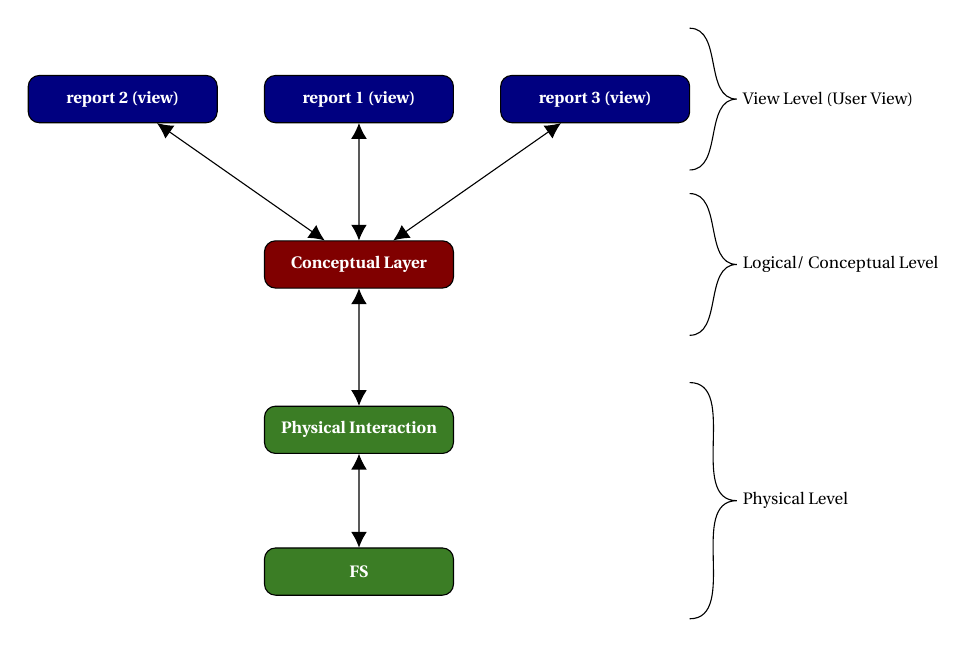
\begin{tikzpicture}[node distance=2cm,
					every node/.style={fill=white, font=\sffamily}, align=center,
					scale=0.6, 
					every node/.style={transform shape}]

% Specification of nodes (position, etc.)
\node (view2)             [optionalETL]              {report 2 (view)};
\node (view1)     [optionalETL, right of=view2, xshift=3cm]          {report 1 (view)};
\node (view3)      [optionalETL, right of=view1, xshift=3cm]   {report 3 (view)};
\node (concept)     [required,below of=view1, yshift=-1.5cm]   {Conceptual Layer};
\node (physical)      [optionalELK, below of=concept, yshift=-1.5cm] {Physical Interaction};
\node (fs)      [optionalELK, below of=physical, yshift=-1cm] {FS};

%\node (Appendix) [startstop, above of=Arch] {Ch.13 Appendix};     
% Normal Path
\draw[<->]     (view2) -- (concept);
\draw[<->]     (view3) -- (concept);
\draw[<->]     (view1) -- (concept);
\draw[<->]     (concept) -- (physical);
\draw[<->]     (fs) -- (physical);
\draw[-]      (12,-1.5) to[out=0,in=180] (13,0)  node[right]{View Level (User View) } to[out=180,in=0] (12,1.5);
\draw[-]      (12,-5) to[out=0,in=180] (13,-3.5) node[right]{Logical/ Conceptual Level } to[out=180,in=0]  (12,-2);
\draw[-]      (12,-11) to[out=0,in=180] (13,-8.5) node[right]{Physical Level } to[out=180,in=0]  (12,-6);
\end{tikzpicture}
}

%%%%%%%%%%%%%%%%%%%%%%%%%%%%%%%%%%%%%%%%%%%%%%%%%%%%%%%%%%%%%%%%%%%%%%%%%%%
%%% Local Variables:
%%% mode: latex
%%% TeX-master: "../../main.tex"
% !TeX root = ../../main.tex
%%% TeX-engine: xetex
%%% End:

\end{frame}
%---------------------------------------------------------
\VideoClassification
%%%%%%%%%%%%%%%%%%%%%%%%%%%%%%%%%%%%%%%%%%%%%%%%%%%%%%
\begin{frame}
	\frametitle{Physical level}
	\begin{itemize}[<+->]
		\item \textbf{Physical level (Internal)}: 
		\begin{itemize}[<+->]
			\item Lowest level.
			\item Describes \textbf{\underline{\blue{how}}} data is stored.
			\item Describes the data structure.
			\item It allows you to modify the lowest level (Physical part) without any change in the logical schema. These change could be
				\begin{itemize}[<+->]				
					\item Using a new storage device
					\item Change the structure of the data used for storage
					\item Change the file type or use a different storage structure
					\item Chang the access method
					\item Modify indexes
					\item Change the compression algorithm or hashing technique.
			\end{itemize}									
		\end{itemize}		
		%https://beginnersbook.com/2015/04/levels-of-abstraction-in-dbms/		
		%https://www.guru99.com/dbms-data-independence.html
	\end{itemize}	
\end{frame}
%%%%%%%%%%%%%%%%%%%%%%%%%%%%%%%%%%%%%%%%%%%%%%%%%%%%%%
\begin{frame}
	\frametitle{Physical level}
	\begin{example}		
		\begin{itemize}[<+->]
			\item Database contains product information.
			\item Physical layer describes
			\begin{itemize}[<+->]
				\item Storage mechanism and the blocks (bytes, gigabytes, terabytes, etc.).
				\item The amount of memory used.
				\item Usually this layer abstracted from the programmers.
			\end{itemize}
		\end{itemize}
	\end{example}
	
\end{frame}
%---------------------------------------------------------
%---------------------------------------------------------
\VideoClassification
%%%%%%%%%%%%%%%%%%%%%%%%%%%%%%%%%%%%%%%%%%%%%%%%%%%%%%
\begin{frame}
	\frametitle{Logical level}
	\begin{itemize}[<+->]
		\item \textbf{Logical level (Conceptual)}: 
		\begin{itemize}[<+->]
			\item Intermediate level
			\item Describes \textbf{\underline{\blue{what}}} data is stored
			\item Describes what the relationship between the stored data is?
			\item It allows you to change the logical view without altering the external view, API, or programs. These change could be
			\begin{itemize}[<+->]
				\item Add a new table
				\item Change the records merge or delete without affecting the running applications
				\item Change attribute (Add,delete) to the existing table
			\end{itemize}									
		\end{itemize}		
	\end{itemize}	 
\end{frame}
%%%%%%%%%%%%%%%%%%%%%%%%%%%%%%%%%%%%%%%%%%%%%%%%%%%%%%
\begin{frame}
	\frametitle{Logical level}
	\begin{example}
		\begin{itemize}[<+->]
			\item Database contains product information.
			\item Logical Layer describes
			\begin{itemize}[<+->]
				\item The product fields and their data types
				\item How this product interact with other entities in the database
				\item The programmers' design this level based on business knowledge and the requirements
			\end{itemize}
		\end{itemize}
	\end{example}
	
\end{frame}


%---------------------------------------------------------
%---------------------------------------------------------
\VideoClassification
%%%%%%%%%%%%%%%%%%%%%%%%%%%%%%%%%%%%%%%%%%%%%%%%%%%%%
\begin{frame}
	\frametitle{View level}
	\begin{itemize}
		\item \textbf{View level (External)}: 
		\begin{itemize}
			\item Highest level.
			\item \textbf{\underline{\blue{View}}} of the data stored? 
			\item Designed for a category of users
			\item The final interface for the user
			\item Extended or hidden based on the user's role
			\item Not all the views is extended to all users, and there is authentication based on the category
		\end{itemize}		
	\end{itemize}	
	
\end{frame}
%%%%%%%%%%%%%%%%%%%%%%%%%%%%%%%%%%%%%%%%%%%%%%%%%%%%%
\begin{frame}
	\frametitle{View level}
	\begin{example}
		\begin{itemize}
			\item The database contains product information
			\item It could be designed to show the sales of the product in a specific region
			\item We might hide information about some products based on the teams or users
		\end{itemize}
	\end{example}
	
\end{frame}

%---------------------------------------------------------
%---------------------------------------------------------
\VideoClassification[column=2, colour=blue]
%%%%%%%%%%%%%%%%%%%%%%%%%%%%%%%%%%%%%%%%%%%%%%%%%%%%%%
\begin{frame}[c]
	\frametitle{Data solution thinking (Summary) }
	% !!!!!!!!!!!!!! We need to mention that this slide is just an overview there will be a detailed one later
        \begin{center}
			Let's answer our previous question. How can we solve data challenges?
        \end{center}
    \end{frame}

%%%%%%%%%%%%%%%%%%%%%%%%%%%%%%%%%%%%%%%%%%%%%%%%%%%%%%

%%%%%%%%%%%%%%%%%%%%%%%%%%%%%%%%%%%%%%%%%%%%%%%%%%%%%% 
\begin{frame}
	\frametitle{Data solution thinking (Summary) }
	\begin{itemize}[<+->]
        \item Let's split the problem based on the data layers.
          \begin{itemize}[<+->]
          \item View layer
            \begin{itemize}[<+->]
            \item When we need to add/remove/create new reports, it is usually a view layer.
            \item We don't need to change the logical or physical layer to support the view layer.
          \end{itemize}
        \end{itemize}
       \end{itemize}
 \end{frame}

%%%%%%%%%%%%%%%%%%%%%%%%%%%%%%%%%%%%%%%%%%%%%%%%%%%%%% 
\begin{frame}
\frametitle{Data solution thinking (Summary) }
	\begin{itemize}[<+->]
        \item Let's split the problem based on the data layers.
          \begin{itemize}[<+->]
           \item Logical Layer
           \begin{itemize}[<+->]
             \item When you have missing sources into your logical layer, and you need to add this source and its structure.
             \item There is a performance issue in the existing reports, and you need to change the model. \forexample reduce the join by creating a new join table (\textit{materialized view}).
             \item Update the data type or the existing relation, which could help to fix some data or performance issues.
            \end{itemize}
           \end{itemize}
        \end{itemize}
 \end{frame}

 %%%%%%%%%%%%%%%%%%%%%%%%%%%%%%%%%%%%%%%%%%%%%%%%%%%%%%%
 %%%%%%%%%%%%%%%%%%%%%%%%%%%%%%%%%%%%%%%%%%%%%%%%%%%%%% 
\begin{frame}
  \frametitle{Data solution thinking (Summary) }
  \begin{itemize}[<+->]
  \item Let's split the problem based on the data layers.
    \begin{itemize}[<+->]
    \item Physical Layer
      \begin{itemize}[<+->]
      \item When our problem is hard or impossible to fix by optimizing the query (view)/ logical layer, it is time for physical change.
      \item If we need to change your storage/compression/structure/access technique.
      \item If we need to change the data orientation structure from row to column or key-value storage, It is time to change the physical layer.
      \end{itemize}
    \end{itemize}
  \end{itemize}
 \end{frame}






%%%%%%%%%%%%%%%%%%%%%%%%%%%%%%%%%%%%%%%%%%%%%%%%%%%%%%%%%%%%%%%%%%%%%%%%%%%%
%%% Local Variables:
%%% mode: latex
%%% TeX-master: "../main"
% !TeX root = ../main.tex
%%% TeX-engine: xetex
%%% End:
%-------------------------------------------------------%
%---------------------------------------------------------
\VideoClassification[column=2, colour=blue]
%%%%%%%%%%%%%%%%%%%%%%%%%%%%%%%%%%%%%%%%%%%%%%%%%%%%%%%
\subsection{Introduction to DWH}

\subsubsection{Motivation to the Data Warehouse (DWH)}
\begin{frame}
\frametitle{Motivation to the Data Warehouse (DWH)}
	\begin{itemize}[<+->]
		\item Data could be a product for some companies.
		\item It could be decision support for other products or businesses.
		\item It could be reporting the results after passing the data life-cycle from storage (Database).
		\item Some challenges are facing the people who work on data management backend:
			\begin{itemize}[<+->]
				\item Performance,
				\item Integration,
				\item and Applying analytical functions. %Moving average
			\end{itemize}
		\item Vendors who are working on solving the above challenges are creating their product of DWH. Their ultimate goal is to optimize the above points.
	\end{itemize}
\end{frame}
%%%%%%%%%%%%%%%%%%%%%%%%%%%%%%%%%%%%%%%%%%%%%%%%%%%%%%
\begin{frame}[c]
\frametitle{Motivation to the Data Warehouse (DWH)}

\begin{definition}[What is Data Warehousing?] A DWH is a technique for collecting and managing data from varied sources to \textbf{provide meaningful business insights}. It is a blend of technologies and components which aids the strategic use of data.%\footnotemark
\end{definition}

%REF
Inmon Bill gave the real concept. He is considered the father of the DWH. He had written about a variety of topics for building, usage, and maintenance of the warehouse \& the Corporate Information Factory

%\footnotetext{The definition mentioned in this slides copied from  \href{https://www.guru99.com/data-warehousing.html\#2}{guru99.com} }

\end{frame}

%%%%%%%%%%%%%%%%%%%%%%%%%%%%%%%%%%%%%%%%%%%%%%%%%%%%%%

%%%%%%%%%%%%%%%%%%%%%%%%%%%%%%%%%%%%%%%%%%%%%%%%%%%%%%
\begin{frame}
\frametitle{Motivation to the Data Warehouse (DWH)}

\begin{itemize}[<+->]
	\item The DWH is not a product but an environment.
	\item It is a process of transforming data into information and make it available to users in a \textbf{timely manner} to make a difference.
	\item It is an architectural construct of an information system that provides users with current and historical decision support information which is difficult to access or present in the traditional operational data store.
	\item The DWH is the core of the BI system built for data analysis and reporting.
\end{itemize}

\end{frame}

%%%%%%%%%%%%%%%%%%%%%%%%%%%%%%%%%%%%%%%%%%%%%%%%%%%%%%

\begin{frame}
\frametitle{Motivation to the Data Warehouse}

Other names for the Data warehouse system:

\begin{wideitemize}
\item Decision Support System (DSS).
\item Business Intelligence Solution.
\item Executive Information System.
\item Management Information System.
\item Analytic Application.
\item Data Warehouse.

\end{wideitemize}


\end{frame}

%-------------------------------------------------------%
%---------------------------------------------------------
\VideoClassification[column=2]
%%%%%%%%%%%%%%%%%%%%%%%%%%%%%%%%%%%%%%%%%%%%%%%%%%%%%%
\subsubsection{Differences Between DWH and Operational DB}
\begin{frame}
	\frametitle{DWH vs Operational databases}

	\begin{table}[t]
		\centering	
		\resizebox{\columnwidth}{!}{%
			
			%		\centering
			\begin{tabular}{|c | c | c|}
				\hline
				\textbf{Metric}  & \textbf{Transactions DB}& \textbf{DWH} \\
				\hline
				Volume & GB/TB & TB/PB \\
				Historical  & Short-term & Long-Term\\
				rows & <1000M &  1000M>\\
				Orientation & Product & Subject or multi products\\
				Business Units & Product team & Multi organizational units\\
				Normalization & Normalized %due to storage and performance limitation and its design
				&  Not required (De-normalized in many use cases)\\
				Data Model & Relational & Star Schema or Multi-dim\\
				Intelligence&Reporting & Advanced reporting and Machine Learning\\
				Use cases& Online transactions \& operations & Centeralized storage (360\textdegree)\\
				\hline
			\end{tabular}
			%		\caption{Data Representation Combination Matrix}\label{Tab:Data_Representation_Matrix}
		}
	\end{table}
\end{frame}

%---------------------------------------------------------
\VideoClassification[column=2, colour=blue]
%%%%%%%%%%%%%%%%%%%%%%%%%%%%%%%%%%%%%%%%%%%%%%%%%%%%%%

\begin{frame}
\frametitle{Transactional DB Use cases}
\begin{figure}[ht]
	
	\centering
	\includegraphics[width=\linewidth]{./Figures/chapter-01/baby-01.jpg}
	%		\includegraphics[width=\linewidth,height=\textheight]{./Figures/chapter-01/baby-02.jpg}
	%	\caption{}
\end{figure}
\end{frame}


%%%%%%%%%%%%%%%%%%%%%%%%%%%%%%%%%%%%%%%%%%%%%%%%%%%%%%
\begin{frame}
\frametitle{Transactional DB Use cases}
\begin{figure}[ht]

\centering
%	\includegraphics[width=\linewidth]{./Figures/chapter-01/baby-01.jpg}
\includegraphics[width=\linewidth]{./Figures/chapter-01/baby-02.jpg}
%	\caption{}
\end{figure}
\end{frame}


%%%%%%%%%%%%%%%%%%%%%%%%%%%%%%%%%%%%%%%%%%%%%%%%%%%%%%
\begin{frame}
\frametitle{DWH Use cases}
\begin{figure}[ht]

\centering
\includegraphics[width=\linewidth,height=.8\textheight]{./Figures/chapter-01/Marvel-03.jpg}
%	\caption{}
\end{figure}
\end{frame}

%%%%%%%%%%%%%%%%%%%%%%%%%%%%%%%%%%%%%%%%%%%%%%%%%%%%%%
\begin{frame}
\frametitle{DWH Use cases}
\begin{figure}[ht]

\centering
\includegraphics[width=\linewidth,height=.8\textheight]{./Figures/chapter-01/Marvel-02.jpg}
%	\caption{}
\end{figure}
\end{frame}

%%%%%%%%%%%%%%%%%%%%%%%%%%%%%%%%%%%%%%%%%%%%%%%%%%%%%%
\begin{frame}
\frametitle{DWH Use cases}
\begin{figure}[ht]

\centering
\includegraphics[width=\linewidth,height=.8\textheight]{./Figures/chapter-01/Marvel-01.jpg}
%	\caption{}
\end{figure}
\end{frame}





%%%%%%%%%%%%%%%%%%%%%%%%%%%%%%%%%%%%%%%%%%%%%%%%%%%%%%%%%%%%%%%%%%%%%%%%%%%%
%%% Local Variables:
%%% mode: latex
%%% TeX-master: "../main"
% !TeX root = ../main.tex
%%% TeX-engine: xetex
%%% End:
%-------------------------------------------------------%
%---------------------------------------------------------
\VideoClassification[column=2, colour=blue]
%%%%%%%%%%%%%%%%%%%%%%%%%%%%%%%%%%%%%%%%%%%%%%%%%%%%%%
\subsubsection{Types of DWH}
\begin{frame}
\frametitle{Motivation to Data Warehouse}
Types of Data Warehouse
\begin{description}
\item [\textbf{Enterprise Data Warehouse (EDWH)}] It provides decision support service across the enterprise. It offers a unified approach for organizing and representing data (DWH Model). It offers data classifications according to the subject with privileges policy.
\item [\textbf{Operational Data Store (ODS):}] is a central database that provides an up-to-date (real-time) data from multiple transnational systems for operational reporting into a single DWH.

%% for real time questions and answers. call ODS using intermidiate data store. DWH is day -1 (billing & subscribtions). Oracle (Loading or headache) && CDC capture change interest column not row
\item [\textbf{Data Mart:}] A data mart is a subset of the data warehouse. It specially designed for a particular line of business, such as sales, finance, sales or finance. In an independent data mart, data can collect directly from sources.
\end{description}

\end{frame}

%%%%%%%%%%%%%%%%%%%%%%%%%%%%%%%%%%%%%%%%%%%%%%%%%%%%%%

\begin{frame}
\frametitle{DWH vs ODS vs Data Mart}


\begin{table}[t]
\centering	
\resizebox{\columnwidth}{!}{%

%		\centering
\begin{tabular}{|c | c | c| c |}
\hline
\textbf{Metric}  & \textbf{DWH}& \textbf{ODS} & \textbf{Data Mart} \\
\hline
Latency & Day -1  & Real-time & Day -1 \\			
Data level  & Transnational & Transnational & Summary \\
Historical  & Long-term & Snapshot & Aggregated Long-Term \\
Size & TB/PB & GB & GB/TB\\
Orientation & Multi sources & Multi sources & Product\\
Business Units & Multi organizational units & Product team & Business team \\
\hline
\end{tabular}
%		\caption{Data Representation Combination Matrix}\label{Tab:Data_Representation_Matrix}
}
\end{table}
\end{frame}

%-------------------------------------------------------%

%%%%%%%%%%%%%%%%%%%%%%%%%%%%%%%%%%%%%%%%%%%%%%%%%%%%%%%%%%%%%%%%%%%%%%%%
\subsubsection{Use Cases of Operational DB vs DWH}

\begin{frame}
\frametitle{Use case (Operational DB)}

\begin{itemize}[<+->]

\item A telecommunication company named \textbf{XTec}.
\newline
\item They have lots of systems. One of this systems is a CRM system as example of operational DB.
\begin{itemize}[<+->]

\item The CRM system handles the customer activities with the company including (sales, change in customer plans, and other activities).
\item This system has a backend database (MySQL).
\item CRM team can report their sales and customer activities from their database.
\item Product owner can take a decision based on their system backend reports.

\end{itemize}

\end{itemize}

\end{frame}

%%%%%%%%%%%%%%%%%%%%%%%%%%%%%%%%%%%%%%%%%%%%%%%%%%%%%%

\begin{frame}
\frametitle{Use case (DWH)}

\begin{itemize}[<+->]

\item What is the need for DWH?		
\begin{itemize}[<+->]
\item This company has other systems \forexample billing, charging, signaling.	
\item They need to report information related to the CRM, billing, and signaling source systems in one report.
\item So, they need to ingest (transfer) the data from the source systems to one single database.
\item The decision from the DHW is a \textbf{global and strategical decision.}
\item If the company needs to build a machine learning model which needs data from different sources. They need to load the data from a centralized database rather than read each source alone.
\end{itemize}

\end{itemize}

\end{frame}
%%%%%%%%%%%%%%%%%%%%%%%%%%%%%%%%%%%%%%%%%%%%%%%%%%%%%%


\begin{frame}
\frametitle{Use case (DWH)}
\centering
The Full picture required a DWH. However, we still need the other operational databases for product development perspective.


\end{frame}
%%%%%%%%%%%%%%%%%%%%%%%%%%%%%%%%%%%%%%%%%%%%%%%%%%%%%%

\begin{frame}
\frametitle{Use case (ODS)}
\centering

\begin{itemize}[<+->]
\item Why do we need the ODS?
\item 	How does it fit in our system?
\end{itemize}


\end{frame}
%%%%%%%%%%%%%%%%%%%%%%%%%%%%%%%%%%%%%%%%%%%%%%%%%%%%%%


%%%%%%%%%%%%%%%%%%%%%%%%%%%%%%%%%%%%%%%%%%%%%%%%%%%%%%

\begin{frame}
\frametitle{Use case (ODS)}
\centering
\textbf{XTec} has a call center system which handles the customer inquiries. This system requires the some data related to usage, customer information, billing details to be calculated and accumulated in \textbf{real-time} to be able to give the customer the right answer for his inquires.

\end{frame}
%%%%%%%%%%%%%%%%%%%%%%%%%%%%%%%%%%%%%%%%%%%%%%%%%%%%%%
%%%%%%%%%%%%%%%%%%%%%%%%%%%%%%%%%%%%%%%%%%%%%%%%%%%%%%
\begin{frame}
\frametitle{Use case (ODS)}

	\begin{itemize}[<+->]
		\item So, What is the challenge for this system?
			\begin{itemize}[<+->]		
				\item It needs specific information from different source systems.
				\item It requires to track the source system database changes or update in real-time.
				\item It's functionality is based on the aggregate data not the transactions \forexample (It needs the total outgoing calls till time or it needs the total charging amounts from prepaid or the available limits from billing if it is postpaid).
			\end{itemize}
	\end{itemize}

\end{frame}
%%%%%%%%%%%%%%%%%%%%%%%%%%%%%%%%%%%%%%%%%%%%%%%%%%%%%%
\begin{frame}
\frametitle{Use case (ODS)}

	\begin{itemize}[<+->]
		\item ODS is based on change data capture (CDC). This approach used to determine the data change and apply action based on this change.
		\item ODS uses the real-time aggregations to support the online systems from different source systems.
	\end{itemize}
\end{frame}






%%%%%%%%%%%%%%%%%%%%%%%%%%%%%%%%%%%%%%%%%%%%%%%%%%%%%%%%%%%%%%%%%%%%%%%%%%%%
%%% Local Variables:
%%% mode: latex
%%% TeX-master: "../main"
% !TeX root = ../main.tex
%%% TeX-engine: xetex
%%% End:
%-------------------------------------------------------%

%---------------------------------------------------------
\VideoClassification[column=2, colour=red]
%%%%%%%%%%%%%%%%%%%%%%%%%%%%%%%%%%%%%%%%%%%%%%%%%%%%%%

\subsection{Hot vs Cold Storage}
\begin{frame}[c]
\frametitle{Hot vs Cold Storage}

%\begin{center}
\includegraphics[width=\textheight]{./Figures/chapter-01/WWH-Thumb.png}

%\end{center}


\end{frame}
%%%%%%%%%%%%%%%%%%%%%%%%%%%%%%%%%%%%%%%%%%%%%%%%%%%%%%


\begin{frame}
\frametitle{What is multi-temperature Storage?}

\begin{wideitemize}
\item (Most of) DWH solution design has multi-temperature data management model.
\item What is the multi-temperature data management model?
\begin{itemize}[<+->]
	\item It is a data classification design which allows us to have the following characteristics
	\begin{itemize}[<+->]
		\item  (high performance) access on the frequent data (Hot data).
		\item Good (average performance) access to less-frequently data (warm data).
		\item Availability to access rarely accessed data (cold data).
	\end{itemize}
	\item Who is responsible for data temperature classifications?
	\begin{itemize}[<+->]
		\item Demand team, product owner, or data architect (Based on the business needs).
	\end{itemize}
\end{itemize}
\end{wideitemize}
\end{frame}

%%%%%%%%%%%%%%%%%%%%%%%%%%%%%%%%%%%%%%%%%%%%%%%%%%%%%%

\begin{frame}
\frametitle{Why do we need it?}

\begin{wideitemize}
\item Why do we need the multi-temperature data management model?
\begin{itemize}[<+->]
\item Cost reduction \blue{\faDollar \faDollar \faDollar \faDollar}
\item Performance.
\end{itemize}
\end{wideitemize}
\end{frame}
%%%%%%%%%%%%%%%%%%%%%%%%%%%%%%%%%%%%%%%%%%%%%%%%%%%%%%

\begin{frame}
\frametitle{How to implement a multi-temperature storage system? }

\begin{wideitemize}
\item How to implement the multi-temperature data management model?
\begin{itemize}[<+->]
\item Before implementation, we need to know the following:
\begin{itemize}[<+->]
\item Frequency of access
\item Data change rate.
\end{itemize}
\item Identify which storage type is suitable for the project
\begin{itemize}[<+->]
\item We store the hot data on the fast storage system.
\item Warm data (usual) stored on slightly slower storage.
\item We store the cold data on the slowest storage.
\end{itemize}
\end{itemize}
\end{wideitemize}
\end{frame}

%%%%%%%%%%%%%%%%%%%%%%%%%%%%%%%%%%%%%%%%%%%%%%%%%%%%%%

\begin{frame}
\frametitle{How to implement a multi-temperature storage system? Cont.}

\begin{wideitemize}
\item Design consideration to make the retention easily.
\begin{itemize}[<+->]
\item Table partitions need to be split based on the retention policy plan \forexample (date).
\item Summary tables (agg) need to be maintained to reduce the need for access the cold storage.
\item Backup, Recovery, and Rollback plans need to be automated and prepared/tested before moving the data.
\end{itemize}
\end{wideitemize}
\end{frame}

%%%%%%%%%%%%%%%%%%%%%%%%%%%%%%%%%%%%%%%%%%%%%%%%%%%%%%

%%%%%%%%%%%%%%%%%%%%%%%%%%%%%%%%%%%%%%%%%%%%%%%%%%%%%%

\begin{frame}
\frametitle{How to implement a multi-temperature storage system? Cont.}
\begin{wideitemize}
\item Implementation (summary):
\begin{itemize}[<+->]
\item There are lots of tools for this purpose and  categorized as follows:
\begin{itemize}
\item Enterprise.
\item Open source.
\item Cloud tools.
\end{itemize}

\end{itemize}
%Cost,Security
\end{wideitemize}
\end{frame}
%%%%%%%%%%%%%%%%%%%%%%%%%%%%%%%%%%%%%%%%%%%%%%%%%%%%%%

\begin{frame}
\frametitle{How to implement a multi-temperature storage system? Cont.}
\begin{wideitemize}
\item Enterprise \forexample:
\begin{itemize}
\item IBM InfoSphere
\item Informatica PowerCenter
\item Oracle Data Service Integrator
\item Talend Data Integration
\item Microsoft SQL
\end{itemize}
%Cost,Security
\end{wideitemize}
\end{frame}

%%%%%%%%%%%%%%%%%%%%%%%%%%%%%%%%%%%%%%%%%%%%%%%%%%%%%%

\begin{frame}
\frametitle{How to implement a multi-temperature storage system? Cont.}
\begin{wideitemize}
\item Open source \forexample:
\begin{itemize}
\item Apache NiFi*
\item CloverETL
\item Pentaho
\item Talend Open Studio*
\end{itemize}
\end{wideitemize}
\end{frame}

%%%%%%%%%%%%%%%%%%%%%%%%%%%%%%%%%%%%%%%%%%%%%%%%%%%%%%

\begin{frame}
\frametitle{How to implement a multi-temperature storage system? Cont.}
\begin{wideitemize}
\item Cloud tools \forexample:
\begin{itemize}
\item AWS Migration Services.
\item Azure Migration Tools.
\item Google Migration Services/Velostrata.
\end{itemize}
\item Some cloud providers offer physical data movement services.
\item How to choose the most suitable storage type for your project/organization?
%Cost,Security
\end{wideitemize}
\end{frame}





%%%%%%%%%%%%%%%%%%%%%%%%%%%%%%%%%%%%%%%%%%%%%%%%%%%%%%%%%%%%%%%%%%%%%%%%%%%%
%%% Local Variables:
%%% mode: latex
%%% TeX-master: "../main"
% !TeX root = ../main.tex
%%% TeX-engine: xetex
%%% End:
%-------------------------------------------------------%

%---------------------------------------------------------
\VideoClassification[column=2, colour=red]
%%%%%%%%%%%%%%%%%%%%%%%%%%%%%%%%%%%%%%%%%%%%%%%%%%%%%%
\subsection{DWH Characteristics}
\begin{frame}
    \frametitle{DWH Characteristics}
    %these is not a definitions, we just show the meaning and the understanding.
    \begin{wideitemize}
        \item The characteristics of DWH:
        \begin{wideitemize}
        	\item Integrated: \textit{DWH is an integrated environment which allows us to
        	integrate different source systems. Data are modeled (organized) in a unified manner}.%regardless of the original source
        	
        	\item Time-Variant: \textit{Data modeled (organized) based on periods
        	(hourly, daily, weekly, monthly, quarterly, yearly)}.
        	
        	\item Subject-oriented: \textit{DWH main target is to support business needs for
        	the whole organization including (decision-makers, departments, and
        	specific user requirements)}.
        	
        	\item Non-Volatile: \textit{It refers to the data that erased or deleted (It could be archived and retrieved when needed). Data can be accumulated daily the new snapshots (refreshed at based on the source system interval.  \faArrowCircleORight \space It could be updated daily, weekly, and monthly)}.
        \end{wideitemize}
    \end{wideitemize}
\end{frame}
%%%%%%%%%%%%%%%%%%%%%%%%%%%%%%%%%%%%%%%%%%%%%%%%%%%%%%
\subsection{DWH Architecture}
\begin{frame}
\frametitle{DWH Architecture Overview}
	\begin{tikzpicture}[every label/.append style={font=\tiny},regentonne/.style={cylinder,aspect=.7,draw,shape border rotate=90}]
		%\draw[step=.5cm,gray,very thin] (-2,-1) grid (9.5,6);
		%SS recatangle
		\filldraw[draw=blue,thick,rounded corners,fill=white] (-2,-1) rectangle (0.2,6);

		%ETL recatangle		
		\filldraw[draw=Maroon,thick,rounded corners,fill=white] (.4,0) rectangle (2.5,6);
		
		%EDW
		\filldraw[draw=OliveGreen,thick,rounded corners,fill=white] (2.7,0) rectangle (7.7,6);
		
		%BI LAYER
		\filldraw[draw=mauve,thick,rounded corners,fill=white] (7.9,0) rectangle (9.5,6);

		%Metadata LAYER
		\filldraw[draw=ballblue,thick,rounded corners,fill=white] (.4,-1.2) rectangle (9.5,-.7);

		%User Access LAYER
		\filldraw[draw=black,thick,rounded corners,fill=white] (.4,-.6) rectangle (9.5,-.1);

		
   	    \node[text width=2cm,font=\scriptsize] at (-.9,5.6) {Source Systems};
		\node[database,label=below:CRM] (s1) at (-1,5) {};
		\node[database,label=below:ERP] (s2) at (-1,4) {};
		\node[database,label=below:MobileApp] (s3) at (-1,3) {};		
		\node[database,label=below:Billing] (s4) at (-1,2) {};		
		\node[database,label=below:WebApp] (s5) at (-1,1) {};						
		\node[database,label=below:Other] (s6) at (-1,0) {};				
		
		\draw[line width=0.25mm, blue] (s1) -- ([xshift=.5cm]s1.east) -- ([xshift=.5cm]s2.east) -- (s2)  -- ([xshift=.5cm]s2.east) -- ([xshift=.5cm]s3.east) -- (s3)-- ([xshift=.5cm]s3.east) -- ([xshift=.5cm]s4.east) -- (s4) -- ([xshift=.5cm]s4.east) --  ([xshift=.5cm]s5.east) -- (s5) --  ([xshift=.5cm]s5.east) -- ([xshift=.5cm]s6.east) -- (s6);
	
		%connection arrow
		\draw[->,line width=0.5mm, black] ([xshift=.5cm,yshift=-.5cm]s3.east) -- ([xshift=1.45cm,yshift=-.5cm]s3.east) ;		

		
		%ETL
   	    \node[text width=2cm,font=\scriptsize] at (2.2,5.6) {ETL};
        \pic[draw,fill=Maroon]          (etlS) at (1.45,4.3)   {gear={0.08}{17}{15}};
        \pic[draw,fill=uiborange]       (etlM) at (1.45,2.5)   {gear={0.08}{17}{15}};
        \pic[draw,fill=mygreen]         (etlB) at (1.45,.8)   {gear={0.08}{17}{15}};
   		\draw[line width=0.25mm, gray] (2.03,4.3) -- (2.4,4.3);
  		\draw[line width=0.25mm, gray] (2.03,2.5) -- (2.4,2.5);
  		\draw[line width=0.25mm, gray] (2.03,.8) -- (2.4,0.8);
  		\draw[line width=0.25mm, gray] (2.4,4.3) -- (2.4,0.8);  		
		%connection arrow	
  		\draw[->,line width=0.5mm, black] (2.4,2.5) -- (3.3,2.5);
   		
		%EDW
   	    \node[text width=4.5cm,font=\scriptsize] at (5.3,5.6) {Enterprise Data Warehouse (EDW)};
     	\node[database,label=below:DWH,database radius=.7cm,database segment height=.4cm] (A)  at (4,2.6) {};
     	\node[database,label=below:Data Mart,database radius=.4cm,database segment height=.2cm]  (B)  at (6.5,4) {};     	
     	\node[database,label=below:Data Mart,database radius=.4cm,database segment height=.2cm]  (C)  at (6.5,2.5) {};
     	\node[database,label=below:Data Mart,database radius=.4cm,database segment height=.2cm]  (D)  at (6.5,1) {};     	
     	\node[database,label=below:Operational Data Store,database radius=.6cm,database segment height=.3cm] (E) at (4,4.6) {};
    
       \draw[line width=0.25mm,alizarin,->] (A) -- (B);
       \draw[line width=0.25mm,alizarin,->] (A) -- (C);
       \draw[line width=0.25mm,alizarin,->] (A) -- (D);
       \draw[line width=0.25mm,alizarin,->] (E) -- (A);

       \draw[line width=0.25mm,alizarin] (7.3,.9) -- (7.3,4);
       
       \draw[line width=0.25mm,alizarin] (6.9,4) -- (7.3,4);
       \draw[line width=0.25mm,alizarin] (6.9,2.5) -- (7.3,2.5);
       \draw[line width=0.25mm,alizarin] (6.9,.9) -- (7.3,.9);
       
       \draw[line width=0.5mm,black,->] (7.3,2.5) -- (8,2.5);
       
		%BI LAYER
		\node[text width=1.3cm,font=\scriptsize] at (8.8,5.6) {BI Layer};
		\node[inner sep=0pt] (rep) at (8.7,4.6) {\includegraphics[width=.1\textwidth,height=.1\textheight]{./Figures/chapter-01/report.png}};
		\node[yshift=.4cm,below of=rep] {{\tiny Reporting}};
		\node (io) at (8.7,2.5) [io] {{\tiny Analytics}}; 		
		\node (start) at (8.7,0.5) [startstop] {{\tiny Integrations}}; 

		%MDM
		\node at (4.5,-.4) {Metadata Repository Management (MDM)};
		
		%Access Layer
		\node at (4.5,-1) {User Access Management \faExpeditedssl};
		
	\end{tikzpicture}

\end{frame}
%%%%%%%%%%%%%%%%%%%%%%%%%%%%%%%%%%%%%%%%%%%%%%%%%%%%%%
\begin{frame}
\frametitle{DWH Architecture Layers}

\begin{wideitemize}
	\item DWH architecture contains the following layers:
	\begin{itemize}[<+->]
		\item Source system layer.
		\item Extraction layer.
		\item Staging Area.
		\item Data Modeling.
		\item ETL layer.
		\item Storage layer.
		\item Reporting (UI) layer.
		\item Metadata layer.
		\item System operations layer.
	\end{itemize}
\end{wideitemize}

\end{frame}
\VideoClassification[column=2, colour=blue]




%%%%%%%%%%%%%%%%%%%%%%%%%%%%%%%%%%%%%%%%%%%%%%%%%%%%%%%%%%%%%%%%%%%%%%%%%%%%
%%% Local Variables:
%%% mode: latex
%%% TeX-master: "../main"
% !TeX root = ../main.tex
%%% TeX-engine: xetex
%%% End:
%-------------------------------------------------------%
%%%%%%%%%%%%%%%%%%%%%%%%%%%%%%%%%%%%%%%%%%%%%%%%%%%%%%
\subsubsection{Source System Integration Process}
\begin{frame}
    \frametitle{Source System Integration Process}
    \begin{itemize}[<+->]
        \item In some companies, they hire or dedicate a team for this part (business analyst, system analyst, data analyst, or demand team).
        \item Before we start, we need to document all the communications into any format.
		\begin{itemize}
            \item Confluence pages, Word, or Excel sheet.
            \item Make the discussion online and put comments to make the history available always.
			\item We need to clarify all the tasks and what is the expected output, \forexample (analysis means to document data structure, format, column names, etc.).
        \end{itemize}
    \end{itemize}

\end{frame}

%%%%%%%%%%%%%%%%%%%%%%%%%%%%%%%%%%%%%%%%%%%%%%%%%%%%%%
\begin{frame}
    \frametitle{Source System Integration Process}
    \begin{itemize}[<+->]
        \item  Requirements gathering. % or business need (It could be DWH unification).
        \item  Identify the stakeholders (Data owner(s)).
        \item  Data Analysis includes but not only (format, latency, and column definitions).
        \item  Check the source system access and perform connectivity assessment.
        \item  Initiate the technical discussion about the best way to ingest the data.
        \item  Data Ingestion method and format.
        \item  Sign or confirmation for every point between the stakeholders.
        \item  \blue{This layer deliver a data analysis (Source system interface ) document}.
    \end{itemize}

\end{frame}

%-------------------------------------------------------%
%%%%%%%%%%%%%%%%%%%%%%%%%%%%%%%%%%%%%%%%%%%%%%%%%%%%%%
\VideoClassification[column=2, colour=blue]
\subsubsection{Extraction Layer}

\begin{frame}
    \frametitle{Extraction Layer}
    \begin{itemize}[<+->]
		\item In some companies, they hire or dedicate a team for this part (extraction or ingestion team), but in other companies, it is part of the data engineering team.
		\item This layer takes the output analysis and decisions from the previous layer (source system analysis) and implement the extraction (quality from the previous team output highly affect this team).
		\item There is a lot of consideration this team needs to take care of or deal with, but we can summarize it in the following:
		\begin{itemize}[<+->]
			\item Data latency analysis as it affects the tool and the methodology (stream or batch).
			\item Data extraction method (push or pull).
			\item Data size and format compared with the available resources for this project.
	    \end{itemize}
        \item \blue{This layer output is a minimal data cleansing (no transformation) into the staging/landing layer}.
    \end{itemize}
\end{frame}

%-------------------------------------------------------%
%%%%%%%%%%%%%%%%%%%%%%%%%%%%%%%%%%%%%%%%%%%%%%%%%%%%%

\subsubsection{Staging Layer}
\begin{frame}
    \frametitle{Staging Layer}
    \begin{itemize}[<+->]
        \item This layer handled by the same team who own the \blue{storage part} in most of the organizations.
        \item Segregation of this layer if it uses different storage type or multi-teams access this layer for a different purpose \forexample (Kafka)\\ \red{\textit{\faBullhorn Kafka is not a storage layer, but it could be used as a landing layer or data persistence layer}}.
        \item All the ETL layers are working on top of this layer.
        \item The decision of the storage type is based on the use case and the data.

    \end{itemize}

\end{frame}
%%%%%%%%%%%%%%%%%%%%%%%%%%%%%%%%%%%%%%%%%%%%%%%%%%%%%%%%%%%%%%%%%%%%%%%%%%%%
%%% Local Variables:
%%% mode: latex
%%% TeX-master: "../main"
% !TeX root = ../main.tex
%%% TeX-engine: xetex
%%% End:
%-------------------------------------------------------%
\VideoClassification[column=1, colour=red]
\subsubsection{Data Modeling}


\begin{frame}
    \frametitle{Data Modeling Objective}
    \begin{itemize}[<+->]
        \item Explain what data modeling is and its roles?
        \item Be aware of its importance.
        \item Explore different types of data modeling.
        \item \blue{We target to explain the main components and types, and for more details, it could be found in the appendix videos.}.
    \end{itemize}

\end{frame}

%%%%%%%%%%%%%%%%%%%%%%%%%%%%%%%%%%%%%%%%%%%%%%%%%%%%%%

\begin{frame}
    \frametitle{What is data model?}
	The data model
    \begin{itemize}[<+->]
        \item is An abstract model that organizes elements of data.
        \item It describes the objects, entities, and data structure properties, semantic, and constraint.
        \item It formalizes the relationship between entities.
        \item It describes how the application (report) API data manipulation.
        \item It describes the conceptual design of a business or an application with its flow, logic, semantic information (rules), and how things are done.
        \item It refers to a set of concepts used in defining such as entities, attributes, relations, or tables.
    \end{itemize}
\end{frame}

%%%%%%%%%%%%%%%%%%%%%%%%%%%%%%%%%%%%%%%%%%%%%%%%%%%%%%
\begin{frame}
    \frametitle{What is data model?}

    \begin{columns}

        \column{0.4\textwidth}
        Data model is not
        \begin{itemize}[<+->]
            \item a science.
            \item a static design for each organization.
            \item a type of database.
            \item a new invention which needs to be done for each project.
            %ex: sldm teradata model
        \end{itemize}


        \column{0.45\textwidth}
        Data model is
        \begin{itemize}[<+->]
            \item a general concept that leads to build full architecture.
            \item an engineering design practices.
            \item different based on the use case and the database type.
            \item customizable, and we can utilize some of the ready built architecture.
            \item affecting information reporting performance.
        \end{itemize}

        \column{0.2\textwidth}
    \end{columns}

\end{frame}

%%%%%%%%%%%%%%%%%%%%%%%%%%%%%%%%%%%%%%%%%%%%%%%%%%%%%%

\begin{frame}
    \frametitle{What is data model?}
    The data model is
    \begin{itemize}[<+->]
        \item The first part before starting integration with any new source system.
        \item The connection layer between business requirements and technical design.
        \item It is also the translation between logical and physical layer.
        \item It is unified across all systems and has the same patterns and practices.
        \item It engaged with any source systems integration from the early stages.
        \item \blue{This stage output is a data model design document or mapping sheet}.
    \end{itemize}
\end{frame}

%%%%%%%%%%%%%%%%%%%%%%%%%%%%%%%%%%%%%%%%%%%%%%%%%%%%%%

\begin{frame}
    \frametitle{Why does the data model are important?}
    \begin{wideitemize}
        \item Data models are currently affecting software design.
        \item It decides how engineers think about the problem they are solving.
    \end{wideitemize}
\end{frame}

%%%%%%%%%%%%%%%%%%%%%%%%%%%%%%%%%%%%%%%%%%%%%%%%%%%%%%
\begin{frame}
    \frametitle{Data Model Design vs Implementation}
    %Replace it by photo
    \begin{itemize}[<+->]
        \item If you need to build a home, so, how do we design this home?
        \begin{itemize}[<+->]
            \item Determine if the home is one level or multi-level and decide main bedrooms and bathrooms for each floor. (User needs)
            \item Hire an architect to put the architecture in more detailed way \forexample the size for each room, the distribution of the wires, where the plumbing fixtures will be placed, etc. (Architecture phase)
            \item Decide the decorations, colors for each room, carpets, etc.
        \end{itemize}
        \item What do we do for the implementation?
        \begin{itemize}[<+->]
            \item Hire a contractor to build (implement the design) the home.
            \item This phase implement the design, but it also includes some detail related to the real way to build the tools and the material (Physical Design).
        \end{itemize}
    \end{itemize}
\end{frame}

%%%%%%%%%%%%%%%%%%%%%%%%%%%%%%%%%%%%%%%%%%%%%%%%%%%%%%
\midTitle{Data Model: Elements of Data Model}
\begin{frame}
    \frametitle{Elements of Data Model}
    \begin{description}[<+->]
        \item[Facts] are the measurements/metrics or facts from the business process \forexample (Telecom industry, measurement would be the count of daily/hourly usage per customer). We could consider facts as the source of reporting for the business.
        %measure and ids when,where
        \item[Dimensions] provide the context surrounding a business process event. In simple terms, they give who, what, where the fact, \forexample (Telecom industry, for the fact daily usage, dimensions would be customer\_id, location\_id).
        
        \item[Attributes] are the various characteristics of the dimension. In the previous examples, the attributes can be customer details (from customer\_id get the gender, age, nationality, etc.).
        %Attributes are used to search, filter, or classify facts. Dimension Tables contain Attributes
        %	Facts include dimensions, dimensions include attributes
    \end{description}
\end{frame}

%%%%%%%%%%%%%%%%%%%%%%%%%%%%%%%%%%%%%%%%%%%%%%%%%%%%%%
\begin{frame}
    \frametitle{Elements of Dimensional Data Model}
    \begin{description}[<+->]
        \item[Fact Table] is a primary table in a dimensional model. A Fact Table contains (Measurements/facts and Foreign key to \textit{dimension table}). It located at the center of a star or snowflake schema and surrounded by dimensions.
        %	contains only ids customer, date, location ids  to get this ids go to the diem
        %granuality for levels / agg up down
        \item[Dimension table] contains dimensions of a fact and business reference data. They are joined to fact table via a foreign key. Dimension tables are de-normalized tables. It connected to the fact table and located at the edges of the star or snowflake schema.

    \end{description}
\end{frame}

%%%%%%%%%%%%%%%%%%%%%%%%%%%%%%%%%%%%%%%%%%%%%%%%%%%%%%
\begin{frame}
    \frametitle{Example of Data Model}

    
\resizebox{\columnwidth}{!}{%
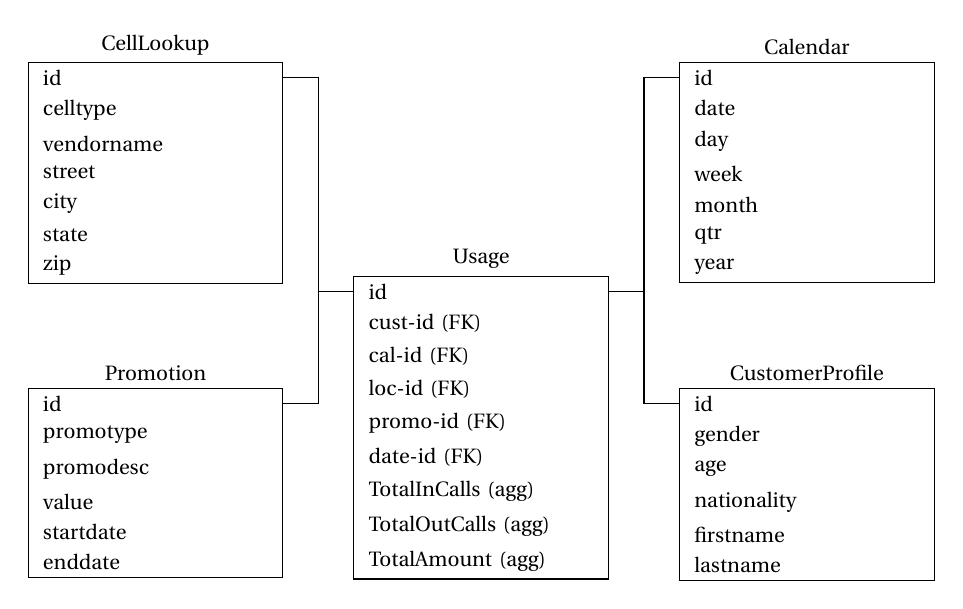
\begin{tikzpicture}[every node/.style={font=\ttfamily}, node distance=1.4in,scale=.75, every node/.style={scale=0.75}]
%https://tex.stackexchange.com/questions/133754/creating-crows-foot-style-e-r-diagrams-rather-than-chen-style-ones
\matrix  [entity=Usage, entity anchor=Usage-id]  {
	\properties{
		id,
		cust-id (FK),
		cal-id (FK), 
		loc-id (FK),
		promo-id (FK),
		date-id (FK),
		TotalInCalls (agg),
		TotalOutCalls (agg),
		TotalAmount (agg)
	}
};


\matrix  [entity=CellLookup, above left=of Usage-id, entity anchor=CellLookup-id]  {
	\properties{
		id,
		celltype,
		vendorname,
		street,
		city,
		state,
		zip
	}
};
\matrix  [entity=Promotion, below left=of Usage-id,yshift=10ex, entity anchor=Promotion-id]  {
	\properties{
		id,
		promotype,
		promodesc,
		value,
		startdate,
		enddate
	}
};

\matrix [entity=CustomerProfile, below right=of Usage-id,yshift=10ex, entity anchor=CustomerProfile-id]  {
	\properties{
		id, 
		gender, 
		age, 
		nationality,
		firstname,
		lastname
	}
};


\matrix  [entity=Calendar, above right=of Usage-id, entity anchor=Calendar-id]  {
	\properties{
		id,
		date,
		day,
		week,
		month,
		qtr,
		year
	}
};

\draw [one to one] (Usage-id)  to (CustomerProfile-id);
\draw [one to one] (Usage-id)  to (Calendar-id);
\draw [one to one] (Usage-id)  to (CellLookup-id);
\draw [one to one] (Usage-id)  to (Promotion-id);

\end{tikzpicture}
}
%%%%%%%%%%%%%%%%%%%%%%%%%%%%%%%%%%%%%%%%%%%%%%%%%%%%%%%%%%%%%%%%%%%%%%%%%%%
%%% Local Variables:
%%% mode: latex
%%% TeX-master: "../../main.tex"
% !TeX root = ../../main.tex
%%% TeX-engine: xetex
%%% End:

\end{frame}

%%%%%%%%%%%%%%%%%%%%%%%%%%%%%%%%%%%%%%%%%%%%%%%%%%%%%%
\midTitle{Data Model: Elements of Data Model}
\begin{frame}
	\frametitle{Elements of Data Model}
		Dimensional model life cycle:
	    \begin{itemize}[<+->]
			\item Gathering Requirements (Source Driven, Business/User Driven).
			\item Identify granularity of the facts
			\item Identify the dimensions
			\item Identify the facts
	    \end{itemize}	
\end{frame}
%%%%%%%%%%%%%%%%%%%%%%%%%%%%%%%%%%%%%%%%%%%%%%%%%%%%%%

\begin{frame}
\frametitle{Dimensions Types}
	\begin{enumerate}[<+->]
		\item Conformed Dimension.
		\item Degenerate Dimension.
		\item Junk Dimension (Garbage Dimension).
		\item Role-Playing Dimension.
		\item Outrigger Dimension.
		\item Snowflake Dimension.
		\item Shrunken Rollup Dimension.
		\item Swappable Dimension.
		\item Slowly changing Dimension.
		\item Fast Changing Dimension (Mini Dimension).
		\item Heterogenous Dimensions
		\item Multi-valued dimensions
	\end{enumerate}
\end{frame}





%%%%%%%%%%%%%%%%%%%%%%%%%%%%%%%%%%%%%%%%%%%%%%%%%%%%%%%%%%%%%%%%%%%%%%%%%%%%
%%% Local Variables:
%%% mode: latex
%%% TeX-master: "../main"
% !TeX root = ../main.tex
%%% TeX-engine: xetex
%%% End:
%-------------------------------------------------------%
%%%%%%%%%%%%%%%%%%%%%%%%%%%%%%%%%%%%%%%%%%%%%%%%%%%%%%%
%\VideoClassification[column=1, colour=blue]
%%%%%%%%%%%%%%%%%%%%%%%%%%%%%%%%%%%%%%%%%%%%%%%%%%%%%%%
%\midTitle{Dimensions Types: Conformed Dimension}
%\begin{frame}
%    \frametitle{Conformed Dimensions}
%    %https://www.guru99.com/dimensional-model-data-warehouse.html
%    %The dimension can also contain one or more hierarchical relationships
%    \begin{description}[<+->]
%        \item[Conformed Dimensions]    the dimension which is \underline{\textit{identical}} and has the \underline{\textit{same meaning}} across many fact tables which it relates and used in different areas of the warehouse.
%        \begin{example}
%            \begin{itemize}[<+->]
%                \item \underline{\textbf{(Date as a Key)}}: if we have a date column across many facts, we could use the date as key in all tables. So, it should be a unified format.
%                \item \underline{\textbf{(Product-Id as a Key)}}: if we have a product name which could vary between systems
%                \forexample (upper/lower) We can create a dimension table for the product details and use product id unified across fact tables.
%            \end{itemize}
%        \end{example}
%    \end{description}
%\end{frame}
%%%%%%%%%%%%%%%%%%%%%%%%%%%%%%%%%%%%%%%%%%%%%%%%%%%%%%%
%\VideoClassification[column=1, colour=blue]
%%%%%%%%%%%%%%%%%%%%%%%%%%%%%%%%%%%%%%%%%%%%%%%%%%%%%%%
%\midTitle{Dimensions Types: Degenerate Dimension}
%\begin{frame}
%	\frametitle{Degenerate Dimensions}
%	%https://www.guru99.com/dimensional-model-data-warehouse.html
%	\begin{itemize}[<+->]
%		\item Degenerate Dimensions
%		\begin{itemize}[<+->]
%			\item Dimension Key without corresponding dimension table.% (Not a fact and not an attribute)
%			\item Stored in fact table.
%			%This kind of dimension does not have its dimension as it is derived from the fact table.
%			\item It used to provide a grouping for business cases.
%		\end{itemize}
%	\end{itemize}
%\end{frame}
%%%%%%%%%%%%%%%%%%%%%%%%%%%%%%%%%%%%%%%%%%%%%%%%%%%%%%%
%%\VideoClassification[column=1, colour=blue]
%%%%%%%%%%%%%%%%%%%%%%%%%%%%%%%%%%%%%%%%%%%%%%%%%%%%%%%
%\begin{frame}
%	\frametitle{Degenerate Dimension}
%	%https://www.guru99.com/dimensional-model-data-warehouse.html
%	\begin{itemize}
%		\item Degenerate Dimensions
%		\begin{itemize}
%			\item Dimension Key without corresponding dimension table.% (Not a fact and not an attribute)
%			\item Stored in fact table.
%			\item It used to provide a grouping for business cases.
%			%This kind of dimension does not have its dimension as it is derived from the fact table.
%		\end{itemize}
%	\end{itemize}
%	\centering
%	\begin{tikzpicture}[every node/.style={font=\ttfamily}, node distance=1.4in,scale=.6, every node/.style={scale=0.6}]
    \matrix  [entity=OrderDetial, entity anchor=OrdersDetial-OrderID]  {
    \properties{
    OrderID,
    OrderDate (FK),
    ProductID (FK),
    Quantity,
    Amount
    }
    };
\end{tikzpicture}

%	
%	\begin{table}[t]
%		\centering
%		\sffamily
%		\begin{tabular}{|a | l | l | l | l|}
%			\hline
%			OrderID  & OrderDate & ProductID & Quantity & Amount\\
%			\hline
%			\hline
%			%\rowcolor{LightCyan}
%			123 & 123456789 & 111 & 2 & 120.45\\
%			123 & 123456789 & 222 & 5 & 10.45\\
%			%\rowcolor{myorange}
%			\hline
%			\hline
%			431 & 98765122 & 333 & 1 & 15.45\\
%			431 & 98765122 & 555 & 6 & 4.45\\
%			\hline
%		\end{tabular}
%	\end{table}
%\end{frame}
%
%%%%%%%%%%%%%%%%%%%%%%%%%%%%%%%%%%%%%%%%%%%%%%%%%%%%%%%
%\VideoClassification[column=1, colour=blue]
%%%%%%%%%%%%%%%%%%%%%%%%%%%%%%%%%%%%%%%%%%%%%%%%%%%%%%%
%\midTitle{Dimensions Types: Junk Dimension (Garbage Dimension)}
%\begin{frame}
%    \frametitle{Junk Dimension}
%    \begin{itemize}[<+->]
%        %junk assume we have multi flags we will collect them as one id
%        \item It used to reduce the number of dimensions (low-cardinality columns) in the dimensional model and reduce the number of columns in the fact table. It is a collection of random transnational codes, flags, or text attributes.
%        \item It optimizes space as fact tables should not include low-cardinality or text fields. It mainly includes measures, foreign keys, and degenerate dimension keys.
%    \end{itemize}
%\end{frame}
%%%%%%%%%%%%%%%%%%%%%%%%%%%%%%%%%%%%%%%%%%%%%%%%%%%%%%%
%\begin{frame}
%    \frametitle{Junk Dimension}
%    %\resizebox{\columnwidth}{!}{%
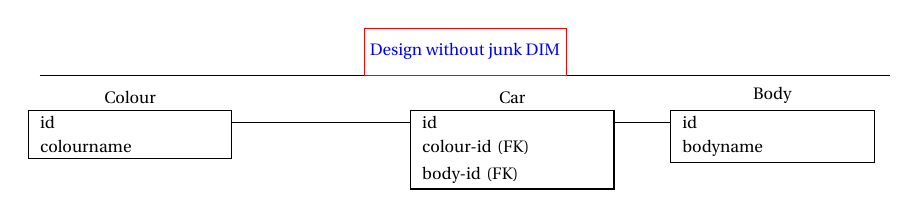
\begin{tikzpicture}[every node/.style={font=\ttfamily}, node distance=1.4in,scale=.6, every node/.style={scale=0.6}]
\matrix  [entity=Car, entity anchor=Car-id]  {
	\properties{
		id,
		colour-id (FK),
		body-id (FK)
	}
};


\matrix  [entity=Colour, left=of Car-id, entity anchor=Colour-id]  {
	\properties{
		id,
		colourname
	}
};
\matrix  [entity=Body, right=of Car-id,xshift=-15ex,entity anchor=Body-id]  {
	\properties{
		id,
		bodyname
	}
};
\draw (-10,1) -- (8,1) node[blue,draw=red, ultra thin, minimum size=1cm] [above,pos=0.5] {Design without junk DIM};
\draw [one to one] (Car-id)  to (Colour-id);
\draw [one to one] (Car-id)  to (Body-id);
\end{tikzpicture}
%}

%\resizebox{\columnwidth}{!}{%
	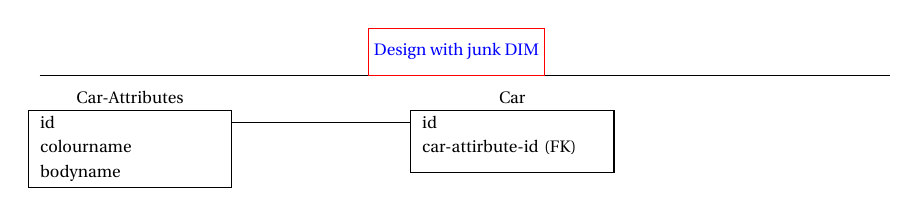
\begin{tikzpicture}[every node/.style={font=\ttfamily}, node distance=1.4in,scale=.6, every node/.style={scale=0.6}]
	
	\matrix  [entity=Car, entity anchor=Car-id]  {
		\properties{
			id,
			car-attirbute-id (FK),
		}
	};	

	\matrix  [entity=Car-Attributes, left=of Car-id, entity anchor=Car-Attributes-id]  {
		\properties{
			id,
			colourname,
			bodyname
		}
	};
	\draw (-10,1) -- (8,1) node[blue,draw=red, ultra thin, minimum size=1cm] [above,pos=0.49] {Design with junk DIM};
	\draw [one to one] (Car-id)  to (Car-Attributes-id);
	\end{tikzpicture}
%}
%%%%%%%%%%%%%%%%%%%%%%%%%%%%%%%%%%%%%%%%%%%%%%%%%%%%%%%%%%%%%%%%%%%%%%%%%%%
%%% Local Variables:
%%% mode: latex
%%% TeX-master: "../../main.tex"
% !TeX root = ../../main.tex
%%% TeX-engine: xetex
%%% End:

%\end{frame}
%%%%%%%%%%%%%%%%%%%%%%%%%%%%%%%%%%%%%%%%%%%%%%%%%%%%%%%
%\begin{frame}
%	\frametitle{Junk Dimension}
%
%	\begin{block}{Junk Dimension Table Size}
%		\begin{itemize}
%			\item We must split the Junk dimension into more dimensions in case the size grows by the time.
%			\item It is easy to calculate the expected number of rows as it is the total number of combinations between the low-cardinality attributes; \forexample 3 columns each have 3 values total = 3 * 3 = 9.
%		\end{itemize}
%	\end{block}
%	
%\end{frame}
%%%%%%%%%%%%%%%%%%%%%%%%%%%%%%%%%%%%%%%%%%%%%%%%%%%%%%%
%\VideoClassification[column=1, colour=blue]
%%%%%%%%%%%%%%%%%%%%%%%%%%%%%%%%%%%%%%%%%%%%%%%%%%%%%%%
%\midTitle{Dimensions Types: Role-Playing Dimension}
%\begin{frame}
%    \frametitle{Role-Playing Dimension}
%    \begin{description}
%        \item [Role-Playing Dimensions (Re-usable Dimension)] A single physical dimension helps to reference multiple times in a fact table as each reference linking to a logically distinct role for the dimension.
%    \end{description}
%    \centering
%    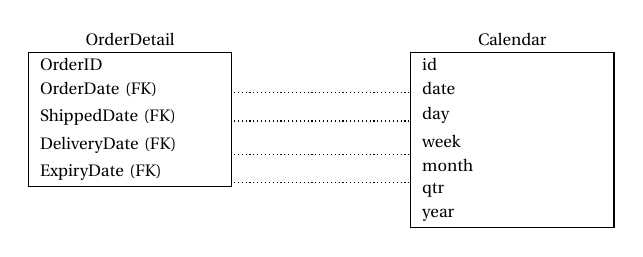
\begin{tikzpicture}[every node/.style={font=\ttfamily}, node distance=1.4in,scale=.6, every node/.style={scale=0.6}]

    \matrix  [entity=OrderDetail, entity anchor=OrderDetail-OrderID]  {
        \properties{
        OrderID,
        OrderDate (FK),
        ShippedDate (FK),
        DeliveryDate (FK),
        ExpiryDate (FK)
        }
    };
    \matrix  [entity=Calendar, right=of OrderDetail-OrderID, entity anchor=Calendar-id] {
        \properties{
        id,
        date,
        day,
        week,
        month,
        qtr,
        year
        }
    };
    %\draw [one to one] (OrderDetail-OrderID)  to (Calendar-id);
    \draw[densely dotted] (2.2,-1.9)  -- (5.9,-1.9);
    \draw[densely dotted] (2.2,-1.2)  -- (5.9,-1.2);
    \draw[densely dotted] (2.2,-.6 )  -- (5.9,-.6);
    \draw[densely dotted] (2.2,-2.5)  -- (5.9,-2.5);
\end{tikzpicture}
%%%%%%%%%%%%%%%%%%%%%%%%%%%%%%%%%%%%%%%%%%%%%%%%%%%%%%%%%%%%%%%%%%%%%%%%%%%
%%% Local Variables:
%%% mode: latex
%%% TeX-master: "../../main.tex"
% !TeX root = ../../main.tex
%%% TeX-engine: xetex
%%% End:

%\end{frame}
%%%%%%%%%%%%%%%%%%%%%%%%%%%%%%%%%%%%%%%%%%%%%%%%%%%%%%%
%\begin{frame}
%    \frametitle{Conformed vs Role-Playing Dimension}
%    \begin{block}{Conformed vs Role-Playing}
%        \begin{itemize}
%            \item \textbf{Conformed} is the same dimension used in different facts and has \textit{\underline{the same meaning}} \forexample CustomerID.
%            \item \textbf{Role-Playing} is the same dimension which used multiple times within the same fact but \textit{\underline{with different meanings}} \forexample Date.
%        \end{itemize}
%    \end{block}
%\end{frame}
%
%%%%%%%%%%%%%%%%%%%%%%%%%%%%%%%%%%%%%%%%%%%%%%%%%%%%%%%
%\VideoClassification[column=1, colour=blue]
%%%%%%%%%%%%%%%%%%%%%%%%%%%%%%%%%%%%%%%%%%%%%%%%%%%%%%%
%\midTitle{Dimensions Types: Outrigger Dimensions}
%\begin{frame}
%    \frametitle{Outrigger Dimensions}
%    \begin{itemize}[<+->]
%        \item A dimension which has a reference to another dimension table. The secondary dimension called outrigger dimension.
%        \item \blue{\textit{\faBullhorn This dimension design should be used carefully without limited cases}}.
%    \end{itemize}
%\end{frame}
%%%%%%%%%%%%%%%%%%%%%%%%%%%%%%%%%%%%%%%%%%%%%%%%%%%%%%%
%\begin{frame}
%    \frametitle{Outrigger Dimensions}
%    \centering
%    \resizebox{.9\columnwidth}{!}{%
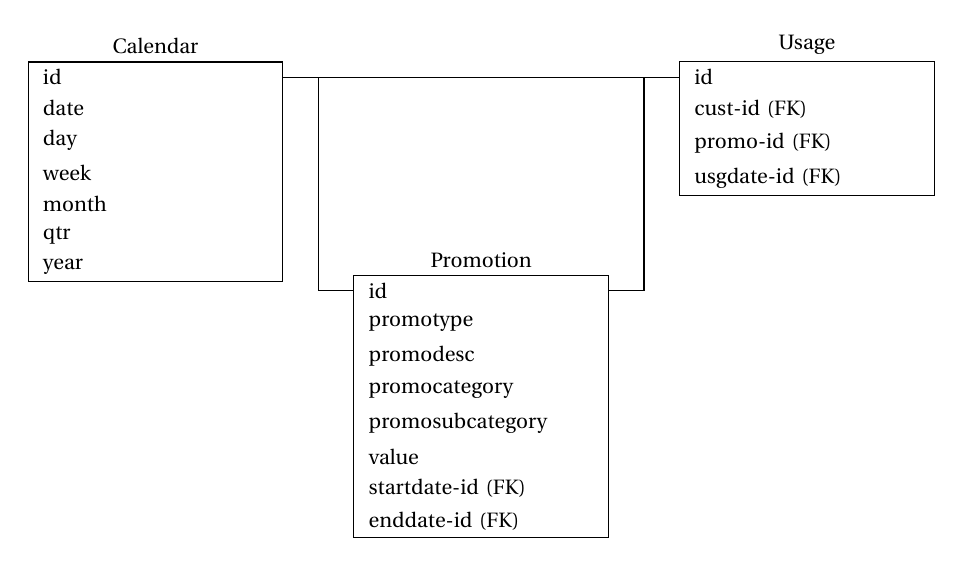
\begin{tikzpicture}[every node/.style={font=\ttfamily}, node distance=1.4in,scale=.75, every node/.style={scale=0.75}]

    \matrix  [entity=Usage, entity anchor=Usage-id]  {
        \properties{
        id,
        cust-id (FK),
        promo-id (FK),
        usgdate-id (FK)
        }
    };

    \matrix  [entity=Promotion, below left=of Usage-id, entity anchor=Promotion-id]  {
        \properties{
        id,
        promotype,
        promodesc,
        promocategory,
        promosubcategory,
        value,
        startdate-id (FK),
        enddate-id (FK)
        }
    };
    \matrix  [entity=Calendar, above left=of Promotion-id, entity anchor=Calendar-id]  {
        \properties{
        id,
        date,
        day,
        week,
        month,
        qtr,
        year
        }
    };

    \draw [one to one] (Usage-id)  to (Promotion-id);
    \draw [one to one] (Promotion-id)  to (Calendar-id);
    \draw [one to one] (Usage-id)  to (Calendar-id);
\end{tikzpicture}
}

%\end{frame}
%
%%%%%%%%%%%%%%%%%%%%%%%%%%%%%%%%%%%%%%%%%%%%%%%%%%%%%%%
%\VideoClassification[column=1, colour=blue]
%%%%%%%%%%%%%%%%%%%%%%%%%%%%%%%%%%%%%%%%%%%%%%%%%%%%%%%
%\midTitle{Dimensions Types: Snowflake Dimensions}
%\begin{frame}
%    \frametitle{Snowflake Dimensions}
%    \begin{itemize}[<+->]
%        \item Snowflake Dimension is a dimension that has a hierarchy of attributes. This attribute is normalized, and each dimension has a relationship with another hierarchy dimension table.\\
%        \item \red{\textit{\faBug This dimension design not recommended as it has much complexity to the model and query performance. Also, it complicates the ETL process and makes too many dimensions without needs}}.
%    \end{itemize}
%\end{frame}
%%%%%%%%%%%%%%%%%%%%%%%%%%%%%%%%%%%%%%%%%%%%%%%%%%%%%%%
%\begin{frame}
%    \frametitle{Snowflake Dimensions}
%    \begin{itemize}
%        \item Snowflake Dimension is a dimension that has a hierarchy of attributes. This attribute is normalized, and each dimension has a relationship with another hierarchy dimension table.\\
%		\item \red{\textit{\faBug This dimension design not recommended as it has much complexity to the model and query performance. Also, it complicates the ETL process and makes too many dimensions without needs}}.
%    \end{itemize}
%    \centering
%    \resizebox{.9\columnwidth}{!}{%
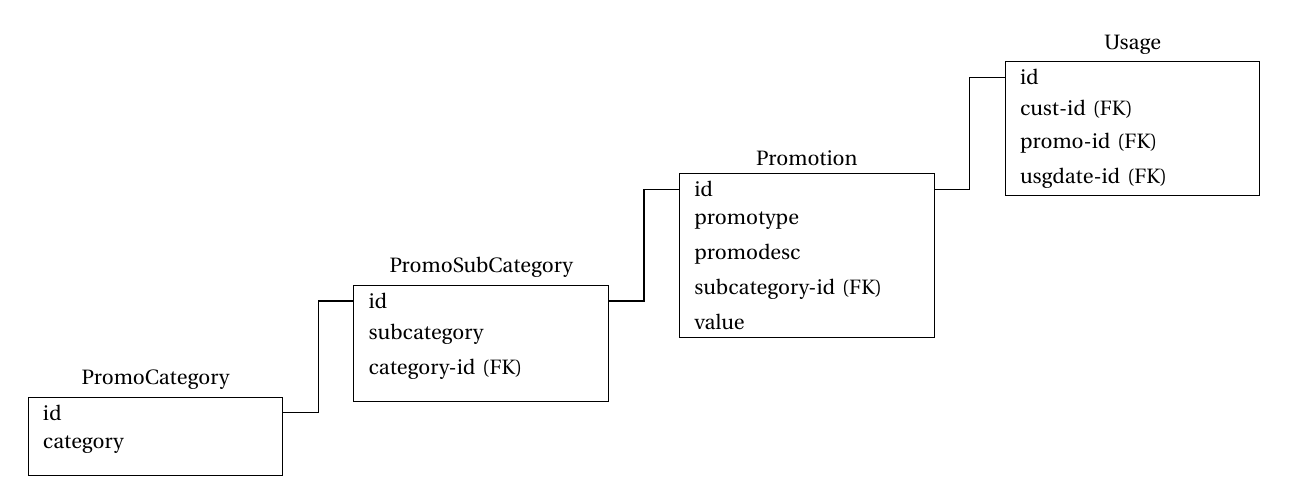
\begin{tikzpicture}[every node/.style={font=\ttfamily}, node distance=1.4in,scale=.75, every node/.style={scale=0.75}]
    \matrix  [entity=Usage, entity anchor=Usage-id]  {
        \properties{
        id,
        cust-id (FK),
        promo-id (FK),
        usgdate-id (FK)
        }
    };
    \matrix  [entity=Promotion, below left=of Usage-id,yshift=10ex, entity anchor=Promotion-id]  {
        \properties{
        id,
        promotype,
        promodesc,
        subcategory-id (FK),
        value
        }
    };
    \matrix  [entity=PromoSubCategory, below left=of Promotion-id,yshift=10ex, entity anchor=PromoSubCategory-id]  {
        \properties{
        id,
        subcategory,
        category-id (FK),
        }
    };
    \matrix  [entity=PromoCategory, below left=of PromoSubCategory-id,yshift=10ex, entity anchor=PromoCategory-id]  {
        \properties{
        id,
        category,
        }
    };


    \draw [one to one] (Usage-id)  to (Promotion-id);
    \draw [one to one] (Promotion-id)  to (PromoSubCategory-id);
    \draw [one to one] (PromoSubCategory-id) to (PromoCategory-id);
\end{tikzpicture}
}

%%%%%%%%%%%%%%%%%%%%%%%%%%%%%%%%%%%%%%%%%%%%%%%%%%%%%%%%%%%%%%%%%%%%%%%%%%%
%%% Local Variables:
%%% mode: latex
%%% TeX-master: "../../main.tex"
% !TeX root = ../../main.tex
%%% TeX-engine: xetex
%%% End:

%\end{frame}
%%%%%%%%%%%%%%%%%%%%%%%%%%%%%%%%%%%%%%%%%%%%%%%%%%%%%%%
%\VideoClassification[column=1, colour=red]
%%%%%%%%%%%%%%%%%%%%%%%%%%%%%%%%%%%%%%%%%%%%%%%%%%%%%%%
%\midTitle{Dimensions Types: Slowly changing Dimensions}
%\begin{frame}
%    \frametitle{Slowly changing Dimensions}
%    %https://www.guru99.com/dimensional-model-data-warehouse.html
%    \begin{itemize}[<+->]
%		\item It the dimension which changes over time. So, for a specific date we have different value.
%		\item It has different types as following
%		    \begin{itemize}[<+->]
%        \item Type 0 (Fixed Dimension): We don't change the current even the source changes. 
%        \item Type 1 (No History): No history is maintained only the latest replace the current.
%        \item Type 2 (History): Series of history of records are maintained.
%        \item Type 3 (Hybrid): Only the last Change and the Current new change is stored
%        \item Type 4 : We split the data into two tables, first the current record and second is the historical (most common usage).
%    \end{itemize}   
%
%
%        %slowly changing dim assume customer was located in dubai then he changed his location
%        % We don't care about the change. just update the latest
%        % we can have two version new, old.
%        % we can have sergeate key.
%        %with start and end data.
%        %start and end is null
%        %join with sergate key
%    \end{itemize}
%\end{frame}
%%%%%%%%%%%%%%%%%%%%%%%%%%%%%%%%%%%%%%%%%%%%%%%%%%%%%%%
%\begin{frame}
%	\frametitle{Slowly changing Dimensions}
%\begin{block}{Note}
%	\textit{There are some other types which is a combination between the above similar than type 3 combined between 1 \& 2. \\ You can check the chapter resources for more information about the other types.}
%\end{block}
%%https://www.kimballgroup.com/2013/02/design-tip-152-slowly-changing-dimension-types-0-4-5-6-7/     
%\end{frame}
%%%%%%%%%%%%%%%%%%%%%%%%%%%%%%%%%%%%%%%%%%%%%%%%%%%%%%%
%\begin{frame}
%	\frametitle{Slowly changing Dimensions}
%	
%	\begin{itemize}
%		\item Type 0.
%	\end{itemize}
%	\begin{table}[t]
%		\centering
%		\sffamily
%		\begin{tabular}{|l | l | a |}
%			\hline
%			CustomerID & Name & City\\
%			\hline
%			\hline			
%			123456789 & Ronaldo  & Madrid\\
%			\hline
%		\end{tabular}
%		\quad
%		\begin{tabular}{|l | l| a|}
%			\hline
%			CustomerID & Name & City\\
%			\hline
%			\hline			
%			123456789 & Ronaldo  & Turin\\
%			\hline
%		\end{tabular}
%		\caption{Source System Old vs New}
%	\end{table}
%	
%	\begin{table}[t]
%		\centering
%		\sffamily
%		\begin{tabular}{|l | l | l |a|}
%			\hline
%			ID & CustomerID & Name & City\\
%			\hline
%			\hline		
%			1 & 123456789 & Ronaldo  & Madrid\\
%			\hline
%		\end{tabular}
%		\caption{Customer Profile Dimension}
%	\end{table}
%		
%\end{frame}
%%%%%%%%%%%%%%%%%%%%%%%%%%%%%%%%%%%%%%%%%%%%%%%%%%%%%%%
%\begin{frame}
%	\frametitle{Slowly changing Dimensions}
%	
%	\begin{itemize}
%		\item Type 1.
%	\end{itemize}
%	\begin{table}[t]
%		\centering
%		\sffamily
%		\begin{tabular}{|l | l | a |}
%			\hline
%			CustomerID & Name & City\\
%			\hline
%			\hline			
%			123456789 & Ronaldo  & Madrid\\
%			\hline
%		\end{tabular}
%		\quad
%		\begin{tabular}{|l | l| a|}
%			\hline
%			CustomerID & Name & City\\
%			\hline
%			\hline			
%			123456789 & Ronaldo  & Turin\\
%			\hline
%		\end{tabular}
%		\caption{Source System Old vs New}
%	\end{table}
%	
%	\begin{table}[t]
%		\centering
%		\sffamily
%		\begin{tabular}{|l | l | l |a|}
%			\hline
%			ID & CustomerID & Name & City\\
%			\hline
%			\hline		
%			1 & 123456789 & Ronaldo  & Turin\\
%			\hline
%		\end{tabular}
%		\caption{Customer Profile Dimension}
%	\end{table}	
%\end{frame}
%%%%%%%%%%%%%%%%%%%%%%%%%%%%%%%%%%%%%%%%%%%%%%%%%%%%%%%
%\begin{frame}
%	\frametitle{Slowly changing Dimensions}
%	\begin{itemize}
%		\item Type 2.
%	\end{itemize}
%	\begin{table}[t]
%		\centering
%		\sffamily
%		\begin{tabular}{|l | l | a |l|}
%			\hline
%			CustomerID & Name & City & UpdatedDt \\
%			\hline
%			\hline			
%			123456789 & Ronaldo  & Madrid & 2018-12-12\\
%			\hline
%			\hline			
%			123456789 & Ronaldo  & Turin & 2019-06-12\\
%			\hline
%			\hline			
%			123456789 & Ronaldo  & London & 2019-08-12\\
%			\hline
%			\hline						
%			123456789 & Ronaldo  & Porto & 2019-12-12\\		
%			\hline
%		\end{tabular}	
%		\caption{Source System Old vs New}
%	\end{table}%
%	\vspace{-.8cm}
%
%	\begin{table}[t]
%		\centering
%		\sffamily
%		  \begin{adjustbox}{max width=\textwidth}			
%		\begin{tabular}{|l | l | l | a | l | l |a|}
%			\hline
%			ID & CustomerID & Name & City & effectiveDt & TerminationDt & isCurrent\\
%			\hline
%			\hline		
%			1 & 123456789 & Ronaldo  & Madrid & 2018-12-12 & 2019-06-12 & false\\
%			2 & 123456789 & Ronaldo  & Turin & 2019-06-12 & 2019-08-12 & false\\
%			3 & 123456789 & Ronaldo  & London & 2019-08-12 & 2019-12-12 & false\\
%			4 & 123456789 & Ronaldo  & Porto  & 2019-12-12 & null & true\\
%			\hline
%		\end{tabular}
%		\end{adjustbox}
%
%		\caption{Customer Profile Dimension {\scriptsize We can replace null with a finite date (9999-12-31) but it needs to be consistent}}
%	\end{table}
%	
%\end{frame}
%%%%%%%%%%%%%%%%%%%%%%%%%%%%%%%%%%%%%%%%%%%%%%%%%%%%%%%
%\begin{frame}
%	\frametitle{Slowly changing Dimensions}
%	\begin{itemize}
%		\item Type 3.
%	\end{itemize}
%	\begin{table}[t]
%		\centering
%		\sffamily
%		\begin{tabular}{|l | l | a |l|}
%			\hline
%			CustomerID & Name & City & UpdatedDt \\
%			\hline
%			\hline			
%			123456789 & Ronaldo  & Madrid & 2018-12-12\\
%			\hline
%			\hline			
%			123456789 & Ronaldo  & Turin & 2019-06-12\\
%			\hline
%			\hline			
%			123456789 & Ronaldo  & London & 2019-08-12\\
%			\hline
%			\hline						
%			123456789 & Ronaldo  & Porto & 2019-12-12\\		
%			\hline
%		\end{tabular}	
%		\caption{Source System Old vs New}
%		
%	\end{table}
%	
%	\begin{table}[t]
%		\centering
%		\sffamily
%		\begin{tabular}{|l | l | l | a | l | l |}
%			\hline
%			ID & CustomerID & Name & City & UpdatedDate  & previousCity\\
%			\hline
%			\hline		
%			1 & 123456789 & Ronaldo  & Porto  & 2019-12-12 & London\\
%			\hline
%		\end{tabular}
%		\caption{Customer Profile Dimension}
%	\end{table}
%\end{frame}
%
%%%%%%%%%%%%%%%%%%%%%%%%%%%%%%%%%%%%%%%%%%%%%%%%%%%%%%%
%\begin{frame}
%	\frametitle{Slowly changing Dimensions}
%	\begin{itemize}
%		\item Type 4 (Split current and Historical).
%	\end{itemize}
%
%	\begin{table}[t]
%	\centering
%	\sffamily
%	\begin{tabular}{|l | l | l | a | l | l |a|}
%		\hline
%		ID & CustomerID & Name & City & effectiveDt & TerminationDt\\
%		\hline
%		\hline		
%		1 & 123456789 & Ronaldo  & Madrid & 2018-12-12 & 2019-06-12\\
%		2 & 123456789 & Ronaldo  & Turin & 2019-06-12 & 2019-08-12\\
%		3 & 123456789 & Ronaldo  & London & 2019-08-12 & 2019-12-12\\
%		4 & 123456789 & Ronaldo  & Porto  & 2019-12-12 & null\\
%		\hline
%	\end{tabular}
%	\caption{Customer Profile Dimension Hist}
%\end{table}
%
%	
%	\begin{table}[t]
%		\centering
%		\sffamily
%		\begin{tabular}{|l | l | l | a | l |}
%			\hline
%			ID & CustomerID & Name & City & UpdatedDate\\
%			\hline
%			\hline		
%			1 & 123456789 & Ronaldo  & Porto  & 2019-12-12\\
%			\hline
%		\end{tabular}
%		\caption{Customer Profile Dimension}
%	\end{table}
%
%\end{frame}
%
%%%%%%%%%%%%%%%%%%%%%%%%%%%%%%%%%%%%%%%%%%%%%%%%%%%%%%%
%\begin{frame}[fragile]
%	\frametitle{Slowly changing Dimensions}
%	\begin{itemize}
%		\item How does the Facts join SCD? We have two scenarios as following:
%		\begin{itemize}
%			\item Getting the current customer information (Join with the latest).
%			\item Getting the historical customer information (Join with the historical table based on \textbf{\textit{cust id \& date}}).
%		\end{itemize}
%	\end{itemize}
%
%	\begin{table}[t]
%		\centering
%		\sffamily
%		\begin{tabular}{|l | a | l | l |}
%			\hline
%			ID & CustomerID & TotalCalls & CallDate \\
%			\hline
%			\hline		
%			1 & 123456789 & 30 & 2018-12-12 \\
%			2 & 123456789 & 30 & 2019-12-12 \\
%			\hline
%		\end{tabular}
%		\caption{Customer Usage}
%	\end{table}
%
%	
%\end{frame}
%%%%%%%%%%%%%%%%%%%%%%%%%%%%%%%%%%%%%%%%%%%%%%%%%%%%%%%
%
%%%%%%%%%%%%%%%%%%%%%%%%%%%%%%%%%%%%%%%%%%%%%%%%%%%%%%%%
%\begin{frame}[fragile]
%	\frametitle{Slowly changing Dimensions}
%	
%	\lstinputlisting[language=sql,caption={Example to show how to use SCD}]{./Ch01-Introduction-data-management/Code/SCD_Examply.sql}
%	
%\end{frame}
%
%%%%%%%%%%%%%%%%%%%%%%%%%%%%%%%%%%%%%%%%%%%%%%%%%%%%%%
%\VideoClassification[column=1, colour=blue]
%%%%%%%%%%%%%%%%%%%%%%%%%%%%%%%%%%%%%%%%%%%%%%%%%%%%%%
%\midTitle{Dimensions Types: Fast (Rapidly) Changing Dimension (Mini Dimension) }
%\begin{frame}
%	\frametitle{Fast Changing Dimension (Mini Dimension)}
%	\begin{itemize}[<+->]
%		\item When we have a dimension with one or more of its attributes changing very fast. 
%		
%		\item \blue{\textit{\faBullhorn \space It causes a performance issue if we tried to handle this case similar SCD Type 2 because of the rapidly changing  in this dimension and the table will includes a lot of rows for this dimension}}.
%
%		\item We solve this case by separation the attributes into one or more dimensions. This technique also called \textit{\textbf{mini-dimensions}}.		
%	
%	\end{itemize}
%\end{frame}
%%%%%%%%%%%%%%%%%%%%%%%%%%%%%%%%%%%%%%%%%%%%%%%%%%%%%%
%\begin{frame}
%	\frametitle{Fast Changing Dimension (Mini Dimension)}
%	\begin{itemize}[<+->]
%		\item How to implement FCD (Mini Dimension)? \underline{{\footnotesize \textit{Hint: Search for the mini-dimension  relation table.}}}
%	\end{itemize}
%
%\begin{table}
%	\begin{adjustbox}{max width=.95\textwidth}			
%		\begin{tabular}{| l | l | l | l | a | a | l|}
%			\hline
%			Patient\_id & Name & Gender & BirthDate & Weight & B\_Presaure & UpdateDt\\
%			\hline
%			\hline		
%			123 & Anna   & F & 1968-01-12 & 50 & 110.0 &2019-01-01\\
%			123 & Anna   & F & 1968-01-12 & 55 & 130.0 &2019-01-07\\
%			123 & Anna   & F & 1968-01-12 & 59 & 115.0 &2019-01-14\\
%			123 & Anna   & F & 1968-01-12 & 65 & 120.0 &2019-01-21\\
%			\hline
%		\end{tabular}
%	\end{adjustbox}
%	\caption{Patient Profile Dimension}
%\end{table}
%
%\begin{table}
%	\resizebox{.97\columnwidth}{!}{%
%		
%		\begin{tabular}{| l | l | l | l |}
%			\hline
%			Patient\_id & Name & Gender & BirthDate \\
%			\hline 
%			\hline		
%			123 & Anna   & F & 1968-01-12 \\
%			\hline
%		\end{tabular}
%
%\quad
%
%		\begin{tabular}{| l | l | l | l |}
%			\hline
%			Patient\_Key & Weight & B\_Presure \\
%			\hline
%			\hline		
%			1 & 50 & 110.0\\
%			2 & 55 & 130.0\\
%			3 & 59 & 115.0\\
%			4 & 65 & 120.0\\
%			\hline
%		\end{tabular}
%	}
%	\caption{Patient Profile Dimension After Removing FCD and Split it into Junk-Dimension table}
%\end{table}
%
%\end{frame}
%
%%%%%%%%%%%%%%%%%%%%%%%%%%%%%%%%%%%%%%%%%%%%%%%%%%%%%%
%\begin{frame}
%	\frametitle{Fast Changing Dimension (Mini Dimension)}
%
%\begin{table}
%	\begin{adjustbox}{max width=.7\textwidth}
%		\begin{tabular}{| l | l | l | l |}
%			\hline
%			Patient\_id & Patient\_Key & Start\_Date & End\_Date\\
%			\hline
%			\hline		
%			123 & 1   & 2019-01-01 & 2019-01-07\\
%			123 & 2   & 2019-01-07 & 2019-01-14\\
%			123 & 3   & 2019-01-14 & 2019-01-21\\
%			123 & 4   & 2019-01-21 & null\\
%			\hline
%		\end{tabular}
%	\end{adjustbox}
%	\caption{Patient Mini Dimension}
%\end{table}
%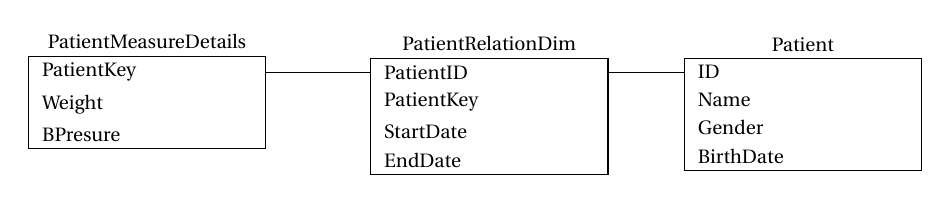
\begin{tikzpicture}[every node/.style={font=\ttfamily}, node distance=1.4in,scale=.7, every node/.style={scale=0.7}]
  
    \matrix  [entity=Patient, entity anchor=Patient-ID]  {
	    \properties{
	    ID,
	    Name,
	    Gender,
	    BirthDate
	    }
    };
    \matrix  [entity=PatientRelationDim, left=of Patient-ID,xshift=9ex,entity anchor=PatientRelationDim-PatientID]  {
		\properties{
			PatientID,
			PatientKey,
			StartDate,
			EndDate
		}
	};
%
	\matrix  [entity=PatientMeasureDetails, left=of PatientRelationDim-PatientID,xshift=6ex, entity anchor=PatientMeasureDetails-PatientKey]  {
		\properties{
			PatientKey,
			Weight,
			BPresure
		}
	};

\draw [one to one] (Patient-ID)  to (PatientRelationDim-PatientID);
\draw [one to one] (PatientRelationDim-PatientID)  to (PatientMeasureDetails-PatientKey);

\end{tikzpicture}

%%%%%%%%%%%%%%%%%%%%%%%%%%%%%%%%%%%%%%%%%%%%%%%%%%%%%%%%%%%%%%%%%%%%%%%%%%%
%%% Local Variables:
%%% mode: latex
%%% TeX-master: "../../main.tex"
% !TeX root = ../../main.tex
%%% TeX-engine: xetex
%%% End:

%\end{frame}
%%%%%%%%%%%%%%%%%%%%%%%%%%%%%%%%%%%%%%%%%%%%%%%%%%%%%%%%
%\VideoClassification[column=1, colour=blue]
%%%%%%%%%%%%%%%%%%%%%%%%%%%%%%%%%%%%%%%%%%%%%%%%%%%%%%%
%\midTitle{Dimensions Types: Shrunken Rollup Dimensions}
%\begin{frame}
%    \frametitle{Shrunken Rollup Dimensions}%منكمش
%    \begin{itemize}[<+->]    	
%		\item Shrunken Rollup dimension is used for developing aggregate (higher level of summary) fact tables. 
%		\item It required that the data model has a lower level of granularity.
%	\end{itemize}
%		\begin{example}
%		    \begin{itemize}[<+->]    	
%			\item We have a daily usage fact table, and we need to have a higher level of monthly usage. So, we use the monthly dimension to get a summary of the daily.
%			\item We have a daily usage fact table aggregated on area-id, and we need to create another summary table aggregated based on city id. So, the new grain level here is the new dimension for the city.
%			\end{itemize}
%		\end{example}
%\end{frame}
%%%%%%%%%%%%%%%%%%%%%%%%%%%%%%%%%%%%%%%%%%%%%%%%%%%%%%%
%\begin{frame}
%	\frametitle{Shrunken Rollup Dimensions Cont.}
%
%	\begin{table}[t]
%		\centering
%		\sffamily
%		\begin{tabular}{|l | a | l |}
%			\hline
%			OrderDate & AreaID & TotalOrders\\
%			\hline
%			\hline
%			123456789 & 123  & 20\\
%			123456789 & 123  & 30\\
%			\hline
%			\hline
%			123456789 & 678  & 10\\
%			123456789 & 678  & 12\\
%			\hline
%		\end{tabular}
%
%	\end{table}
%	
%	\begin{table}[t]
%		\centering
%		\sffamily
%		\begin{tabular}{|a | l | l |}
%			\hline
%			AreaID & AreaName & CityID\\
%			\hline
%			\hline			
%			123 & Al-Matareya  & 1\\
%			678 & Ain shams    & 1\\
%			\hline
%		\end{tabular}
%		\quad
%		\begin{tabular}{|a | l|}
%			\hline
%			CityID & CityName\\
%			\hline
%			\hline			
%			1 & Cairo \\
%			\hline
%		\end{tabular}
%	\end{table}
%
%	\begin{table}[t]
%	\centering
%	\sffamily
%		\begin{tabular}{|l | a | l |}
%			\hline
%			OrderDate & CityID & TotalOrders\\
%			\hline
%			\hline		
%			123456789 & 1  & 72\\
%			\hline
%		\end{tabular}
%	\end{table}
%\end{frame}
%%%%%%%%%%%%%%%%%%%%%%%%%%%%%%%%%%%%%%%%%%%%%%%%%%%%%%
\VideoClassification[column=1, colour=blue]
%%%%%%%%%%%%%%%%%%%%%%%%%%%%%%%%%%%%%%%%%%%%%%%%%%%%%%
\midTitle{Dimensions Types: Multi-valued dimensions (Many-To-Many Dimension)}
\begin{frame}
	\frametitle{Multi-valued dimensions}
	\begin{itemize}[<+->]
		\item When the relationships between the dimension member and the fact are many to many which means the dimension members are lower granularity than the facts. 
		\item Fact table should contains one-to-one relationship with the dimension. So, we introduce the \textbf{\textit{Bridge table}} when we need to related multiple dimensions values with one record.
	\end{itemize}
	
	\begin{example}
		\begin{itemize}[<+->]
			\item Patients can have multiple diagnoses.
			\item Students can have multiple majors.
			\item customers can have multiple account.
			\item Authors can have multiple publications.
		\end{itemize}
	\end{example}		
	
\end{frame}
%%%%%%%%%%%%%%%%%%%%%%%%%%%%%%%%%%%%%%%%%%%%%%%%%%%%%%
\begin{frame}
	\frametitle{Multi-valued dimensions}
	\begin{example}[Sales of Articles]
		\begin{itemize}[<+->]
			\item Assume we need to report the sales of article and we have some articles has more than one author.
			\item According to the report we need to check each author and associate with the articles they have authored. How can we model this case?
		\end{itemize}
	\end{example}
	\begin{tikzpicture}[every node/.style={font=\ttfamily}, node distance=1.4in,scale=.7, every node/.style={scale=0.7}]
  
    \matrix  [entity=Author, entity anchor=Author-ID]  {
	    \properties{
	    ID,
	    Name,
	    Email,
	    Bio
	    }
    };
    \matrix  [entity=AuthorGroupRelation, left=of Author-ID,xshift=9ex,entity anchor=AuthorGroupRelation-ID]  {
		\properties{
			ID,
			AuthorKey,
			WieghtingFactor
		}
	};
%
	\matrix  [entity=AuthorGroup, left=of AuthorGroupRelation-ID,xshift=6ex, entity anchor=AuthorGroup-ID]  {
		\properties{
			ID
		}
	};

	\matrix  [entity=ArticleSales, below right =of AuthorGroup-ID,yshift=7ex,xshift=-6ex, entity anchor=ArticleSales-ID]  {
	\properties{
		ID,
		AuthorGroupID,
		SalesDt,
		Quantity,
		UnitPrice
	}
	};

	\matrix  [entity=Article,  right =of ArticleSales-ID, entity anchor=Article-ID]  {
	\properties{
		ID,
		Title,
		Journal,
		Volume,
		Price
	}
};


\draw [one to many] (Author-ID)  to (AuthorGroupRelation-ID);
\draw [many to one] (AuthorGroupRelation-ID) to (AuthorGroup-ID);
\draw [many to one] (ArticleSales-ID)  to (AuthorGroup-ID);
\draw [many to one] (ArticleSales-ID)  to (Article-ID);
\end{tikzpicture}

%%%%%%%%%%%%%%%%%%%%%%%%%%%%%%%%%%%%%%%%%%%%%%%%%%%%%%%%%%%%%%%%%%%%%%%%%%%
%%% Local Variables:
%%% mode: latex
%%% TeX-master: "../../main.tex"
% !TeX root = ../../main.tex
%%% TeX-engine: xetex
%%% End:

\end{frame}

%multi-valued attributes is to create a relationship between the dimension table and a secondary dimensional table (outrigger table).
%
\textbf{}
%%%%%%%%%%%%%%%%%%%%%%%%%%%%%%%%%%%%%%%%%%%%%%%%%%%%%%
\VideoClassification[column=1, colour=blue]
%%%%%%%%%%%%%%%%%%%%%%%%%%%%%%%%%%%%%%%%%%%%%%%%%%%%%%
\midTitle{Dimensions Types: Heterogeneous Dimensions}
\begin{frame}
\frametitle{Heterogeneous Dimensions}
\begin{itemize}[<+->]
	
	\item This type works when we have a case that a company selling different product to the same base of customer. Every product has it different attributes. 
	\item One famous example of this type assume an insurance company has two types of product like health and car. In this case Car insurance has different attributes than the health insurance.
	\item If we tried to model this two different products this type name Heterogeneous dimensions. 
\end{itemize}
\end{frame}
%%%%%%%%%%%%%%%%%%%%%%%%%%%%%%%%%%%%%%%%%%%%%%%%%%%%%%
\begin{frame}
	\frametitle{Heterogeneous Dimensions}
	\begin{itemize}[<+->]		
		\item There are different scenario to implement this type
		\begin{description}
			\item [Separate Dimensions] Split each one in separate dimensions and facts. It will be less data and business will do this analysis from two separate facts.
			\item [Merge Attributes] We will merge all the attributes in one single table and we will add the common attributes and null for un related attributes. Implementing this scenarios when we have less different of attributes. However, this implementation is not recommended because of the table size, performance, and maintenance.
			\item [Generic Design] In this approach we will create a single fact table and single dimension with the common attributes. The problem of this design we will report or care about the common attributes only.
		\end{description}		
\end{itemize}
\end{frame}
%%%%%%%%%%%%%%%%%%%%%%%%%%%%%%%%%%%%%%%%%%%%%%%%%%%%%%
%-------------------------------------------------------%
%%%%%%%%%%%%%%%%%%%%%%%%%%%%%%%%%%%%%%%%%%%%%%%%%%%%%%
\VideoClassification[column=1, colour=blue]
%%%%%%%%%%%%%%%%%%%%%%%%%%%%%%%%%%%%%%%%%%%%%%%%%%%%%%

\midTitle{Schema Types}
\begin{frame}
\frametitle{Schema Types}
	\begin{itemize}[<+->]
		\item Star schema.
		\item Snowflake schema.
	\end{itemize}
	
\end{frame}
%%%%%%%%%%%%%%%%%%%%%%%%%%%%%%%%%%%%%%%%%%%%%%%%%%%%%%
%%%%%%%%%%%%%%%%%%%%%%%%%%%%%%%%%%%%%%%%%%%%%%%%%%%%%%
\midTitle{Schema Types: Star schema}
\begin{frame}
    \frametitle{Schema Types: Star schema}
			\begin{itemize}
				\item \textbf{Star Schema} the center of the star can have one fact table and a number of associated dimension tables. It is known as star schema as its structure resembles a star. The star schema is the simplest type of Data Warehouse schema. It is also known as Star Join Schema and is optimized for querying large data sets.
			\end{itemize}
%     primary dim & secondary 2 level only 
    %snawflake multi dim nationality for example egypt
    %it will scan the nationality first and it will be fortign key with forign key inner join
\end{frame}
%%%%%%%%%%%%%%%%%%%%%%%%%%%%%%%%%%%%%%%%%%%%%%%%%%%%%%
\begin{frame}
\frametitle{Schema Types: Star schema}
\begin{itemize}
	\item Characteristics of Star Schema:
	\begin{itemize}
		\item Every dimension in a star schema is represented with the only one-dimension table.
		\item The dimension table should contain the set of attributes.
		\item The dimension table is joined to the fact table using a foreign key
		\item The dimension table are not joined to each other
		\item Fact table would contain key and measure
		\item The Star schema is easy to understand and provides optimal disk usage.
		\item The dimension tables are not normalized. For instance, in the above figure, Country\_ID does not have Country lookup table as an OLTP design would have.
		\item The schema is widely supported by BI Tools
	\end{itemize}
\end{itemize}
\end{frame}
%%%%%%%%%%%%%%%%%%%%%%%%%%%%%%%%%%%%%%%%%%%%%%%%%%%%%%
\begin{frame}
\frametitle{Schema Types: Star schema (Example)}


\resizebox{\columnwidth}{!}{%
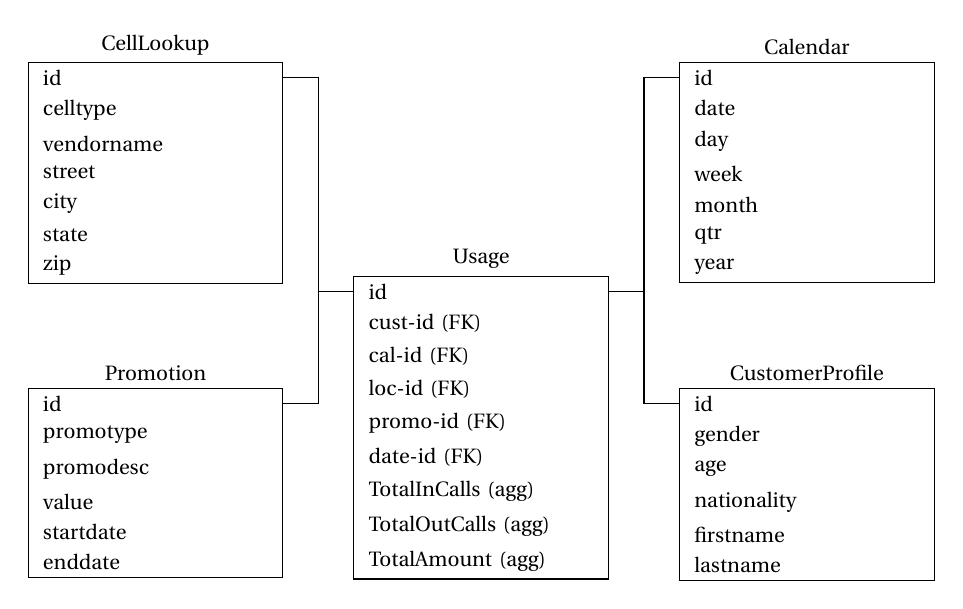
\begin{tikzpicture}[every node/.style={font=\ttfamily}, node distance=1.4in,scale=.75, every node/.style={scale=0.75}]
%https://tex.stackexchange.com/questions/133754/creating-crows-foot-style-e-r-diagrams-rather-than-chen-style-ones
\matrix  [entity=Usage, entity anchor=Usage-id]  {
	\properties{
		id,
		cust-id (FK),
		cal-id (FK), 
		loc-id (FK),
		promo-id (FK),
		date-id (FK),
		TotalInCalls (agg),
		TotalOutCalls (agg),
		TotalAmount (agg)
	}
};


\matrix  [entity=CellLookup, above left=of Usage-id, entity anchor=CellLookup-id]  {
	\properties{
		id,
		celltype,
		vendorname,
		street,
		city,
		state,
		zip
	}
};
\matrix  [entity=Promotion, below left=of Usage-id,yshift=10ex, entity anchor=Promotion-id]  {
	\properties{
		id,
		promotype,
		promodesc,
		value,
		startdate,
		enddate
	}
};

\matrix [entity=CustomerProfile, below right=of Usage-id,yshift=10ex, entity anchor=CustomerProfile-id]  {
	\properties{
		id, 
		gender, 
		age, 
		nationality,
		firstname,
		lastname
	}
};


\matrix  [entity=Calendar, above right=of Usage-id, entity anchor=Calendar-id]  {
	\properties{
		id,
		date,
		day,
		week,
		month,
		qtr,
		year
	}
};

\draw [one to one] (Usage-id)  to (CustomerProfile-id);
\draw [one to one] (Usage-id)  to (Calendar-id);
\draw [one to one] (Usage-id)  to (CellLookup-id);
\draw [one to one] (Usage-id)  to (Promotion-id);

\end{tikzpicture}
}
%%%%%%%%%%%%%%%%%%%%%%%%%%%%%%%%%%%%%%%%%%%%%%%%%%%%%%%%%%%%%%%%%%%%%%%%%%%
%%% Local Variables:
%%% mode: latex
%%% TeX-master: "../../main.tex"
% !TeX root = ../../main.tex
%%% TeX-engine: xetex
%%% End:

\end{frame}
%%%%%%%%%%%%%%%%%%%%%%%%%%%%%%%%%%%%%%%%%%%%%%%%%%%%%%%
\midTitle{Schema Types: Snowflake  schema}
\begin{frame}
\frametitle{Schema Types: Snowflake  schema}
	\begin{itemize}
		\item \textbf{Snowflake Schema} is an extension of a Star Schema, and it adds additional dimensions. It is called snowflake because its diagram resembles a Snowflake. The dimension tables are normalized which splits data into additional tables. In the following example, Country is further normalized into an individual table.
	\end{itemize}
\end{frame}

%%%%%%%%%%%%%%%%%%%%%%%%%%%%%%%%%%%%%%%%%%%%%%%%%%%%%%%
\begin{frame}
\frametitle{Schema Types: Snowflake  schema}
\begin{itemize}
	\item Characteristics of Snowflake Schema:
	\begin{itemize}
		\item The main benefit of the snowflake schema it uses smaller disk space.
		\item Easier to implement a dimension is added to the Schema
		\item Due to multiple tables query performance is reduced
		\item The primary challenge that you will face while using the snowflake Schema is that you need to perform more maintenance efforts because of the more lookup tables.
	\end{itemize}
\end{itemize}
\end{frame}

%%%%%%%%%%%%%%%%%%%%%%%%%%%%%%%%%%%%%%%%%%%%%%%%%%%%%%
\begin{frame}
	\frametitle{Schema Types: Star schema (Example)}
	
	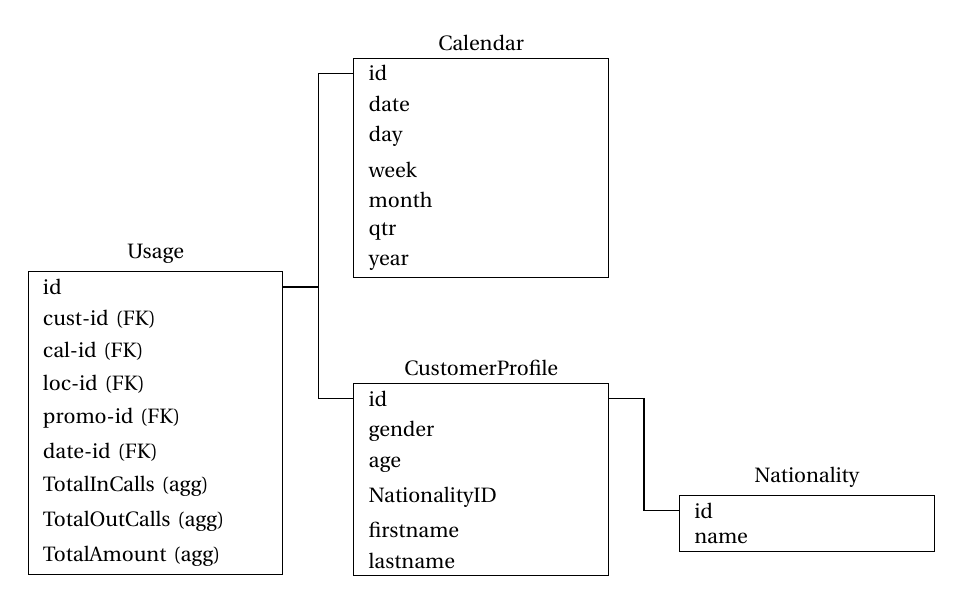
\begin{tikzpicture}[every node/.style={font=\ttfamily}, node distance=1.4in,scale=.75, every node/.style={scale=0.75}]
%https://tex.stackexchange.com/questions/133754/creating-crows-foot-style-e-r-diagrams-rather-than-chen-style-ones
\matrix  [entity=Usage, entity anchor=Usage-id]  {
	\properties{
		id,
		cust-id (FK),
		cal-id (FK), 
		loc-id (FK),
		promo-id (FK),
		date-id (FK),
		TotalInCalls (agg),
		TotalOutCalls (agg),
		TotalAmount (agg)
	}
};


\matrix [entity=CustomerProfile, below right=of Usage-id,yshift=10ex, entity anchor=CustomerProfile-id]  {
	\properties{
		id, 
		gender, 
		age, 
		NationalityID,
		firstname,
		lastname
	}
};

\matrix [entity=Nationality, below right=of CustomerProfile-id,yshift=10ex, entity anchor=Nationality-id]  {
	\properties{
		id, 
		name
	}
};


\matrix  [entity=Calendar, above right=of Usage-id, entity anchor=Calendar-id]  {
	\properties{
		id,
		date,
		day,
		week,
		month,
		qtr,
		year
	}
};

\draw [one to one] (Usage-id)  to (CustomerProfile-id);
\draw [one to one] (Usage-id)  to (Calendar-id);
\draw [one to one] (CustomerProfile-id)  to (Nationality-id);

\end{tikzpicture}
%%%%%%%%%%%%%%%%%%%%%%%%%%%%%%%%%%%%%%%%%%%%%%%%%%%%%%%%%%%%%%%%%%%%%%%%%%%
%%% Local Variables:
%%% mode: latex
%%% TeX-master: "../../main.tex"
% !TeX root = ../../main.tex
%%% TeX-engine: xetex
%%% End:

\end{frame}

%%%%%%%%%%%%%%%%%%%%%%%%%%%%%%%%%%%%%%%%%%%%%%%%%%%%%%%
\begin{frame}
\frametitle{Star Vs Snowflake Schema}

	\begin{tabular}{| l | l |}
		\hline
		Star & Snowflake\\
		\hline
		 \makecell{Hierarchies of the dimensions\\are stored in the dimensional table} &  \makecell{Hierarchies are divided\\ into separate tables}\\
		 		\hline
		\makecell{Fact table surrounded\\ by dimension tables} & 
		\makecell{One fact table surrounded by\\multi-level of dimension tables} \\
				\hline
		 \makecell{Single join creates the\\relation between fact \& dimensions}
		 & \makecell{Requires many joins\\ to fetch the data}\\
 		\hline
		Simple DB Design & Very Complex DB Design\\
		\hline
		De-normalized Data structure & Normalized Data Structure\\
		\hline
		High level of Data redundancy & Very low-level data redundancy\\
		\hline
		Cube processing is faster & Cube processing is slow\\% (complex join)
		\hline
	\end{tabular}


\end{frame}





%%%%%%%%%%%%%%%%%%%%%%%%%%%%%%%%%%%%%%%%%%%%%%%%%%%%%%%%%%%%%%%%%%%%%%%%%%%%
%%% Local Variables:
%%% mode: latex
%%% TeX-master: "../main"
% !TeX root = ../main.tex
%%% TeX-engine: xetex
%%% End:
%-------------------------------------------------------%
\input{./Ch01-Introduction-data-management/12_Data_Model_Selected_Topics.tex}
%-------------------------------------------------------%
%%%%%%%%%%%%%%%%%%%%%%%%%%%%%%%%%%%%%%%%%%%%%%%%%%%%%%
\subsubsection{ETL Process}

\begin{frame}
    \frametitle{What is ETL?}

    \begin{itemize}[<+->]
        \item The ETL (Extraction, Transformation, Loading) is main core function for any data engineering (DWH) team.
        \item This team takes the delivered output from the previous stage (data modeling) and start to implement the mapping.
        \item The implementation of the ETL preferred to be unified across the team members and the organization unless there is a special case of license of capacity.

    \end{itemize}


\end{frame}
%%%%%%%%%%%%%%%%%%%%%%%%%%%%%%%%%%%%%%%%%%%%%%%%%%%%%%

\begin{frame}
    \frametitle{ETL Characteristics}
    %%https://www.timmitchell.net/etl-best-practices/
    \begin{itemize}[<+->]
        \item Successful ETL design have the following characteristics:
        \begin{itemize}[<+->]
            \item [\faCheckSquareO] Maintainable.
            \item [\faCheckSquareO] Reusable.
            \item [\faCheckSquareO] Well-Performed.
            \item [\faCheckSquareO] Reliable.
            \item [\faCheckSquareO] Resilient.
            \item [\faCheckSquareO] Secure.
        \end{itemize}
    \end{itemize}
\end{frame}
%%%%%%%%%%%%%%%%%%%%%%%%%%%%%%%%%%%%%%%%%%%%%%%%%%%%%%
%%%%%%%%%%%%%%%%%%%%%%%%%%%%%%%%%%%%%%%%%%%%%%%%%%%%%%

\begin{frame}
    \frametitle{ETL Best Practice}
    %%https://www.timmitchell.net/etl-best-practices/
    \begin{itemize}[<+->]
        \item To implement the previous characteristics you need to have the following:
        \begin{itemize}[<+->]
            \item [\faCheckSquareO] Logging.

            \item [\faCheckSquareO] Auditing.

            \item [\faCheckSquareO] Data Lineage.

            \item [\faCheckSquareO] Modularity.

            \item [\faCheckSquareO] Atomicity.

            \item [\faCheckSquareO] Error Handling.

            \item [\faCheckSquareO] Managing Bad Data (Rejection Handling).
        \end{itemize}
    \end{itemize}
\end{frame}

%%%%%%%%%%%%%%%%%%%%%%%%%%%%%%%%%%%%%%%%%%%%%%%%%%%%%%
%%%%%%%%%%%%%%%%%%%%%%%%%%%%%%%%%%%%%%%%%%%%%%%%%%%%%%

\begin{frame}
    \frametitle{ETL Logging}
    %%https://www.timmitchell.net/etl-best-practices/
    \begin{itemize}[<+->]
        \item Logging
        \begin{itemize}[<+->]
            \item  Logging.
            \item  Logging.
            \item  Logging.


        \end{itemize}
    \end{itemize}
\end{frame}

%%%%%%%%%%%%%%%%%%%%%%%%%%%%%%%%%%%%%%%%%%%%%%%%%%%%%%
%%%%%%%%%%%%%%%%%%%%%%%%%%%%%%%%%%%%%%%%%%%%%%%%%%%%%%

\begin{frame}
    \frametitle{ETL Auditing}
    %%https://www.timmitchell.net/etl-best-practices/
    \begin{itemize}[<+->]
        \item Logging
        \begin{itemize}[<+->]
            \item  Logging.
            \item  Logging.
            \item  Logging.


        \end{itemize}
    \end{itemize}
\end{frame}

%%%%%%%%%%%%%%%%%%%%%%%%%%%%%%%%%%%%%%%%%%%%%%%%%%%%%%
%%%%%%%%%%%%%%%%%%%%%%%%%%%%%%%%%%%%%%%%%%%%%%%%%%%%%%

\begin{frame}
    \frametitle{ETL Data Lineage}
    %%https://www.timmitchell.net/etl-best-practices/
    \begin{itemize}[<+->]
        \item Logging
        \begin{itemize}[<+->]
            \item  Logging.
            \item  Logging.
            \item  Logging.


        \end{itemize}
    \end{itemize}
\end{frame}

%%%%%%%%%%%%%%%%%%%%%%%%%%%%%%%%%%%%%%%%%%%%%%%%%%%%%%
%%%%%%%%%%%%%%%%%%%%%%%%%%%%%%%%%%%%%%%%%%%%%%%%%%%%%%

\begin{frame}
    \frametitle{ETL Modularity}
    %%https://www.timmitchell.net/etl-best-practices/
    \begin{itemize}[<+->]
        \item Logging
        \begin{itemize}[<+->]
            \item  Logging.
            \item  Logging.
            \item  Logging.


        \end{itemize}
    \end{itemize}
\end{frame}

%%%%%%%%%%%%%%%%%%%%%%%%%%%%%%%%%%%%%%%%%%%%%%%%%%%%%%
%%%%%%%%%%%%%%%%%%%%%%%%%%%%%%%%%%%%%%%%%%%%%%%%%%%%%%

\begin{frame}
    \frametitle{ETL Atomicity}
    %%https://www.timmitchell.net/etl-best-practices/
    \begin{itemize}[<+->]
        \item Logging
        \begin{itemize}[<+->]
            \item  Logging.
            \item  Logging.
            \item  Logging.


        \end{itemize}
    \end{itemize}
\end{frame}

%%%%%%%%%%%%%%%%%%%%%%%%%%%%%%%%%%%%%%%%%%%%%%%%%%%%%%
%%%%%%%%%%%%%%%%%%%%%%%%%%%%%%%%%%%%%%%%%%%%%%%%%%%%%%

\begin{frame}
    \frametitle{ETL Error Handling}
    %%https://www.timmitchell.net/etl-best-practices/
    \begin{itemize}[<+->]
        \item Logging
        \begin{itemize}[<+->]
            \item  Logging.
            \item  Logging.
            \item  Logging.


        \end{itemize}
    \end{itemize}
\end{frame}

%%%%%%%%%%%%%%%%%%%%%%%%%%%%%%%%%%%%%%%%%%%%%%%%%%%%%%
%%%%%%%%%%%%%%%%%%%%%%%%%%%%%%%%%%%%%%%%%%%%%%%%%%%%%%

\begin{frame}
    \frametitle{ETL Rejection Handling}
    %%https://www.timmitchell.net/etl-best-practices/
    \begin{itemize}[<+->]
        \item Logging
        \begin{itemize}[<+->]
            \item  Logging.
            \item  Logging.
            \item  Logging.


        \end{itemize}
    \end{itemize}
\end{frame}

%%%%%%%%%%%%%%%%%%%%%%%%%%%%%%%%%%%%%%%%%%%%%%%%%%%%%%

\begin{frame}
    \frametitle{ETL vs ELT When? Why?}
\end{frame}
%%%%%%%%%%%%%%%%%%%%%%%%%%%%%%%%%%%%%%%%%%%%%%%%%%%%%%

%-------------------------------------------------------%
%%%%%%%%%%%%%%%%%%%%%%%%%%%%%%%%%%%%%%%%%%%%%%%%%%%%%%
\subsubsection{Storage layer}

\begin{frame}
    \frametitle{Storage layer}
\end{frame}
%%%%%%%%%%%%%%%%%%%%%%%%%%%%%%%%%%%%%%%%%%%%%%%%%%%%%%
%%%%%%%%%%%%%%%%%%%%%%%%%%%%%%%%%%%%%%%%%%%%%%%%%%%%%%
\subsubsection{Logical layer}

\begin{frame}
    \frametitle{Logical layer}
\end{frame}
%%%%%%%%%%%%%%%%%%%%%%%%%%%%%%%%%%%%%%%%%%%%%%%%%%%%%%

%%%%%%%%%%%%%%%%%%%%%%%%%%%%%%%%%%%%%%%%%%%%%%%%%%%%%%
\subsubsection{Reporting (UI) layer}

\begin{frame}
    \frametitle{Reporting (UI) layer}
\end{frame}
%%%%%%%%%%%%%%%%%%%%%%%%%%%%%%%%%%%%%%%%%%%%%%%%%%%%%%

%%%%%%%%%%%%%%%%%%%%%%%%%%%%%%%%%%%%%%%%%%%%%%%%%%%%%%
\subsubsection{Metadata layer}

\begin{frame}
    \frametitle{Metadata layer}
\end{frame}
%%%%%%%%%%%%%%%%%%%%%%%%%%%%%%%%%%%%%%%%%%%%%%%%%%%%%%

%%%%%%%%%%%%%%%%%%%%%%%%%%%%%%%%%%%%%%%%%%%%%%%%%%%%%%
\subsubsection{System operations layer}

\begin{frame}
    \frametitle{System operations layer}
\end{frame}
%%%%%%%%%%%%%%%%%%%%%%%%%%%%%%%%%%%%%%%%%%%%%%%%%%%%%%


%%%%%%%%%%%%%%%%%%%%%%%%%%%%%%%%%%%%%%%%%%%%%%%%%%%%%%
\subsection{File Formats}

\begin{frame}
    \frametitle{\subsecname}
    \begin{itemize}[<+->]
        \item Any Big Data solution working based distributed systems.
        \item What is distributed systems in brief?
    \end{itemize}
\end{frame}
%%%%%%%%%%%%%%%%%%%%%%%%%%%%%%%%%%%%%%%%%%%%%%%%%%%%%%
\subsection{Data Encoding and Formats}

\begin{frame}
    \frametitle{\subsecname}
    \begin{itemize}[<+->]
        \item Any Big Data solution working based distributed systems.
        \item What is distributed systems in brief?
    \end{itemize}
\end{frame}
%%%%%%%%%%%%%%%%%%%%%%%%%%%%%%%%%%%%%%%%%%%%%%%%%%%%%%
\subsection{Data Compression Technique}

\begin{frame}
    \frametitle{\subsecname}
    \begin{itemize}[<+->]
        \item Any Big Data solution working based distributed systems.
        \item What is distributed systems in brief?
    \end{itemize}
\end{frame}
%%%%%%%%%%%%%%%%%%%%%%%%%%%%%%%%%%%%%%%%%%%%%%%%%%%%%%%%%%%%%%%%%%%%%%%%%%%

\subsection{Data Archiving and Retention}
\begin{frame}
    \frametitle{\subsecname}
    \begin{itemize}[<+->]
        \item some details about hot vs cold storage,
    \end{itemize}
\end{frame}
%%%%%%%%%%%%%%%%%%%%%%%%%%%%%%%%%%%%%%%%%%%%%%%%%%%%%%%%%%%%%%%%%%%%%%%%%%%

%%%%%%%%%%%%%%%%%%%%%%%%%%%%%%%%%%%%%%%%%%%%%%%%%%%%%%

\subsection{DWH On Cloud}



\subsection{Further Readings and Assignment}

%%%%%%%%%%%%%%%%%%%%%%%%%%%%%%%%%%%%%%%%%%%%%%%%%%%%%%%%%%%%%%%%%%%%%%%%%%%
%%% Local Variables:
%%% mode: latex
%%% TeX-master: "../main"
% !TeX root = ../main.tex
%%% TeX-engine: xetex
%%% End:
%     \section{Introduction To Distributed Systems}

%%%%%%%%%%%%%%%%%%%%%%%%%%%%%%%%%%%%%%%%%%%%%%%%%%%%%%

\begin{frame}
\frametitle{Chapter Objectives}

\begin{itemize} [<+->]
	\item Capturing the state of the art in building high performance distributed computing using Hadoop, Spark, and Kafka.
	\item Providing the relevant theoretical and practical background and its best practices.
	\item Demonastrating the main concepts and components for distributed systems. 
	\item Advancing the understanding of building scalable software systems for large scale data processing and its best practices. 
\end{itemize}

\end{frame}

%%%%%%%%%%%%%%%%%%%%%%%%%%%%%%%%%%%%%%%%%%%%%%%%%%%%%%

\begin{frame}
	\frametitle{Target Audience}
	
	\begin{itemize} [<+->]
		\item Software Engineers and Application Developers.
		\item Data Analysts and DWH/Data Engineers.
		\item Researchers.
	\end{itemize}
	
\end{frame}
%%%%%%%%%%%%%%%%%%%%%%%%%%%%%%%%%%%%%%%%%%%%%%%%%%%%%%

\subsection{Design Simple Distributed System (Case Study Example 1)}
\begin{frame}
	\frametitle{Case Study Example 1}
	\begin{itemize}  [<+->]
		\item Assume we have a file contains \textbf{\underline{1TB}} of text lines, and we need to convert the text to be the upper case, for example (The -> THE).
		\item We need to design the program without using any ready distributed system framework.
		\item You can use any number (n) of machines. Assume n specs are 8 GB of memory, hard desk 128 GB, and 2 cores of CPU.

	\end{itemize}
\end{frame}

%%%%%%%%%%%%%%%%%%%%%%%%%%%%%%%%%%%%%%%%%%%%%%%%%%%%%%
\begin{frame}[plain,c]
	\frametitle{Case Study Example 1}
		\begin{figure}
		\begin{center}




\tikzset{every picture/.style={line width=0.75pt}} %set default line width to 0.75pt        

\begin{tikzpicture}[x=0.75pt,y=0.75pt,yscale=-1,xscale=1]
	%uncomment if require: \path (0,212); %set diagram left start at 0, and has height of 212
	
	%Shape: Rectangle [id:dp3834116102870988] 
	\draw  [color={rgb, 255:red, 74; green, 144; blue, 226 }  ,draw opacity=1 ][line width=1]  (14,95) -- (105,95) -- (105,130) -- (14,130) -- cycle ;
	
	%Straight Lines [id:da7265782866155249] 
	\draw [color={rgb, 255:red, 155; green, 155; blue, 155 }  ,draw opacity=1 ][line width=0.75]    (109,113.5) -- (178,113.5) ;
	\draw [shift={(180 ,113.5)}, rotate = 180] [color={rgb, 255:red, 155; green, 155; blue, 155 }  ,draw opacity=1 ][line width=0.75]    (10.93,-3.29) .. controls (6.95,-1.4) and (3.31,-0.3) .. (0,0) .. controls (3.31,0.3) and (6.95,1.4) .. (10.93,3.29)   ;
	%%%PC start 
	%Shape: Frame [id:dp3239595123755211] 
	\draw  [color=offwhite  ,draw opacity=1 ][line width=0.75]  (188,86) -- (252,86) -- (252,126) -- (188,126) -- cycle(246,92) -- (194,92) -- (194,120) -- (246,120) -- cycle ;
	
	%Shape: Trapezoid [id:dp6832413050712917] 
	\draw  [color=offwhite  ,draw opacity=1 ][line width=0.75]  (178,156) -- (187,126) -- (253,126) -- (262,156) -- cycle ;
	
	%Shape: Trapezoid [id:dp7279166981904915] 
	\draw  [line width=0.75]  (182,152) -- (189.5,127) -- (250.5,127) -- (258,152) -- cycle ;
	%%%PC end 

	%Output
	%Shape: Rectangle [id:dp6681325814864821] 
	\draw  [color={rgb, 255:red, 70; green, 155; blue, 36 } ,draw opacity=1][line width=1]  (334,95) -- (425,95) -- (425,129) -- (334,129)  -- cycle ;


	%Straight Lines [id:da3966973170014948] 
	\draw [color={rgb, 255:red, 155; green, 155; blue, 155 }  ,draw opacity=1 ][line width=0.75]    (257,113.5) -- (323,113.5) ;
	\draw [shift={(326,113.5)}, rotate = 180] [color={rgb, 255:red, 155; green, 155; blue, 155 }  ,draw opacity=1 ][line width=0.75]    (10.93,-3.29) .. controls (6.95,-1.4) and (3.31,-0.3) .. (0,0) .. controls (3.31,0.3) and (6.95,1.4) .. (10.93,3.29)   ;
	
	% Text Node
	\draw (45,160) node [anchor=north west][inner sep=0.75pt]  [font=\footnotesize,color={rgb, 255:red, 74; green, 144; blue, 226 }  ,opacity=1 ] [align=center] {Input};
	% Text Node
	\draw (33,107) node [anchor=north west][inner sep=0.75pt]  [font=\scriptsize,color={rgb, 255:red, 74; green, 144; blue, 226 }  ,opacity=1 ] [align=center] {Hello world};
	% Text Node
	\draw (210,163) node [anchor=north west][inner sep=0.75pt]  [font=\footnotesize,color=offwhite] [align=left] {PC};
	% Text Node
	\draw (340,107) node [anchor=north west][inner sep=0.75pt]  [font=\scriptsize,color={rgb, 255:red, 70; green, 155; blue, 36}  ,opacity=1 ] [align=center] {HELLO WORLD};
	% Text Node
	\draw (360,160) node [anchor=north west][inner sep=0.75pt]  [font=\footnotesize,color={rgb, 255:red, 70; green, 155; blue, 36 }  ,opacity=1 ] [align=center] {Output};
	
	
\end{tikzpicture}
\end{center}

		\caption{Simple design for small file(s) processing } \label{fig:DS1}
		\end{figure}
\end{frame}
%%%%%%%%%%%%%%%%%%%%%%%%%%%%%%%%%%%%%%%%%%%%%%%%%%%%%%
\begin{frame}[plain,c]
	\frametitle{Case Study Example 1}
	\begin{figure}
		\centering
		


\tikzset{every picture/.style={line width=0.75pt}} %set default line width to 0.75pt        

\begin{tikzpicture}[x=0.75pt,y=0.75pt,yscale=-1,xscale=1]
	%uncomment if require: \path (0,415); %set diagram left start at 0, and has height of 415
	
	%Shape: Rectangle [id:dp8655887794683795] 
	\draw  [color={rgb, 255:red, 65; green, 117; blue, 5 }  ,draw opacity=1 ] (18,111) -- (252.58,111) -- (252.58,202.25) -- (18,202.25) -- cycle ;
	%Shape: Rectangle [id:dp8907085252035312] 
	\draw  [color={rgb, 255:red, 65; green, 117; blue, 5 }  ,draw opacity=1 ] (302.58,111) -- (362.58,111) -- (362.58,201.75) -- (302.58,201.75) -- cycle ;
	%Shape: Rectangle [id:dp531973268669913] 
	\draw  [color={rgb, 255:red, 80; green, 227; blue, 194 }  ,draw opacity=1 ] (50,121) -- (90,121) -- (90,141) -- (50,141) -- cycle ;
	%Shape: Rectangle [id:dp32192612836678103] 
	\draw  [color={rgb, 255:red, 80; green, 227; blue, 194 }  ,draw opacity=1 ] (110,121) -- (150,121) -- (150,141) -- (110,141) -- cycle ;
	%Shape: Rectangle [id:dp972266177760866] 
	\draw  [color={rgb, 255:red, 80; green, 227; blue, 194 }  ,draw opacity=1 ] (170,121) -- (210,121) -- (210,141) -- (170,141) -- cycle ;
	%Rounded Rect [id:dp763489432971651] 
	\draw  [color={rgb, 255:red, 208; green, 2; blue, 27 }  ,draw opacity=1 ] 
	 (50,175) -- (210,175) -- (210,195) -- (50,195) -- cycle ;-- cycle ;
	%Shape: Rectangle [id:dp46420165615263753] 
	\draw  [color={rgb, 255:red, 65; green, 117; blue, 5 }  ,draw opacity=1 ] (480.58,111) -- (542.58,111) -- (542.58,200.75) -- (480.58,200.75) -- cycle ;
	%Shape: Rectangle [id:dp27479252331465176] 
	\draw  [color={rgb, 255:red, 65; green, 117; blue, 5 }  ,draw opacity=1 ] (393.58,177) -- (455.58,177) -- (455.58,266.75) -- (393.58,266.75) -- cycle ;
	%Straight Lines [id:da369260676335904] 
	\draw [line width=2.25]    (279.58,73.25) -- (280.58,207.25) ;
	%Shape: Rectangle [id:dp7935185593682178] 
	\draw  [color={rgb, 255:red, 80; green, 227; blue, 194 }  ,draw opacity=1 ] (310,121) -- (350,121) -- (350,140) -- (310,140) -- cycle ;
	%Shape: Rectangle [id:dp34622696632931327]   % memory box 2
	\draw  [color={rgb, 255:red, 208; green, 2; blue, 27 }  ,draw opacity=1 ] (310,175) -- (350,175) -- (350,195) -- (310,195) -- cycle ;
	%Shape: Rectangle [id:dp00038374666294560544] 
	\draw  [color={rgb, 255:red, 80; green, 227; blue, 194 }  ,draw opacity=1 ] (405,190) -- (445,190) -- (445,210) -- (405,210) -- cycle ;
	%Shape: Rectangle [id:dp3209647982053657] 
	\draw  [color={rgb, 255:red, 80; green, 227; blue, 194 }  ,draw opacity=1 ] (490,121) -- (530,121) -- (530,141) -- (490,141) -- cycle ;
	%Shape: Rectangle [id:dp8025652037528683]  %memory box 4
	\draw  [color={rgb, 255:red, 208; green, 2; blue, 27 }  ,draw opacity=1 ] (405.58,236.25) -- (443.58,236.25) -- (443.58,257.25) -- (405.58,257.25) -- cycle ;
	%Shape: Rectangle [id:dp2266373468363876]  % memory box 3
	\draw  [color={rgb, 255:red, 208; green, 2; blue, 27 }  ,draw opacity=1 ] (490,175) -- (530,175) -- (530,195) -- (490,195) -- cycle ;
	%Straight Lines [id:da5029820921379233] 
	\draw    [color=offyellow, <->]  (331.58,141) -- (331.58,175) ;

	%Straight Lines [id:da9994794173682501] 
	\draw  [color=offyellow, <->]  (511.58,141) -- (511.58,175) ;
	%Straight Lines [id:da9705771813095805] 
	\draw  [color=offyellow, <->]   (186.58,141) -- (186.58,175) ;
	%Straight Lines [id:da5879748150918536] 
	\draw  [color=offyellow, <->]   (129.58,141) -- (129.58,175) ;
	%Straight Lines [id:da6653546271183027] 
	\draw [color=offyellow, <->]    (70,141) -- (70,175) ;


	%Straight Lines [id:da7730658410797611] 
	\draw   [color=offyellow, <->]  (424.58,210) -- (424.58,236.25) ;

	%Straight Lines [id:da9386491963364736] 
	\draw   [color=offyellow, <->]  (366.58,162.75) -- (389.43,195.12) ;
	%Straight Lines [id:da5731244822727878] 
	\draw   [color=offyellow, <->]  (477.58,165.75) -- (457.59,200.02) ;
	%Straight Lines [id:da06900608847320588] 
	\draw  [color=offyellow, <->]   (479.58,135.75) -- (366.58,134.77) ;
	
	% Text Node
	\draw (90,87) node [anchor=north west][inner sep=0.75pt]   [align=left] {Parallel};
	% Text Node
	\draw (335,87) node [anchor=north west][inner sep=0.75pt]   [align=left] {Distributed Processing};
	% Text Node
	\draw (114.42,180) node [anchor=north west][inner sep=0.75pt]  [font=\tiny,xslant=-0.07] [align=left] {\textbf{Memory}};
	% Text Node
	\draw (313.5,180) node [anchor=north west][inner sep=0.75pt]  [font=\tiny,xslant=-0.07] [align=left] {\textbf{Memory}};
	% Text Node
	\draw (53.5,126) node [anchor=north west][inner sep=0.75pt]   [align=left] {{\tiny \textbf{Process}}};
	% Text Node
	\draw (113.5,126) node [anchor=north west][inner sep=0.75pt]   [align=left] {{\tiny \textbf{Process}}};
	% Text Node
	\draw (173.5,126) node [anchor=north west][inner sep=0.75pt]   [align=left] {{\tiny \textbf{Process}}};
	% Text Node
	\draw (313.5,126) node [anchor=north west][inner sep=0.75pt]   [align=left] {{\tiny \textbf{Process}}};
	% Text Node
	\draw (408.5,195) node [anchor=north west][inner sep=0.75pt]   [align=left] {{\tiny \textbf{Process}}};
	% Text Node
	\draw (493.5,126) node [anchor=north west][inner sep=0.75pt]   [align=left] {{\tiny \textbf{Process}}};
	% Text Node
	\draw (408,242) node [anchor=north west][inner sep=0.75pt]  [font=\tiny,xslant=-0.07] [align=left] {\textbf{Memory}};
	% Text Node
	\draw (493.5,180) node [anchor=north west][inner sep=0.75pt]  [font=\tiny,xslant=-0.07] [align=left] {\textbf{Memory}};
	
	
\end{tikzpicture}

		\label{fig:DS2}
		\caption{Parallel processing vs Distributed processing } 
	\end{figure}
\end{frame}
%%%%%%%%%%%%%%%%%%%%%%%%%%%%%%%%%%%%%%%%%%%%%%%%%%%%%%
\begin{frame}[plain,c]
	\frametitle{Case Study Example 1}
		\begin{figure}
		\centering
			


\tikzset{every picture/.style={line width=0.75pt}} %set default line width to 0.75pt        

\begin{tikzpicture}[x=0.75pt,y=0.75pt,yscale=-1,xscale=1]
	%uncomment if require: \path (0,300); %set diagram left start at 0, and has height of 300

	%input
	%Shape: Rectangle [id:dp6258708726014198] 
	\draw  [color={rgb, 255:red, 74; green, 144; blue, 226 }  ,draw opacity=1 ][line width=1.5]  (11,150) -- (100,150) -- (100,189.67) -- (11,189.67) -- cycle ;

	%Shape: Frame [id:dp45199805556426453] 
	\draw [color=offwhite] [line width=0.75]  (353,131) -- (417,131) -- (417,171) -- (353,171) -- cycle(411,137) -- (359,137) -- (359,165) -- (411,165) -- cycle ;
	%Shape: Trapezoid [id:dp6365442083669953] 
	\draw  [color=offwhite]  [line width=0.75]  (343,201) -- (352,171) -- (418,171) -- (427,201) -- cycle ;
	%Shape: Trapezoid [id:dp7035229008077436] 
	\draw   [color=offwhite] [line width=0.75]  (347,197) -- (354.5,172) -- (415.5,172) -- (423,197) -- cycle ;
	
	%output
	%Shape: Rectangle [id:dp4075005896181748] 
	\draw  [color={rgb, 255:red, 70; green, 155; blue, 36 }  ,draw opacity=1 ][line width=1.5]  (470.75,150) -- (560,150) -- (560,189) -- (470.75,189) -- cycle ;
	
	%Straight Lines [id:da6139983456591827]  Node1->Output
	\draw [color={rgb, 255:red, 155; green, 155; blue, 155 }  ,draw opacity=1 ][line width=0.75]    (418,169) -- (464,169) ;
	\draw [shift={(465,169)}, rotate = 539.64] [color={rgb, 255:red, 155; green, 155; blue, 155 }  ,draw opacity=1 ][line width=0.75]    (10.93,-3.29) .. controls (6.95,-1.4) and (3.31,-0.3) .. (0,0) .. controls (3.31,0.3) and (6.95,1.4) .. (10.93,3.29)   ;
	
	
	%Straight Lines [id:da7123818425757267] 
	\draw [color={rgb, 255:red, 128; green, 128; blue, 128 }  ,draw opacity=1 ]   (101,169) -- (128.88,169) ;
	\draw [shift={(130.88,169)}, rotate = 539.6800000000001] [color={rgb, 255:red, 128; green, 128; blue, 128 }  ,draw opacity=1 ][line width=0.75]    (10.93,-3.29) .. controls (6.95,-1.4) and (3.31,-0.3) .. (0,0) .. controls (3.31,0.3) and (6.95,1.4) .. (10.93,3.29)   ;
	
	%Shape: Rectangle [id:dp9860882909394741] 
	\draw  [color=offred  ,draw opacity=1 ][line width=0.75]  (230.75,119.63) -- (300.75,119.63) -- (300.75,149.63) -- (230.75,149.63) -- cycle ;
	%Shape: Rectangle [id:dp6809508870305205] 
	\draw  [color=offred  ,draw opacity=1 ][line width=0.75]  (229.75,189.63) -- (300.75,189.63) -- (300.75,219.63) -- (229.75,219.63) -- cycle ;
	%Curve Lines [id:da19696995243819926] 
	\draw [color={rgb, 255:red, 128; green, 128; blue, 128 }  ,draw opacity=1 ]   (169.75,190.63) .. controls (177.42,212.05) and (183.62,223.4) .. (228.38,219.75) ;
	\draw [shift={(229.75,219.63)}, rotate = 535.03] [color={rgb, 255:red, 128; green, 128; blue, 128 }  ,draw opacity=1 ][line width=0.75]    (10.93,-3.29) .. controls (6.95,-1.4) and (3.31,-0.3) .. (0,0) .. controls (3.31,0.3) and (6.95,1.4) .. (10.93,3.29)   ;
	%Curve Lines [id:da14087388365596432] 
	\draw [color={rgb, 255:red, 128; green, 128; blue, 128 }  ,draw opacity=1 ]   (169.75,149.63) .. controls (169.75,139.73) and (185.43,114.15) .. (229.41,119.46) ;
	\draw [shift={(230.75,119.63)}, rotate = 187.59] [color={rgb, 255:red, 128; green, 128; blue, 128 }  ,draw opacity=1 ][line width=0.75]    (10.93,-3.29) .. controls (6.95,-1.4) and (3.31,-0.3) .. (0,0) .. controls (3.31,0.3) and (6.95,1.4) .. (10.93,3.29)   ;
	%Curve Lines [id:da6655261202271237] 
	\draw [color={rgb, 255:red, 128; green, 128; blue, 128 }  ,draw opacity=1 ]   (300.75,119.63) .. controls (311.59,149.18) and (317.57,170) .. (351.43,170.97) ;
	\draw [shift={(353,171)}, rotate = 180.6] [color={rgb, 255:red, 128; green, 128; blue, 128 }  ,draw opacity=1 ][line width=0.75]    (10.93,-3.29) .. controls (6.95,-1.4) and (3.31,-0.3) .. (0,0) .. controls (3.31,0.3) and (6.95,1.4) .. (10.93,3.29)   ;
	%Curve Lines [id:da188937268210565] 
	\draw [color={rgb, 255:red, 128; green, 128; blue, 128 }  ,draw opacity=1 ]   (300.75,219.63) .. controls (310.55,191.21) and (318.43,171.44) .. (350.04,171) ;
	\draw [shift={(352,171)}, rotate = 180.63] [color={rgb, 255:red, 128; green, 128; blue, 128 }  ,draw opacity=1 ][line width=0.75]    (10.93,-3.29) .. controls (6.95,-1.4) and (3.31,-0.3) .. (0,0) .. controls (3.31,0.3) and (6.95,1.4) .. (10.93,3.29)   ;
	%Shape: Rectangle [id:dp795964462639149] 
	\draw  [color=offyellow ,draw opacity=1 ] (134,150) -- (205,150) -- (205,190) -- (134,190) -- cycle ;
	
	% Text Node
	\draw (38,208) node [anchor=north west][inner sep=0.75pt]  [font=\footnotesize,color={rgb, 255:red, 74; green, 144; blue, 226 }  ,opacity=1 ] [align=left] {Input};
	% Text Node
	\draw (28,164) node [anchor=north west][inner sep=0.75pt]  [font=\scriptsize,color={rgb, 255:red, 74; green, 144; blue, 226 }  ,opacity=1 ] [align=left] {Hello world};
	% Text Node
	\draw (364,208) node [anchor=north west][inner sep=0.75pt]  [font=\footnotesize] [align=left] {Node 1};
	% Text Node
	\draw (477,164) node [anchor=north west][inner sep=0.75pt]  [font=\scriptsize,color={rgb, 255:red, 70; green, 155; blue, 36 }  ,opacity=1 ] [align=left] {HELLO WORLD};
	% Text Node
	\draw (496,208) node [anchor=north west][inner sep=0.75pt]  [font=\footnotesize,color={rgb, 255:red, 70; green, 155; blue, 36 }  ,opacity=1 ] [align=left] {Output};
	% Text Node
	\draw (148,164) node [anchor=north west][inner sep=0.75pt]  [font=\scriptsize,color=offyellow  ,opacity=1 ] [align=left] {File Split};
	% Text Node
	\draw (248,131) node [anchor=north west][inner sep=0.75pt]  [font=\scriptsize,color=offred  ,opacity=1 ] [align=left] {Split-1};
	% Text Node
	\draw (248,200) node [anchor=north west][inner sep=0.75pt]  [font=\scriptsize,color=offred  ,opacity=1 ] [align=left] {Split-2};
	
	
	
\end{tikzpicture}

			\caption{Adding File Split function to split big files into equal chunks } \label{fig:DS3}
		\end{figure}

\end{frame}
%%%%%%%%%%%%%%%%%%%%%%%%%%%%%%%%%%%%%%%%%%%%%%%%%%%%%%
\begin{frame}[plain,c]
	\frametitle{Case Study Example 1}
		\begin{figure}
		\centering
			


\tikzset{every picture/.style={line width=0.75pt}} %set default line width to 0.75pt        

\begin{tikzpicture}[x=0.75pt,y=0.75pt,yscale=-1,xscale=1]
%uncomment if require: \path (0,354); %set diagram left start at 0, and has height of 354

%input
%Shape: Rectangle [id:dp3834116102870988] 
\draw  [color={rgb, 255:red, 74; green, 144; blue, 226 }  ,draw opacity=1 ][line width=1]  (2,152) -- (91,152) -- (91,184) -- (2,184) -- cycle ;

%Straight Lines [id:da7265782866155249] ??? -> Node1
\draw [color={rgb, 255:red, 155; green, 155; blue, 155 }  ,draw opacity=1 ][line width=0.75]    (231,152) -- (294.26,117.99) ;
\draw [shift={(296,117)}, rotate = 510.35] [color={rgb, 255:red, 155; green, 155; blue, 155 }  ,draw opacity=1 ][line width=0.75]    (10.93,-3.29) .. controls (6.95,-1.4) and (3.31,-0.3) .. (0,0) .. controls (3.31,0.3) and (6.95,1.4) .. (10.93,3.29)   ;


%Shape: Frame [id:dp3239595123755211] 
\draw  [line width=0.75,color=offwhite]  (296,77) -- (360,77) -- (360,117) -- (296,117) -- cycle(354,83) -- (302,83) -- (302,111) -- (354,111) -- cycle ;
%Shape: Trapezoid [id:dp6832413050712917] 
\draw  [line width=0.75,color=offwhite]  (286,147) -- (295,117) -- (361,117) -- (370,147) -- cycle ;
%Shape: Trapezoid [id:dp7279166981904915] 
\draw  [line width=0.75,color=offwhite]  (290,143) -- (297.5,118) -- (358.5,118) -- (366,143) -- cycle ;

%Shape: Rectangle [id:dp6681325814864821] 
\draw  [color={rgb, 255:red, 70; green, 155; blue, 36 }  ,draw opacity=1 ][line width=1]  (444,152) -- (536,152) -- (536,181) -- (444,181) -- cycle ;

%Node1->output
%Straight Lines [id:da3966973170014948] %Node1->output
\draw [color={rgb, 255:red, 155; green, 155; blue, 155 }  ,draw opacity=1 ][line width=0.75]    (361,117) -- (438,149) ;
\draw [shift={(440,150)}, rotate = 200.48] [color={rgb, 255:red, 155; green, 155; blue, 155 }  ,draw opacity=1 ][line width=0.75]    (10.93,-3.29) .. controls (6.95,-1.4) and (3.31,-0.3) .. (0,0) .. controls (3.31,0.3) and (6.95,1.4) .. (10.93,3.29)   ;


%Node2
%Shape: Frame [id:dp7623924046060552] 
\draw  [line width=0.75,color=offwhite]  (296,193) -- (360,193) -- (360,233) -- (296,233) -- cycle(354,199) -- (302,199) -- (302,227) -- (354,227) -- cycle ;
%Shape: Trapezoid [id:dp7365747253703173] 
\draw  [line width=0.75,color=offwhite]  (286,263) -- (295,233) -- (361,233) -- (370,263) -- cycle ;
%Shape: Trapezoid [id:dp5045346305423993] 
\draw  [line width=0.75,color=offwhite]  (290,259) -- (297.5,234) -- (358.5,234) -- (366,259) -- cycle ;

%Straight Lines [id:da15205683840525686]  ??? -> Node2
\draw [color={rgb, 255:red, 155; green, 155; blue, 155 }  ,draw opacity=1 ][line width=0.75]    (216.75,183) -- (292.32,231.91) ;
\draw [shift={(294,233)}, rotate = 212.91] [color={rgb, 255:red, 155; green, 155; blue, 155 }  ,draw opacity=1 ][line width=0.75]    (10.93,-3.29) .. controls (6.95,-1.4) and (3.31,-0.3) .. (0,0) .. controls (3.31,0.3) and (6.95,1.4) .. (10.93,3.29)   ;

%Straight Lines [id:da269400866080729] Node2 -> Output
\draw [color={rgb, 255:red, 155; green, 155; blue, 155 }  ,draw opacity=1 ][line width=0.75]    (359,233) -- (438,185) ;
\draw [shift={(440,184)}, rotate = 508.54] [color={rgb, 255:red, 155; green, 155; blue, 155 }  ,draw opacity=1 ][line width=0.75]    (10.93,-3.29) .. controls (6.95,-1.4) and (3.31,-0.3) .. (0,0) .. controls (3.31,0.3) and (6.95,1.4) .. (10.93,3.29)   ;

%????
%Flowchart: Data [id:dp13666823470676226] 
\draw  [line width=1,color=offred]  (169.25,152) -- (231,152) -- (216.75,183) -- (155,183) -- cycle ;
%Straight Lines [id:da5122596435530213] 
\draw [color={rgb, 255:red, 128; green, 128; blue, 128 }  ,draw opacity=1 ]   (94,170) -- (154,169.03) ;
\draw [shift={(156,169)}, rotate = 539.0799999999999] [color={rgb, 255:red, 128; green, 128; blue, 128 }  ,draw opacity=1 ][line width=0.75]    (10.93,-3.29) .. controls (6.95,-1.4) and (3.31,-0.3) .. (0,0) .. controls (3.31,0.3) and (6.95,1.4) .. (10.93,3.29)   ;

% Text Node
\draw (24,190) node [anchor=north west]  [font=\footnotesize,color={rgb, 255:red, 74; green, 144; blue, 226 }  ,opacity=1 ]  {Input};
% Text Node
\draw (12,158) node [anchor=north west] [font=\scriptsize,color={rgb, 255:red, 74; green, 144; blue, 226 }  ,opacity=1 ]  {Hello world};
% Text Node
\draw (304,155) node [anchor=north west] [font=\footnotesize,color=offwhite]  {Node 1};
% Text Node
\draw (445,158) node [anchor=north west] [font=\scriptsize,color={rgb, 255:red, 70; green, 155; blue, 36 }  ,opacity=1 ]  {HELLO WORLD};
% Text Node
\draw (465,190) node [anchor=north west]  [font=\footnotesize,color={rgb, 255:red, 70; green, 155; blue, 36 }  ,opacity=1 ]  {Output};
% Text Node
\draw (302,266) node [anchor=north west] [font=\footnotesize,color=offwhite]  {Node 2};
% Text Node
\draw (175,158) node [anchor=north west]  [font=\scriptsize,color=offred,align=left] {???};


\end{tikzpicture}

			\caption{Adding another node to distribute the processing across serveral nodes (n). } \label{fig:DS3}
		\end{figure}

\end{frame}
%%%%%%%%%%%%%%%%%%%%%%%%%%%%%%%%%%%%%%%%%%%%%%%%%%%%%%
\begin{frame}[plain,c]
	\frametitle{Case Study Example 1}
	\begin{figure}
		\centering
		


\tikzset{every picture/.style={line width=0.75pt}} %set default line width to 0.75pt        

\begin{tikzpicture}[scale=0.95,x=0.75pt,y=0.75pt,yscale=-1,xscale=1]
	%uncomment if require: \path (0,300); %set diagram left start at 0, and has height of 300
	
	%Shape: Rectangle [id:dp6258708726014198] 
	\draw  [color={rgb, 255:red, 74; green, 144; blue, 226 }  ,draw opacity=1 ][line width=1.5]  (60,151) -- (100,151) -- (100,189.67) -- (60,189.67) -- cycle ;

    %Node1
	%Shape: Frame [id:dp45199805556426453] 
	\draw  [line width=0.75,color=offwhite]  (445,57) -- (509,57) -- (509,97) -- (445,97) -- cycle(503,63) -- (451,63) -- (451,91) -- (503,91) -- cycle ;
	%Shape: Trapezoid [id:dp6365442083669953] 
	\draw  [line width=0.75,color=offwhite]  (435,127) -- (444,97) -- (510,97) -- (519,127) -- cycle ;
	%Shape: Trapezoid [id:dp7035229008077436] 
	\draw  [line width=0.75,color=offwhite]  (439,123) -- (446.5,98) -- (507.5,98) -- (515,123) -- cycle ;
	
    %Shape: Rectangle [id:dp4075005896181748] 
	\draw  [color={rgb, 255:red, 70; green, 155; blue, 36 }  ,draw opacity=1 ][line width=1.5]  (560.75,151) -- (610,151) -- (610,189) -- (560.75,189) -- cycle ;
	
    %output
    %Straight Lines [id:da7123818425757267] 
	\draw [color={rgb, 255:red, 128; green, 128; blue, 128 }  ,draw opacity=1 ]   (101,170) -- (128.88,169.84) ;
	\draw [shift={(130.88,169.83)}, rotate = 539.6800000000001] [color={rgb, 255:red, 128; green, 128; blue, 128 }  ,draw opacity=1 ][line width=0.75]    (10.93,-3.29) .. controls (6.95,-1.4) and (3.31,-0.3) .. (0,0) .. controls (3.31,0.3) and (6.95,1.4) .. (10.93,3.29)   ;
	
    %Shape: Rectangle [id:dp9860882909394741] 
	\draw  [color=offred  ,draw opacity=1 ][line width=0.75]  (230.75,119.63) -- (300.75,119.63) -- (300.75,149.63) -- (230.75,149.63) -- cycle ;
	%Shape: Rectangle [id:dp6809508870305205] 
	\draw  [color=offred  ,draw opacity=1 ][line width=0.75]  (229.75,189.63) -- (300.75,189.63) -- (300.75,219.63) -- (229.75,219.63) -- cycle ;
	
    %Curve Lines [id:da19696995243819926] 
	\draw [color={rgb, 255:red, 128; green, 128; blue, 128 }  ,draw opacity=1 ]   (169.75,190.63) .. controls (177.42,212.05) and (183.62,223.4) .. (228.38,219.75) ;
	\draw [shift={(229.75,219.63)}, rotate = 535.03] [color={rgb, 255:red, 128; green, 128; blue, 128 }  ,draw opacity=1 ][line width=0.75]    (10.93,-3.29) .. controls (6.95,-1.4) and (3.31,-0.3) .. (0,0) .. controls (3.31,0.3) and (6.95,1.4) .. (10.93,3.29)   ;
	%Curve Lines [id:da14087388365596432] 
	\draw [color={rgb, 255:red, 128; green, 128; blue, 128 }  ,draw opacity=1 ]   (169.75,149.63) .. controls (169.75,139.73) and (185.43,114.15) .. (229.41,119.46) ;
	\draw [shift={(230.75,119.63)}, rotate = 187.59] [color={rgb, 255:red, 128; green, 128; blue, 128 }  ,draw opacity=1 ][line width=0.75]    (10.93,-3.29) .. controls (6.95,-1.4) and (3.31,-0.3) .. (0,0) .. controls (3.31,0.3) and (6.95,1.4) .. (10.93,3.29)   ;
	%Curve Lines [id:da6655261202271237] 
	\draw [color={rgb, 255:red, 128; green, 128; blue, 128 }  ,draw opacity=1 ]   (300.75,119.63) .. controls (311.59,149.18) and (302.77,169.68) .. (336.19,170.64) ;
	\draw [shift={(337.75,170.67)}, rotate = 180.6] [color={rgb, 255:red, 128; green, 128; blue, 128 }  ,draw opacity=1 ][line width=0.75]    (10.93,-3.29) .. controls (6.95,-1.4) and (3.31,-0.3) .. (0,0) .. controls (3.31,0.3) and (6.95,1.4) .. (10.93,3.29)   ;
	%Curve Lines [id:da188937268210565] 
	\draw [color={rgb, 255:red, 128; green, 128; blue, 128 }  ,draw opacity=1 ]   (300.75,219.63) .. controls (310.55,191.21) and (304.74,171.12) .. (335.8,170.67) ;
	\draw [shift={(337.75,170.67)}, rotate = 180.63] [color={rgb, 255:red, 128; green, 128; blue, 128 }  ,draw opacity=1 ][line width=0.75]    (10.93,-3.29) .. controls (6.95,-1.4) and (3.31,-0.3) .. (0,0) .. controls (3.31,0.3) and (6.95,1.4) .. (10.93,3.29)   ;
	
    %Shape: Rectangle [id:dp795964462639149] 
	\draw  [color=offyellow  ,draw opacity=1 ] (131,151) -- (201,151) -- (201,190) -- (131,190) -- cycle ;

	%Shape: Frame [id:dp7417485861438164] 
	\draw  [line width=0.75,color=offwhite]  (443,212) -- (507,212) -- (507,252) -- (443,252) -- cycle(501,218) -- (449,218) -- (449,246) -- (501,246) -- cycle ;
	%Shape: Trapezoid [id:dp7528630303015812] 
	\draw  [line width=0.75,color=offwhite]  (433,282) -- (442,252) -- (508,252) -- (517,282) -- cycle ;
	%Shape: Trapezoid [id:dp8885841590443699] 
	\draw  [line width=0.75,color=offwhite]  (437,278) -- (444.5,253) -- (505.5,253) -- (513,278) -- cycle ;

    %????
	%Shape: Rectangle [id:dp6221340422393318] 
	\draw  [color=offpurple,line width=0.75] (340,151) -- (389.75,151) -- (389.75,189.67) -- (340,189.67) -- cycle ;

	%Curve Lines [id:da17799352827092774] 
	\draw [color={rgb, 255:red, 128; green, 128; blue, 128 }  ,draw opacity=1 ]   (390,170.17) .. controls (415.99,126.11) and (392.72,97.25) .. (442.47,97) ;
	\draw [shift={(444,97)}, rotate = 180.37] [color={rgb, 255:red, 128; green, 128; blue, 128 }  ,draw opacity=1 ][line width=0.75]    (10.93,-3.29) .. controls (6.95,-1.4) and (3.31,-0.3) .. (0,0) .. controls (3.31,0.3) and (6.95,1.4) .. (10.93,3.29)   ;
	
    %Curve Lines [id:da9685723605797839] 
	\draw [color={rgb, 255:red, 128; green, 128; blue, 128 }  ,draw opacity=1 ]   (390,170.17) .. controls (415.86,237.64) and (399.75,251.26) .. (440.12,251.98) ;
	\draw [shift={(442,252)}, rotate = 180.45] [color={rgb, 255:red, 128; green, 128; blue, 128 }  ,draw opacity=1 ][line width=0.75]    (10.93,-3.29) .. controls (6.95,-1.4) and (3.31,-0.3) .. (0,0) .. controls (3.31,0.3) and (6.95,1.4) .. (10.93,3.29)   ;
	
    %Curve Lines [id:da43813209116711305] 
	\draw [color={rgb, 255:red, 128; green, 128; blue, 128 }  ,draw opacity=1 ]   (510,97) .. controls (541.27,124.58) and (518.46,169.62) .. (557,172.88) ;
	\draw [shift={(558,173)}, rotate = 182.66] [color={rgb, 255:red, 128; green, 128; blue, 128 }  ,draw opacity=1 ][line width=0.75]    (10.93,-3.29) .. controls (6.95,-1.4) and (3.31,-0.3) .. (0,0) .. controls (3.31,0.3) and (6.95,1.4) .. (10.93,3.29)   ;
	
    %Curve Lines [id:da5479643719173531] 
	\draw [color={rgb, 255:red, 128; green, 128; blue, 128 }  ,draw opacity=1 ]   (508,252) .. controls (536.96,209.1) and (511.27,191.36) .. (557,173.54) ;
	\draw [shift={(558,173)}, rotate = 520.2] [color={rgb, 255:red, 128; green, 128; blue, 128 }  ,draw opacity=1 ][line width=0.75]    (10.93,-3.29) .. controls (6.95,-1.4) and (3.31,-0.3) .. (0,0) .. controls (3.31,0.3) and (6.95,1.4) .. (10.93,3.29)   ;

    %Shape: Cloud [id:dp9284795120380853] 
    \draw  [color={rgb, 255:red, 80; green, 227; blue, 194 }  ,draw opacity=1 ][dash pattern={on 1.69pt off 2.76pt}][line width=1.5]  (313.65,190.77) .. controls (314.97,206.06) and (308.48,220.94) .. (296.96,229.1) .. controls (285.42,237.25) and (270.87,237.25) .. (259.47,229.09) .. controls (255.04,237.81) and (247.28,243.67) .. (238.53,244.91) .. controls (229.77,246.14) and (221.06,242.6) .. (215.02,235.35) .. controls (211.23,243.26) and (204.14,248.43) .. (196.27,249.02) .. controls (188.39,249.6) and (180.84,245.52) .. (176.3,238.22) .. controls (169.66,246.52) and (159.43,249.77) .. (150.03,246.56) .. controls (140.63,243.35) and (133.76,234.26) .. (132.38,223.21) .. controls (124.67,220.53) and (118.39,214.17) .. (115.15,205.77) .. controls (111.92,197.36) and (112.05,187.74) .. (115.52,179.39) .. controls (108.22,167.77) and (106.93,152.57) .. (112.13,139.47) .. controls (117.32,126.36) and (128.22,117.31) .. (140.75,115.7) .. controls (141.25,103.25) and (147.63,92.02) .. (157.43,86.35) .. controls (167.23,80.68) and (178.92,81.44) .. (187.99,88.34) .. controls (192.44,73.56) and (203.94,62.96) .. (217.53,61.12) .. controls (231.11,59.28) and (244.34,66.53) .. (251.49,79.73) .. controls (261.01,73.66) and (272.23,72.19) .. (282.63,75.66) .. controls (293.03,79.13) and (301.73,87.25) .. (306.77,98.18) .. controls (316.32,97.23) and (325.32,103.14) .. (329.31,112.98) .. controls (333.3,122.82) and (331.43,134.49) .. (324.63,142.2) .. controls (332.92,148.17) and (336.87,159.58) .. (334.42,170.5) .. controls (331.97,181.41) and (323.68,189.36) .. (313.87,190.18) ; \draw  [color={rgb, 255:red, 80; green, 227; blue, 194 }  ,draw opacity=1 ][dash pattern={on 1.69pt off 2.76pt}][line width=1.5]  (324.62,142.21) .. controls (320.71,139.39) and (316.13,138.02) .. (311.49,138.28)(306.77,98.18) .. controls (304.77,98.38) and (302.8,98.88) .. (300.92,99.66)(251.49,79.73) .. controls (252.82,82.16) and (253.9,84.76) .. (254.73,87.46)(187.99,88.34) .. controls (187.17,91.03) and (186.61,93.82) .. (186.31,96.64)(140.75,115.7) .. controls (140.22,128.95) and (146.42,141.31) .. (156.71,147.46)(115.52,179.39) .. controls (117.37,174.93) and (120.09,171.01) .. (123.48,167.94)(132.38,223.21) .. controls (132.15,221.38) and (132.08,219.52) .. (132.17,217.67)(176.3,238.22) .. controls (177.96,236.15) and (179.34,233.82) .. (180.41,231.31)(215.02,235.35) .. controls (215.93,233.45) and (216.63,231.43) .. (217.1,229.34)(259.47,229.09) .. controls (257.06,227.36) and (254.84,225.3) .. (252.87,222.97)(313.65,190.77) .. controls (313.47,188.66) and (313.15,186.57) .. (312.68,184.53) ;
    
    %Rounded Rect [id:dp4710145421837679] 
    \draw  [color={rgb, 255:red, 196; green, 158; blue, 126 }  ,draw opacity=1 ][dash pattern={on 5.63pt off 4.5pt}][line width=1.5]  (513.82,33.19) .. controls (530.18,33.2) and (543.44,46.47) .. (543.43,62.83) -- (543.32,278.58) .. controls (543.31,294.94) and (530.04,308.2) .. (513.67,308.19) -- (424.78,308.14) .. controls (408.42,308.13) and (395.16,294.86) .. (395.17,278.5) -- (395.28,62.76) .. controls (395.29,46.39) and (408.56,33.13) .. (424.93,33.14) -- cycle ;

    %Straight Lines [id:da03293914629554606] 


    %Straight Lines [id:da03293914629554606] 
    \draw [color=offpurple  ][line width=1.5]  [dash pattern={on 1.69pt off 2.76pt}]  (361.25,294.17) -- (361.25,202.17) ;
    \draw [shift={(361.25,199.17)}, rotate = 450] [color=offpurple  ][line width=1.5]    (14.21,-4.28) .. controls (9.04,-1.82) and (4.3,-0.39) .. (0,0) .. controls (4.3,0.39) and (9.04,1.82) .. (14.21,4.28)   ;




	% Text Node
	\draw (65,208) node [anchor=north west][inner sep=0.75pt]  [font=\footnotesize,color={rgb, 255:red, 74; green, 144; blue, 226 }  ,opacity=1 ]  {Input};
	% Text Node
	\draw (65,164) node [anchor=north west][inner sep=0.75pt]  [font=\scriptsize,color={rgb, 255:red, 74; green, 144; blue, 226 }  ,opacity=1 ]  {Hello};
	% Text Node
	\draw (454,131) node [anchor=north west][inner sep=0.75pt]  [font=\footnotesize,color=offwhite]  {Node 1};
	% Text Node
	\draw (564,167) node [anchor=north west][inner sep=0.75pt]  [font=\scriptsize,color={rgb, 255:red, 70; green, 155; blue, 36 }  ,opacity=1 ]  {HELLO};
	% Text Node
	\draw (564,208) node [anchor=north west][inner sep=0.75pt]  [font=\footnotesize,color={rgb, 255:red, 70; green, 155; blue, 36 }  ,opacity=1 ]  {Output};
	% Text Node
	\draw (141,164) node [anchor=north west][inner sep=0.75pt]  [font=\scriptsize,color=offyellow  ,opacity=1 ]  {File Split};
	% Text Node
	\draw (248,131) node [anchor=north west][inner sep=0.75pt]  [font=\scriptsize,color=offred  ,opacity=1 ]  {Split-1};
	% Text Node
	\draw (248,200) node [anchor=north west][inner sep=0.75pt]  [font=\scriptsize,color=offred  ,opacity=1 ]  {Split-2};
	% Text Node
	\draw (454,286) node [anchor=north west][inner sep=0.75pt]  [font=\footnotesize,color=offwhite]  {Node 2};
	% Text Node
	\draw (354,165) node [anchor=north west][inner sep=0.75pt]  [font=\scriptsize,color=offpurple]  {???};
    \draw (340,313) node [anchor=north west][inner sep=0.75pt]  [font=\scriptsize,color=offpurple]  {Mgmt Box};

    \draw (166,313) node [anchor=north west][inner sep=0.75pt]  [font=\footnotesize,color={rgb, 255:red, 80; green, 227; blue, 194 }  ,opacity=1 ] [align=left] {File System Box};

	
    % Text Node
    \draw (418,313) node [anchor=north west][inner sep=0.75pt]  [font=\footnotesize,color={rgb, 255:red, 196; green, 158; blue, 126 }  ,opacity=1 ] [align=left] {Processing Box};



\end{tikzpicture}

	\end{figure}
	
\end{frame}
%%%%%%%%%%%%%%%%%%%%%%%%%%%%%%%%%%%%%%%%%%%%%%%%%%%%%%

\begin{frame}
	\frametitle{Management box}
	Before going throw the management box, let's ask some questions about the management box.
	\begin{itemize} [<+->]
		\item How do we distribute the data across the nodes?
		\item How do we know the number of active nodes (or the status of the nodes)?
		\item How do we know if some tasks are stucking?
		\item How do we track the tasks passed to the nodes?
		\item What will happen if this box is down? How can we avoid this?
		\item How do we track the available resources (containers) in our cluster?
	\end{itemize}
\end{frame}
%%%%%%%%%%%%%%%%%%%%%%%%%%%%%%%%%%%%%%%%%%%%%%%%%%%%%%

\begin{frame}
	\frametitle{File System}
	\begin{itemize} [<+->]
        \item How can we store a massive amount of data in distributed systems?
        \item How can we design a file system which supports highly fault-tolerant?
        \item Do we require special hardware to design a distributed storage system?
        \item How can we design storage systems to support distributed processing?
	\end{itemize}
\end{frame}
%%%%%%%%%%%%%%%%%%%%%%%%%%%%%%%%%%%%%%%%%%%%%%%%%%%%%%
\begin{frame}
	\frametitle{Data nodes}
	\begin{itemize} [<+->]
        \item How datanodes continuously communicate with the management node?
        \item How datanodes receive the tasks instructed by the management node?
        \item Can datanodes store data besides their roles for processing?
	\end{itemize}
\end{frame}
%%%%%%%%%%%%%%%%%%%%%%%%%%%%%%%%%%%%%%%%%%%%%%%%%%%%%%

%\begin{frame}
%\frametitle{\subsecname}
%\begin{itemize} 
%	\item Any Big Data solution working based distributed systems.
%	\item What is distributed systems in brief?
%\end{itemize}
%\end{frame}
%
%
%%%%%%%%%%%%%%%%%%%%%%%%%%%%%%%%%%%%%%%%%%%%%%%%%%%%%%%
%
%
%\subsection{Distributed Systems Architecture}
%\begin{frame}
%\frametitle{\subsecname}
%\begin{itemize} 
%	\item Any Big Data solution working based distributed systems.
%	\item What is distributed systems in brief?
%\end{itemize}
%\end{frame}
%
%%%%%%%%%%%%%%%%%%%%%%%%%%%%%%%%%%%%%%%%%%%%%%%%%%%%%%%
%
%
%\subsection{Distributed Systems Challenges}
%\begin{frame}
%\frametitle{\subsecname}
%\begin{itemize} 
%	\item Any Big Data solution working based distributed systems.
%	\item What is distributed systems in brief?
%\end{itemize}
%\end{frame}
%
%%%%%%%%%%%%%%%%%%%%%%%%%%%%%%%%%%%%%%%%%%%%%%%%%%%%%%%
%
%
%
%
%%%%%%%%%%%%%%%%%%%%%%%%%%%%%%%%%%%%%%%%%%%%%%%%%%%%%%%
%\subsection{Further Readings and Assignment}
%
%%%%%%%%%%%%%%%%%%%%%%%%%%%%%%%%%%%%%%%%%%%%%%%%%%%%%%%%%%%%%%%%%%%%%%%%%%%%
%%%% Local Variables:
%%%% mode: latex
%%%% TeX-master: "../main"
%% !TeX root = ../main.tex
%%%% TeX-engine: xetex
%%%% End:
% use no footline.
% \begin{frame}[plain, noframenumbering]{Outline}
% 	\tableofcontents
% \end{frame}
%%%%%%%%%%%%%%%%%%%%%%%%%%%%%%%%%%%%%%%%%%%%%%%%%%%%%%
\section{Hive}



\begin{frame}
\frametitle{Chapter Objectives}

\begin{itemize}
	\item<1-> Query data lakes/HDFS using Hive. \pause
	\item<2-> Introduction to Hive \pause
	\item<3-> Comparing Hive to Traditional databases.
	\item<4-> Hive Components and Architecture. \pause
	\item<5-> Relational Data Analysis with Hive. \pause
	\item<6-> Hive Data Management. \pause
	\item<7-> Hive Optimization. \pause
	\item<8-> Hive Demo. \pause
\end{itemize}

\end{frame}

%%%%%%%%%%%%%%%%%%%%%%%%%%%%%%%%%%%%%%%%%%%%%%%%%%%%%%
\subsection{Query data lakes/HDFS using Hive}
\begin{frame}
	\frametitle{\subsecname}
	\begin{itemize} 
		\item Data lakes and HDFS store vast amounts of petabyte-scale data. \pause
		\item Data analysts require efficient ways to query this data without delving into intricate Map-Reduce programming.\pause
		\item SQL is a commonly used language for data manipulation, embraced by data analysts, developers, and business users worldwide.\pause
		\item Hive, one of the early tools in this field, simplifies data analysis on big data by offering SQL-like querying capabilities for data lakes and HDFS.\pause
		\item There are other tools like Trino/Presto, Snowflake, and Databricks that can be faster for data lake queries, which we will discuss later.\pause
	\end{itemize}
	\end{frame}
%%%%%%%%%%%%%%%%%%%%%%%%%%%%%%%%%%%%%%%%%%%%%%%%%%%%%%

\subsection{Introduction to hive}
\begin{frame}
\frametitle{\subsecname}
\begin{itemize} 
	\item Apache Hive is a powerful data warehousing and SQL-like query language tool within the Hadoop ecosystem.\pause
	\item It was developed by Facebook and later contributed to the Apache Software Foundation, making it an open-source project.\pause
	\item Apache Hive had its initial release on October 1, 2010.	\pause
\end{itemize}
\end{frame}

\begin{frame}
	\frametitle{\subsecname}
	\begin{itemize} 
		\item Hive provides a user-friendly interface to work with and analyze large datasets stored in Hadoop Distributed File System (HDFS) or other compatible storage systems.\pause
		\item With its SQL-like language called HiveQL, users can write queries to extract, transform, and analyze data, making it accessible to a wide range of data professionals\pause
		\item Apache Hive bridges the gap between the world of big data and traditional relational databases, making it a valuable tool for data engineers, analysts, and data scientists.\pause	
	\end{itemize}
	\end{frame}

	\begin{frame}[fragile]
		\frametitle{Hive Query Example}

\begin{lstlisting}[caption={Hive Query Example},language=SQL]
SELECT * 
FROM Customers
WHERE Country = 'USA';
\end{lstlisting}

	\end{frame}
%%%%%%%%%%%%%%%%%%%%%%%%%%%%%%%%%%%%%%%%%%%%%%%%%%%%%%


\subsubsection{Overview of Apache Hive}
\begin{frame}
\frametitle{Overview of Apache Hive}
\begin{itemize} 
	\item Apache Hive is a high-level data warehousing and SQL-like query language tool built on top of MapReduce.\pause
	\item It acts as an abstraction layer, allowing users to work with large datasets stored in Hadoop Distributed File System (HDFS) without needing to write complex MapReduce jobs themselves.\pause
	\item Under the hood, Hive generates MapReduce jobs that are executed on the Hadoop cluster. This means it leverages the distributed processing capabilities of Hadoop for scalability and parallel processing.\pause
	\item Hive has evolved beyond MapReduce to support other execution engines, such as Tez and Spark, which can enhance performance and usability. This will be discussed later.\pause

\end{itemize}
\end{frame}

%%%%%%%%%%%%%%%%%%%%%%%%%%%%%%%%%%%%%%%%%%%%%%%%%%%%%%

\subsubsection{Comparing Hive to Traditional Databases}
\begin{frame}{Comparison between Apache Hive and Traditional RDBMS (Part 1)}
	\begin{table}[h!]
		\centering
		\resizebox{\textwidth}{!}{%
		\begin{tabular}{|m{5cm}|m{6cm}|m{6cm}|}	    
		\hline
		\rowcolor{Gray}
		\textbf{Feature} & \textbf{Apache Hive} & \textbf{Traditional RDBMS} \\
		\hline
		Purpose & Big data analytics. & Transactional systems and traditional data warehousing. \\
		\hline
		Query Language & HiveQL, similar to SQL. & SQL. \\
		\hline
		Speed & Slower, optimized for batch processing. & Faster, optimized for real-time transactional processing. \\
		\hline
		Data Size & Designed to handle petabytes of data. & gigabytes to terabytes; some systems can handle petabytes at higher cost. \\
		\hline
		ACID Properties & Limited ACID support. & Full ACID support. \\
		\hline
	\end{tabular}
	}
	\caption{Comparison between Apache Hive and Traditional RDBMS}
  \end{table}
  \end{frame}
  
  \begin{frame}{Comparison between Apache Hive and Traditional RDBMS (Part 2)}
	\begin{table}[h!]
		\centering
		\resizebox{\textwidth}{!}{%
		\begin{tabular}{|m{5cm}|m{6cm}|m{6cm}|}	  
		\hline
		\rowcolor{Gray}
		\textbf{Feature} & \textbf{Apache Hive} & \textbf{Traditional RDBMS} \\
		\hline
		Storage & Built on HDFS. & Uses internal storage mechanisms. \\
		\hline
		Metadata Storage & Stored in Hive Metastore. & Stored in system catalogs within the database. \\
		\hline
		Compute Engine & MapReduce, Tez, or Spark can be used. & Built-in engine, tightly integrated. \\
		\hline
		Query Execution Location & Executes on Hadoop cluster nodes. & Executes on the database server. \\
		\hline
		Data Storage Formats & ORC, Parquet, CSV, JSON, XML, Avro & Proprietary Binary Format \\
		\hline
		Max Simultaneous Connections & Governed by Hadoop Cluster & Varies (Hundreds to Thousands) \\
		\hline		
	\end{tabular}
	}
	\caption{Comparison between Apache Hive and Traditional RDBMS}
  \end{table}
  \end{frame}
  
%%%%%%%%%%%%%%%%%%%%%%%%%%%%%%%%%%%%%%%%%%%%%%%%%%%%%%

\subsection{Hive Architecture}

\begin{frame}{Abstract Components of Apache Hive}
	\begin{itemize}
		\item Hive Clients.
		\item Hive Services.
		\item Hive Metadata (Metastore).
		\item Storage.
		\item Compute.
	\end{itemize}
	\end{frame}
	
\begin{frame}{Abstract Components of Apache Hive}
	\begin{figure}
		\includegraphics[width=\textwidth,height=\textheight,keepaspectratio]{./Figures/chapter-03/Hive_Architecture.pdf}	
		\caption{Abstract Components of Apache Hive}
	\end{figure}
\end{frame}
%%%%%%%%%%%%%%%%%%%%%%%%%%%%%%%%%%%%%%%%%%%%%%%%%%%%%%
\begin{frame}
\frametitle{Hive Clients}
	\framesubtitle{Connecting with Hive}
	
	\begin{itemize}
	  \item Hive provides various drivers for seamless communication with different types of applications.
	  \item For Thrift-based applications, Hive offers the Thrift client for effective communication.
	  \item If you are working with Java-related applications, Hive provides JDBC drivers for smooth integration.
	  \item Additionally, for other types of applications, Hive offers ODBC drivers, ensuring versatility.
	  \item These clients and drivers serve as intermediaries, connecting your applications with Hive Server in the Hive services.
	\end{itemize}
	
	\end{frame}
%%%%%%%%%%%%%%%%%%%%%%%%%%%%%%%%%%%%%%%%%%%%%%%%%%%%%%
\begin{frame}
	\frametitle{Hive Services}
	\framesubtitle{Client Interactions}
	
	\begin{itemize}
	  \item Hive Services act as the intermediaries for client interactions with Hive.
	  \item When clients need to perform query-related operations in Hive, they communicate through Hive Services.
	  %\item The Command Line Interface (CLI) serves as a Hive service for Data Definition Language (DDL) operations.
	  \item All drivers, including JDBC, ODBC, and other client-specific applications, communicate with Hive Server and the primary driver within Hive Services.
	  \item The main driver in Hive Services processes requests from various applications, directing them to the metastore and data systems for further processing.
	\end{itemize}
	
	\end{frame}
%%%%%%%%%%%%%%%%%%%%%%%%%%%%%%%%%%%%%%%%%%%%%%%%%%%%%%

	\begin{frame}
		\frametitle{Hive Services | CLI (Continued)}
		\framesubtitle{Hive CLI Challenges}
		
		\begin{itemize}
		  \item Hive Command Line Interface (CLI)
		  	\begin{itemize}
				\item  The CLI is the most common way to access Hive.
				\item  Its design can make it challenging to use programmatically.
				\item  It is a fat client, requiring a local copy of all Hive components and configurations.
				\item  It needs a copy of a Hadoop client and its configuration.
				\item  The CLI functions as an HDFS client, a MapReduce client, and a JDBC client (for accessing the metastore).
				\item  Even with the correct client installation, ensuring all necessary network access can be complex, especially across subnets or datacenters.
			\end{itemize}
		\end{itemize}
		
		\end{frame}
%%%%%%%%%%%%%%%%%%%%%%%%%%%%%%%%%%%%%%%%%%%%%%%%%%%%%%
% \begin{frame}
% 	\frametitle{Hive Services | HiveServer2 (Continued)}
% 	\framesubtitle{Introduction to HiveServer2}
	
% 	\begin{itemize}
% 	  \item Hive provided a SQL abstraction layer for MapReduce.
% 	  \item Limitations existed, especially regarding ODBC and JDBC client connections.
% 	  \item Open source community introduced Hive Server to address these issues.
% 	  \item Hive Server enabled ODBC connections, enhancing compatibility with various applications.
% 	\end{itemize}
	
% 	\end{frame}
% %%%%%%%%%%%%%%%%%%%%%%%%%%%%%%%%%%%%%%%%%%%%%%%%%%%%%%
	
% 	\begin{frame}
% 	\frametitle{Hive Services | HiveServer2 (Continued)}
% 	\framesubtitle{Enter Hive Server}
	
% 	\begin{itemize}
% 	  \item Hive Server was introduced to overcome limitations.
% 	  \item Allowed clients to access the metastore using ODBC connections.
% 	  \item Facilitated integration with applications like Toad, or SQuirreL.
% 	\end{itemize}
	
% 	\end{frame}
% %%%%%%%%%%%%%%%%%%%%%%%%%%%%%%%%%%%%%%%%%%%%%%%%%%%%%%
	
% 	\begin{frame}
% 	\frametitle{Hive Services | HiveServer2 (Continued)}
% 	\framesubtitle{Challenges with Hive Server}
	
% 	\begin{itemize}
% 	  \item While a significant improvement, Hive Server had its limitations:
% 	  \begin{itemize}
% 		\item User concurrency restrictions.
% 		\item Security integration with LDAP posed challenges.
% 	  \end{itemize}
% 	\end{itemize}
	
% 	\end{frame}
% %%%%%%%%%%%%%%%%%%%%%%%%%%%%%%%%%%%%%%%%%%%%%%%%%%%%%%
	
% 	\begin{frame}
% 	\frametitle{Hive Services | HiveServer2 (Continued)}
% 	\framesubtitle{Introducing HiveServer2}
	
% 	\begin{itemize}
% 	  \item HiveServer2 was designed to overcome Hive Server limitations.
% 	  \item Built on a Thrift Service architecture.
% 	  \item Comprises multiple sessions with drivers, compilers, and executors.
% 	  \item The metastore remains a crucial component, ensuring seamless data management.
% 	\end{itemize}
	
% 	\end{frame}
% %%%%%%%%%%%%%%%%%%%%%%%%%%%%%%%%%%%%%%%%%%%%%%%%%%%%%%
	
% 	\begin{frame}
% 	\frametitle{Hive Services | HiveServer2 (Continued)}
% 	\framesubtitle{Enhanced Security with HiveServer2}
	
% 	\begin{itemize}
% 	  \item HiveServer2 provides enhanced security features.
% 	  \item Supports various authentication methods, including:
% 	  \begin{itemize}
% 		\item Kerberos
% 		\item Custom authentication
% 		\item Pass-through LDAP authentication
% 	  \end{itemize}
% 	  \item These methods ensure secure client connections.
% 	\end{itemize}
	
% 	\end{frame}
% %%%%%%%%%%%%%%%%%%%%%%%%%%%%%%%%%%%%%%%%%%%%%%%%%%%%%%
	
% 	\begin{frame}
% 	\frametitle{Hive Services | HiveServer2 (Continued)}
% 	\framesubtitle{Flexible Connection Modes}
	
% 	\begin{itemize}
% 	  \item HiveServer2 offers flexibility in connection modes.
% 	  \item All connection components—JDBC, ODBC, and Beeline—can use any supported authentication method.
% 	  \item Additionally, HiveServer2 can operate in either HTTP mode or TCP (Binary) mode, catering to diverse connectivity needs.
% 	\end{itemize}
	
% 	\end{frame}	
% %%%%%%%%%%%%%%%%%%%%%%%%%%%%%%%%%%%%%%%%%%%%%%%%%%%%%%
	
% 	\begin{frame}
% 	\frametitle{Why do we need Thrift Service | SDK vs API}
% 	\begin{itemize}
% 	  \item HiveServer2 offers flexibility in connection modes.
% 	\end{itemize}
	
% 	\end{frame}	
%%%%%%%%%%%%%%%%%%%%%%%%%%%%%%%%%%%%%%%%%%%%%%%%%%%%%%			
	%%%%%%%%%%%%%%%%%%%%%%%%%%%%%%%%%%%%%%%%%%%%%%%%%%%%%%

\begin{frame}{Hive Services | HiveServer2 (Continued)}
	\begin{itemize}
		\item \textbf{HiveServer2}: HiveServer2 is a service that allows clients to submit HiveQL queries programmatically. It provides a remote interface for running Hive queries and managing sessions.
		% \item \textbf{JDBC and ODBC}: Hive supports JDBC (Java Database Connectivity) and ODBC (Open Database Connectivity) protocols, enabling users to connect to Hive using popular programming languages and tools.
		\item \textbf{Thrift Service}: Hive uses the Apache Thrift framework to provide a cross-language service interface. This enables communication between clients and the Hive server.
		\item \textbf{Sessions}: When clients connect to HiveServer2, sessions are established to manage their interactions. Sessions help keep track of query state and context.
	\end{itemize}
\end{frame}

\begin{frame}

\frametitle{Hive Services | Hive Driver}
	\framesubtitle{Key Components}
	
	\begin{itemize}
	  \item The Hive Driver is a critical component responsible for query execution.
	  \item It consists of several key components:
		\begin{itemize}
		  \item Query Compiler.
		  \item Optimizer.
		  \item Execution
		\end{itemize}
	  \item Together, these components ensure efficient and effective query processing in Hive.
	\end{itemize}
	
	\end{frame}
%%%%%%%%%%%%%%%%%%%%%%%%%%%%%%%%%%%%%%%%%%%%%%%%%%%%%%
\begin{frame}{Hive Services | Hive Driver (Continued)}
	\begin{itemize}
	\item Query Compiler
		\begin{itemize}
			\item The Query Compiler takes HiveQL queries and translates them into executable jobs.
			\item It's responsible for the logical and physical query planning, ensuring that the queries are optimized for efficient execution.
		\end{itemize}
\end{itemize}
\end{frame}
%%%%%%%%%%%%%%%%%%%%%%%%%%%%%%%%%%%%%%%%%%%%%%%%%%%%%%
\begin{frame}{Hive Services | Hive Driver (Continued)}
\begin{itemize}
\item Query Optimizer	
	\begin{itemize}
		\item It applies optimization techniques, including predicate pushdown and join optimization, to enhance query performance.
		\item This ensures that queries are executed as efficiently as possible.
	\end{itemize}
\end{itemize}
\end{frame}
%%%%%%%%%%%%%%%%%%%%%%%%%%%%%%%%%%%%%%%%%%%%%%%%%%%%%%
\begin{frame}{Hive Services | Hive Driver (Continued)}
\begin{itemize}
    \item The Execution Engine is responsible for the actual execution of queries.
    \item It encompasses several key tasks, including:
    \begin{itemize}
        \item \textbf{Plan Execution}: It executes the query plan generated by the Query Compiler.
        \item \textbf{Job(s) Generation}: Depending on the chosen execution engine (e.g., MapReduce), it generates the necessary jobs to process data in parallel.
        \item \textbf{Submission to Hadoop}: It submits these jobs to the Hadoop cluster or other compatible compute environments for execution.
        \item \textbf{Progress Monitoring}: It continuously monitors the progress of the query execution, providing insights into job completion and overall performance.
    \end{itemize}
\end{itemize}
\end{frame}


%%%%%%%%%%%%%%%%%%%%%%%%%%%%%%%%%%%%%%%%%%%%%%%%%%%%%%
%%%%%%%%%%%%%%%%%%%%%%%%%%%%%%%%%%%%%%%%%%%%%%%%%%%%%%

\begin{frame}{Metadata Store (e.g., MySQL)}
	\begin{itemize}
		\item The Metadata Store is a relational database, such as MySQL, that stores critical information about tables, columns, partitions, and their relationships.
		\item This database acts as a catalog, enabling Hive to understand the data's structure and schema.
	\end{itemize}
\end{frame}
%%%%%%%%%%%%%%%%%%%%%%%%%%%%%%%%%%%%%%%%%%%%%%%%%%%%%%

\begin{frame}{Data Storage}
\begin{itemize}
    \item Hive operates on data stored in HDFS or compatible storage systems.
    \item Instead of transforming the data, it interprets it using a schema on read approach.
    \item This allows users to work with data without the need for extensive data preparation.
\end{itemize}
\end{frame}
%%%%%%%%%%%%%%%%%%%%%%%%%%%%%%%%%%%%%%%%%%%%%%%%%%%%%%
\subsubsection{Job Execution Flow in Hive}
\begin{frame}{Job Execution Flow in Hive}
	\vspace{-0.8cm}
\begin{figure}
	\includegraphics[width=\textwidth,height=\textheight,keepaspectratio]{./Figures/chapter-03/Hive_Query_Flow.pdf}
	\caption{Hive Job execution flow}
\end{figure}


	% \begin{itemize}
	% 	\item Receive SQL Query.
	% 	\begin{itemize}
	% 		\item Parse HiveQL.
	% 		\item Make optimization.
	% 		\item Plan execution.
	% 		\item Submit job(s) to the cluster.
	% 		\item Monitor the progress.
	% 		\item Process the data in MapReduce or Spark.
	% 		\item Store the data in HDFS.
	% 	\end{itemize}
	% \end{itemize}
	\end{frame}


%%%%%%%%%%%%%%%%%%%%%%%%%%%%%%%%%%%%%%%%%%%%%%%%%%%%%%
%%%%%%%%%%%%%%%%%%%%%%%%%%%%%%%%%%%%%%%%%%%%%%%%%%%%%%
\subsubsection{Hive Table Format}
%%%%%%%%%%%%%%%%%%%%%%%%%%%%%%%%%%%%%%%%%%%%%%%%%%%%%%
\begin{frame}{Hive Table Format}

	\begin{itemize}
		\item Hive was created to convert SQL statements into MapReduce jobs. \pause
		\item Mechanism needed for SQL to identify files and metadata. \pause
		\item Hive was a breakthrough, linking directories and files to tables. \pause
		\item HDFS directories map to database schemas and tables. \pause

	
	\end{itemize}
	\end{frame}
%%%%%%%%%%%%%%%%%%%%%%%%%%%%%%%%%%%%%%%%%%%%%%%%%%%%%%
\begin{frame}{Hive Table Format | continued}

	\begin{itemize}
		\item This was a breakthrough as it enabled working directly with the object store (i.e., HDFS) as the primary database storage, eliminating the need for custom file formats. \pause
		\item It also introduced flexibility in adding more file input formats (open formats), such as CSV, ORC, AVRO, Parquet, etc. Any processing that can be done with Map-Reduce can be applied to Hive. \pause
        \item Hive uses metastore/metadata to map raw HDFS data to named columns and types. \pause
		\item Each Hive table belongs to a specific database. \pause
	
	\end{itemize}
	\end{frame}
%%%%%%%%%%%%%%%%%%%%%%%%%%%%%%%%%%%%%%%%%%%%%%%%%%%%%%
\begin{frame}{Technical components in a data lake}
	\begin{minipage}{\textwidth}
		\begin{tikzpicture}
		  % Place image at the left side
		  \node[anchor=west] (image) at (0,0) {\includegraphics[width=\textwidth,height=.75\textheight,keepaspectratio]{./Figures/chapter-03/datalake_table_format.png}};
		  % Place text and arrow
		  \draw[<-, thick] (image) -- ++(4,1) node[right, align=left,font=\small, text=gray] {Apache Iceberg: The Definitive Guide: \\Data Lakehouse Functionality,\\ Performance, and Scalability\\ on the Data Lake\\ PUBLISHED BY:
		  O'Reilly Media, Inc.};
		\end{tikzpicture}
		\captionof{figure}{Technical components in a data lake}
	\end{minipage}
\end{frame}
%%%%%%%%%%%%%%%%%%%%%%%%%%%%%%%%%%%%%%%%%%%%%%%%%%%%%%
\begin{frame}{Hive Table Format | Example of Text File}

	\begin{itemize}
		\item Each Hive table links to a folder, usually on HDFS. \pause
		\item This folder contains one or more text files. \pause
		% \item Basics of Hive's default text format:
		% \begin{itemize}
		%   \item One record by line (\textbackslash n separator).
		%   \item Columns are split by Control-A (\textasciicircum A).
		%   \item Complex types use Control-B (\textasciicircum B).
		%   \item Map keys and values use Control-C (\textasciicircum C).
		% \end{itemize}
		% \item You can change these settings when making a new table.
	  \end{itemize}
	
	\end{frame}
%%%%%%%%%%%%%%%%%%%%%%%%%%%%%%%%%%%%%%%%%%%%%%%%%%%%%%
\begin{frame}{Text File vs. Binary File in Hive | High Level}
	\begin{table}[h!]
		\centering
		\resizebox{\textwidth}{!}{%
		%\begin{tabular}{|m{5cm}|m{6cm}|m{6cm}|}	    
			\begin{tabular}{|l|l|l|}
				\hline
				\rowcolor{Gray}
				Criteria & Text File & Binary File (e.g., ORC, Parquet) \\
				\hline
				Readability & Human-readable & Not human-readable \\
				\hline
				Debugging & Easier & Harder \\
				\hline
				Storage Size & Larger & More efficient \\
				\hline
				Speed & Slower & Faster \\
				\hline
				Delimiters & Basic (e.g., Control-A) & Complex types supported \\
				\hline
				Suitability & Small datasets & Large datasets \\
				\hline
			  \end{tabular}
	}
	\caption{Comparison between Text and Binary File Formats in Hive}	
  \end{table}
\end{frame}
%%%%%%%%%%%%%%%%%%%%%%%%%%%%%%%%%%%%%%%%%%%%%%%%%%%%%%
\begin{frame}{Why Binary Format is Faster than Text Format}
	\begin{table}[h!]
		\centering
		\resizebox{\textwidth}{!}{%
		%\begin{tabular}{|m{5cm}|m{6cm}|m{6cm}|}	    
		\begin{tabular}{|l|l|l|}
				\hline
				\rowcolor{Gray}
				Factor & Text File & Binary File \\
				\hline
				Parsing & Needs conversion & Directly readable \\
				\hline
				Memory & Less efficient & Efficient \\
				\hline
				Storage & Larger files & Smaller due to compression \\
				\hline
				Compression & Basic & Advanced algorithms \\
				\hline
				IO Operations & More reads/writes & Fewer reads/writes \\
				\hline
				Schema Evolution & Harder & Easier \\
				\hline
		\end{tabular}
	}
	\caption{Summary: Binary formats are generally more efficient in reading, writing, and storing data, making them faster for large datasets.}
  \end{table}
  \end{frame}
%%%%%%%%%%%%%%%%%%%%%%%%%%%%%%%%%%%%%%%%%%%%%%%%%%%%%%
\subsection{Hive Data Management}
\subsubsection{Hive Database}

%%%%%%%%%%%%%%%%%%%%%%%%%%%%%%%%%%%%%%%%%%%%%%%%%%%%%%
\begin{frame}[fragile]{Understanding Hive Database}
	\begin{itemize}
	  \item \textbf{What is Hive Database?}
		\begin{itemize}
		  \item A namespace for tables.
		  \item Helps in organizing data in Hive.
		  \item Namespaces function to avoid naming conflicts for tables, views, partitions, columns, and so on.  Databases can also be used to enforce security for a user or group of users.
		\end{itemize}
	  
	  \item \textbf{Table Organization}
		\begin{itemize}
		  \item Groups related tables under a single database.
		  \item Simplifies data management.
		  \item Homogeneous units of data which have the same schema.
		\end{itemize}
		
	\end{itemize}
  \end{frame}
%%%%%%%%%%%%%%%%%%%%%%%%%%%%%%%%%%%%%%%%%%%%%%%%%%%%%%
\begin{frame}[fragile]{Hive Warehouse Structure}
%\vspace{-0.5cm}
\begin{figure}
\includegraphics[width=\textwidth,height=.75\textheight]{./Figures/chapter-03/mermaid-diagram-hive_db.png}

\caption{Hive database structure}	
\end{figure}
\end{frame}
%%%%%%%%%%%%%%%%%%%%%%%%%%%%%%%%%%%%%%%%%%%%%%%%%%%%%%
\begin{frame}[fragile]{Hive Warehouse Structure | continued}

%\vspace{.6cm}
\begin{figure}
	\includegraphics[width=\textwidth,height=.65\textheight]{./Figures/chapter-03/mermaid-diagram-retail_db.png}
	
	\caption{Hive database structure | Retail DB Example}	
\end{figure}
\end{frame}
%%%%%%%%%%%%%%%%%%%%%%%%%%%%%%%%%%%%%%%%%%%%%%%%%%%%%%
\begin{frame}[fragile]{Hive Warehouse Structure | continued}

%\vspace{.6cm}
	\begin{figure}
	\includegraphics[width=\textwidth,height=.65\textheight,keepaspectratio]{./Figures/chapter-03/Screenshot_retail_db.png}
		
	\caption{Hive database structure | Retail DB HDFS Structure}	
	\end{figure}
	\end{frame}

%%%%%%%%%%%%%%%%%%%%%%%%%%%%%%%%%%%%%%%%%%%%%%%%%%%%%
\begin{frame}[fragile]{Creating Database in Hive}

\begin{lstlisting}[caption={Create Database command in Hive},language=SQL]
CREATE [REMOTE] (DATABASE|SCHEMA) [IF NOT EXISTS] database_name
[COMMENT database_comment]
[LOCATION hdfs_path]
[MANAGEDLOCATION hdfs_path]
[WITH DBPROPERTIES (property_name=property_value, ...)];  
\end{lstlisting}	
\begin{lstlisting}[caption={Create Database Example},language=SQL]
CREATE DATABASE hrDB;
USE hrDB;
\end{lstlisting}		

\end{frame}  

%%%%%%%%%%%%%%%%%%%%%%%%%%%%%%%%%%%%%%%%%%%%%%%%%%%%%
\begin{frame}[fragile]{Drop Database in Hive}

\begin{lstlisting}[caption={Drop Database command in Hive},language=SQL]
DROP (DATABASE|SCHEMA) [IF EXISTS] database_name [RESTRICT|CASCADE];
\end{lstlisting}		
	
\end{frame} 

%%%%%%%%%%%%%%%%%%%%%%%%%%%%%%%%%%%%%%%%%%%%%%%%%%%%%
\begin{frame}[fragile]{Alter Database in Hive}

\begin{lstlisting}[caption={Alter Database command in Hive},language=SQL]
ALTER (DATABASE|SCHEMA) database_name 
SET DBPROPERTIES (property_name=property_value, ...);
\end{lstlisting}		
\begin{lstlisting}[caption={Alter Database Example},language=SQL]
ALTER (DATABASE|SCHEMA) database_name SET LOCATION hdfs_path;
\end{lstlisting}		
\end{frame} 

%%%%%%%%%%%%%%%%%%%%%%%%%%%%%%%%%%%%%%%%%%%%%%%%%%%%%
\begin{frame}[fragile]{Use Database in Hive}

\begin{lstlisting}[caption={Alter Database command in Hive},language=SQL]
USE database_name;
USE DEFAULT;
\end{lstlisting}		
\end{frame} 
%%%%%%%%%%%%%%%%%%%%%%%%%%%%%%%%%%%%%%%%%%%%%%%%%%%%%%

\begin{frame}[fragile]{Hive Schema vs. Database}		  
	\begin{itemize}
	  \item In Hive, the terms 'schema' and 'database' are interchangeable.
	  \item Both serve as a namespace for tables.
	\end{itemize}	
	\begin{tcolorbox}[colback=white, colframe=black, title=\scriptsize From Hive Documentation]
		\small \color{darkgray}{\textit{%
		"The uses of SCHEMA and DATABASE are interchangeable – they mean the same thing. CREATE DATABASE was added in Hive 0.6 (HIVE-675). The WITH DBPROPERTIES clause was added in Hive 0.7 (HIVE-1836)."
		}}
	  \end{tcolorbox}
	
\end{frame}


%%%%%%%%%%%%%%%%%%%%%%%%%%%%%%%%%%%%%%%%%%%%%%%%%%%%%%
\subsubsection{Hive Tables}
%%%%%%%%%%%%%%%%%%%%%%%%%%%%%%%%%%%%%%%%%%%%%%%%%%%%%%
\begin{frame}[fragile]{Creating Tables in Hive}
\vspace{-.2cm}
\begin{lstlisting}[caption={Create Table Commands},language=SQL]
CREATE [TEMPORARY] [EXTERNAL] TABLE [IF NOT EXISTS] [db_name.]table_name
[(col_name data_type [column_constraint_specification] [COMMENT col_comment], ... [constraint_specification])]
[COMMENT table_comment]
[PARTITIONED BY (col_name data_type [COMMENT col_comment], ...)]
[CLUSTERED BY (col_name, col_name, ...) [SORTED BY (col_name [ASC|DESC], ...)] INTO num_buckets BUCKETS]
[SKEWED BY (col_name, col_name, ...)
ON ((col_value, col_value, ...), (col_value, col_value, ...), ...)
[STORED AS DIRECTORIES]
[[ROW FORMAT row_format] 
[STORED AS file_format]
|STORED BY 'storage.handler.class.name' [WITH SERDEPROPERTIES (...)]]
[LOCATION hdfs_path]
[TBLPROPERTIES (property_name=property_value, ...)]
[AS select_statement];
\end{lstlisting}

\end{frame}

%%%%%%%%%%%%%%%%%%%%%%%%%%%%%%%%%%%%%%%%%%%%%%%%%%%%%%
\begin{frame}{CREATE TABLE in Hive | continued}
	\begin{tcolorbox}[colback=white,colframe=black,title= Part 1: Table Creation Basics]
		\small
		\begin{itemize}
			\item \texttt{CREATE [TEMPORARY] [EXTERNAL] TABLE [IF NOT EXISTS] [db\_name.]table\_name}
			\begin{itemize}
			  \item \texttt{TEMPORARY}: Creates a temporary table.
			  \item \texttt{EXTERNAL}: Defines the table as an external table.
			  \item \texttt{IF NOT EXISTS}: Only creates if the table does not exist.
			  \item \texttt{db\_name.table\_name}: Specifies database and table name.
			\end{itemize}
		  \end{itemize}
	\end{tcolorbox}

  \end{frame}
%%%%%%%%%%%%%%%%%%%%%%%%%%%%%%%%%%%%%%%%%%%%%%%%%%%%%%
  \begin{frame}{CREATE TABLE in Hive | continued}
	\begin{tcolorbox}[colback=white,colframe=black,title= Part 2: Column Definitions]
		\small
		\begin{itemize}
		\item \texttt{[(col\_name data\_type [COMMENT col\_comment], ...)]}
			\begin{itemize}
				\item Define the columns and their data types.
				\item Optional comment for each column.
			\end{itemize}
		\end{itemize}
	\end{tcolorbox}
\end{frame}
%%%%%%%%%%%%%%%%%%%%%%%%%%%%%%%%%%%%%%%%%%%%%%%%%%%%%%
\begin{frame}{CREATE TABLE in Hive | continued}
	\begin{tcolorbox}[colback=white,colframe=black,title= Part 2: Column Definitions (data_type)]
		\small	
			\begin{itemize}	
				\vspace{-0.2cm}\item \textbf{Primitive Type}: Basic data types like INT, BIGINT, BOOLEAN, FLOAT, DOUBLE, STRING, TIMESTAMP, DECIMAL, DATE, etc.
				\vspace{-0.2cm}\item \textbf{Array Type}: Ordered sequences of the same type, e.g., ARRAY<INT>.			
				\vspace{-0.2cm}\item \textbf{Map Type}: Key-value pairs, e.g., MAP<STRING, INT>.				
				\vspace{-0.2cm}\item \textbf{Struct Type}: Collection of named fields that can be different types, e.g., STRUCT<field1:STRING, field2:INT>.				
				\vspace{-0.2cm}\item \textbf{Union Type}: Can be any of the specified types, e.g., UNIONTYPE<STRING, INT>.		  
			\end{itemize}
	\end{tcolorbox}
\end{frame}
%%%%%%%%%%%%%%%%%%%%%%%%%%%%%%%%%%%%%%%%%%%%%%%%%%%%%%
\begin{frame}{CREATE TABLE in Hive | continued}
	\begin{tcolorbox}[colback=white,colframe=black,title= Part 3: Row Format and SerDe in Hive]
		\small
	\begin{itemize}
	  \item \texttt{[ROW FORMAT row\_format]}
	  \begin{itemize}
		\item Specifies the row format (e.g., delimited, sequence file, etc.)
		\item Native SerDe is used if ROW FORMAT is not specified or ROW FORMAT DELIMITED is specified.
		\item Use SERDE clause for custom SerDe.
	  \end{itemize}
	\end{itemize}
	\end{tcolorbox}
  \end{frame}
%%%%%%%%%%%%%%%%%%%%%%%%%%%%%%%%%%%%%%%%%%%%%%%%%%%%%%
\begin{frame}[fragile]{CREATE TABLE in Hive | continued}


\textbf{RegEx Example}
\begin{lstlisting}[caption={RegEx Example},language=SQL]
ROW FORMAT SERDE 'org.apache.hadoop.hive.serde2.RegexSerDe'
WITH SERDEPROPERTIES ("input.regex" = "<regex>")
STORED AS TEXTFILE;
\end{lstlisting}
  
\textbf{CSV/TSV Example}
\begin{lstlisting}[caption={CSV/TSV Example},language=SQL]
ROW FORMAT SERDE 'org.apache.hadoop.hive.serde2.OpenCSVSerde'
WITH SERDEPROPERTIES ("separatorChar" = "\t","quoteChar" = "'", "escapeChar" = "\\")
STORED AS TEXTFILE;
\end{verbatim}
\end{lstlisting}	  


  \end{frame}
  
%%%%%%%%%%%%%%%%%%%%%%%%%%%%%%%%%%%%%%%%%%%%%%%%%%%%%%
  \begin{frame}{CREATE TABLE in Hive | continued}
	\begin{tcolorbox}[colback=white,colframe=black,title= Part 4: File Format and Storage Handler]
		\small
	\begin{itemize}
	  \item \texttt{[STORED AS file\_format | STORED BY 'storage.handler.class.name']}
	  \begin{itemize}
		\item Specifies the file format (e.g., TEXTFILE, PARQUET, SEQUENCEFILE, ORC, AVRO, JSONFILE etc.).
		\item Custom storage handler (e.g., INPUTFORMAT input_format_classname OUTPUTFORMAT output_format_classname)
	  \end{itemize}
	\end{itemize}
	\end{tcolorbox}
  \end{frame}
%%%%%%%%%%%%%%%%%%%%%%%%%%%%%%%%%%%%%%%%%%%%%%%%%%%%%%
  \begin{frame}{CREATE TABLE in Hive | continued}
	\begin{tcolorbox}[colback=white,colframe=black,title= Part 5: Table Partitions]
		\small
	\begin{itemize}
	  \item \texttt{[PARTITIONED BY (col\_name data\_type [COMMENT col\_comment], ...)]}
	  \begin{itemize}
		\item Specifies columns to be used for partitioning.
		\vspace{-0.2cm}\item Partitioned tables can be created using the \textcolor{blue}{\textbf{\texttt{PARTITIONED BY}}} clause.
		\vspace{-0.2cm}\item A table can have one or more partition keys, and a separate data directory is created for each distinct value combination in the partition columns.
		\vspace{-0.2cm}\item Partitioning enables efficient data filtering.
		
	  \end{itemize}
	\end{itemize}
	\end{tcolorbox}
  \end{frame}
%%%%%%%%%%%%%%%%%%%%%%%%%%%%%%%%%%%%%%%%%%%%%%%%%%%%%%
  \begin{frame}[fragile]
	\frametitle{CREATE TABLE in Hive | continued}
	\begin{tcolorbox}[colback=white,colframe=black,title= Part 5: Table Partitions]
		\small
\begin{lstlisting}[caption={Create Partitioned Table},language=SQL]
CREATE TABLE sales (
product_id INT,
order_date STRING,
amount DOUBLE
)
PARTITIONED BY (year INT, region STRING)
ROW FORMAT DELIMITED
FIELDS TERMINATED BY ','
STORED AS TEXTFILE;
\end{lstlisting}
\end{tcolorbox}

\end{frame}
%%%%%%%%%%%%%%%%%%%%%%%%%%%%%%%%%%%%%%%%%%%%%%%%%%%%%%	
	\begin{frame}[fragile]
	\frametitle{CREATE TABLE in Hive | continued}
	\begin{tcolorbox}[colback=white,colframe=black,title= Part 5: Table Partitions]
		\small

	\begin{itemize}
	\item \textbf{Table:} sales
	\item \textbf{Columns:} product_id, order_date, amount
	\item \textbf{Partition Columns:} year, region
	\end{itemize}
	This table stores sales records. Each record includes the \textit{product\_id}, \textit{order\_date}, and \textit{amount} of the sale.
\end{tcolorbox}
	
\end{frame}
%%%%%%%%%%%%%%%%%%%%%%%%%%%%%%%%%%%%%%%%%%%%%%%%%%%%%%
\begin{frame}[fragile]
\frametitle{CREATE TABLE in Hive | continued}
\vspace{-0.5cm}\begin{tcolorbox}[colback=white,colframe=black,title= Part 5: Table Partitions]
\small
\vspace{-0.2cm}
\begin{figure}
	\includegraphics[width=\textwidth,height=.6\textheight,keepaspectratio]{./Figures/chapter-03/Screenshot_partitioned_example.png}
	\caption{Hive database structure | Retail DB HDFS Structure}	
	\end{figure}	
\end{tcolorbox}
	
\end{frame}

% %%%%%%%%%%%%%%%%%%%%%%%%%%%%%%%%%%%%%%%%%%%%%%%%%%%%%%
% \begin{frame}[fragile]
% \frametitle{CREATE TABLE in Hive | continued}
% \vspace{-0.5cm}\begin{tcolorbox}[colback=white,colframe=black,title= Part 5: Table Partitions]
% \small
% \vspace{-0.2cm}
% \begin{lstlisting}[caption={Explain Plan Command for Non-Partitioned Table }]
% /sales/
% |___ /year=2021/
%     |___ /region=US/
%     |       |___ file1
%     |       |___ file2
%     |___ /region=EU/
%             |___ file1
% |___ /year=2022/
%     |___ /region=US/
%     |       |___ file1
%     |___ /region=EU/
%             |___ file1
% \end{lstlisting}
% \end{tcolorbox}	
%\end{frame}
%%%%%%%%%%%%%%%%%%%%%%%%%%%%%%%%%%%%%%%%%%%%%%%%%%%%%%
\begin{frame}[fragile]
\frametitle{CREATE TABLE in Hive | continued}
\begin{tcolorbox}[colback=white,colframe=black,title= Part 5: Table Partitions]
\small
\begin{lstlisting}[caption={Simple sql statement for sales table filters on year and region},language=SQL]
SELECT * FROM sales WHERE year=2021 AND region='US';
\end{lstlisting}
\vspace{-0.5cm}
  \begin{table}[h!]
	\centering
	\resizebox{\textwidth}{!}{%
		\begin{tabular}{|p{6cm}|p{6cm}|}
			\hline
			\rowcolor{Gray}
			Non-Partitioned Table & Partitioned Table \\
			\hline
			Step 1: Full table scan & Step 1: Identify partitions (\texttt{year=2021, region='US'}) \\
			\hline
			Step 2: Apply \texttt{WHERE} filters (\texttt{year=2021 AND region='US'}) & Step 2: Scan only those partitions \\
			\hline
		  \end{tabular}
		}
\caption{Comparison: Non-Partitioned vs Partitioned Table.}
\end{table}

\end{tcolorbox}

\end{frame}
%%%%%%%%%%%%%%%%%%%%%%%%%%%%%%%%%%%%%%%%%%%%%%%%%%%%%%
\begin{frame}[fragile]
	\frametitle{CREATE TABLE in Hive | continued}
	\vspace{-0.6cm}
	\begin{tcolorbox}[colback=white,colframe=black,title= Part 5: Table Partitions]
	\small
	\vspace{-0.3cm}
\begin{lstlisting}[caption={Explain Plan Command for Non-Partitioned Table },language=SQL]
EXPLAIN SELECT * FROM sales_non_partitioned WHERE year=2021 AND region='US';
\end{lstlisting}
\vspace{-0.5cm}
\begin{lstlisting}[caption={Explain Plan Command for Non-Partitioned Table },language=SQL]
STAGE PLANS:
Stage: Stage-1
  Map Reduce
    Map Operator Tree:
        TableScan
          alias: sales
          Filter Operator
            predicate: (year = 2021 and region = 'US')
 
\end{lstlisting}
\end{tcolorbox}
	
\end{frame}
%%%%%%%%%%%%%%%%%%%%%%%%%%%%%%%%%%%%%%%%%%%%%%%%%%%%%%
\begin{frame}[fragile]
	\frametitle{CREATE TABLE in Hive | continued}
	\vspace{-0.6cm}
	\begin{tcolorbox}[colback=white,colframe=black,title= Part 5: Table Partitions]
	\small
	\vspace{-0.3cm}
\begin{lstlisting}[caption={Explain Plan Command for Partitioned Table },language=SQL]
EXPLAIN SELECT * FROM sales_partitioned WHERE year=2021 AND region='US';
\end{lstlisting}
	\vspace{-0.5cm}
\begin{lstlisting}[caption={Explain Plan Command for Partitioned Table },language=SQL]
    STAGE PLANS:
      Stage: Stage-1
        Map Reduce
          Map Operator Tree:
              TableScan
                alias: sales_partitioned
                Filter Operator
                  predicate: (year = 2021 and region = 'US')
          Partition Pruning: (year = 2021 and region = 'US')
\end{lstlisting}
\end{tcolorbox}
	
\end{frame}
%%%%%%%%%%%%%%%%%%%%%%%%%%%%%%%%%%%%%%%%%%%%%%%%%%%%%%
\begin{frame}[fragile]
	\frametitle{CREATE TABLE in Hive | continued}
	\begin{tcolorbox}[colback=white,colframe=black,title= Part 5: Table Partitions]
\vspace{.5cm}
	\begin{table}[h!]
		\centering
		\resizebox{\textwidth}{!}{%
		\begin{tabular}{|p{4cm}|p{5cm}|p{5cm}|}	
			\hline
			\rowcolor{Gray}
			Aspect & Non-Partitioned & Partitioned \\
			\hline
			Full Table Scan & Yes & No \\
			Partition Pruning & N/A & Yes \\
			I/O Cost & High & Low \\
			Time Complexity & More Time & Less Time \\
			Resource Utilization & High & Low \\
			\hline
	\end{tabular}
	}
\caption{Comparison: Non-Partitioned vs Partitioned Table.}
\end{table}
\end{tcolorbox}
	
\end{frame}

%%%%%%%%%%%%%%%%%%%%%%%%%%%%%%%%%%%%%%%%%%%%%%%%%%%%%%
%%%%%%%%%%%%%%%%%%%%%%%%%%%%%%%%%%%%%%%%%%%%%%%%%%%%%%
%%%%%%%%%%%%%%%%%%%%%%%%%%%%%%%%%%%%%%%%%%%%%%%%%%%%%%  
  \begin{frame}{CREATE TABLE in Hive | continued}
	\begin{tcolorbox}[colback=white,colframe=black,title= Part 6: Clustering and Sorting]
		\small
	\begin{itemize}
	  \item \texttt{[CLUSTERED BY (col\_name, ...) [SORTED BY (col\_name [ASC|DESC], ...)] INTO num\_buckets BUCKETS]}
	  \begin{itemize}
		\item Clustering and sorting options for better performance and to optimize data storage.
	  \end{itemize}
	\end{itemize}
	\end{tcolorbox}
  \end{frame}

%%%%%%%%%%%%%%%%%%%%%%%%%%%%%%%%%%%%%%%%%%%%%%%%%%%%%%	
\begin{frame}
\frametitle{CREATE TABLE in Hive | continued}
\begin{tcolorbox}[colback=white,colframe=black,title= Part 6: Clustering and Sorting | CLUSTERED BY]
	\small
	vspace{.2cm}
	\begin{table}[h!]
		\centering
		\resizebox{\textwidth}{!}{%
		\begin{tabular}{|p{2cm}|p{2cm}|p{2cm}|p{2cm}|}	
			\hline
			\rowcolor{Gray}
			ID & Name & Department & Salary \\
			\hline
			1 & John & HR & 5000 \\
			2 & Alice & Sales & 6000 \\
			3 & Bob & IT & 7000 \\
			4 & Carol & HR & 8000 \\
			5 & Dave & Sales & 9000 \\
			6 & Eve & IT & 4000 \\
			\hline
	  	\end{tabular}
		}
		\caption{Sample data for employee table}
	\end{table}
\end{tcolorbox}
\end{frame}
%%%%%%%%%%%%%%%%%%%%%%%%%%%%%%%%%%%%%%%%%%%%%%%%%%%%%%	
\begin{frame}[fragile]
\frametitle{CREATE TABLE in Hive | continued}	
\begin{tcolorbox}[colback=white,colframe=black,title= Part 6: Clustering and Sorting | CLUSTERED BY]
\small
\begin{lstlisting}[caption={Create CLUSTERED Table},language=SQL]
CREATE TABLE Employee (
  ID INT,
  Name STRING,
  Department STRING,
  Salary INT)
CLUSTERED BY (Department) INTO 3 BUCKETS;
\end{lstlisting}
\end{tcolorbox}
\end{frame}

%%%%%%%%%%%%%%%%%%%%%%%%%%%%%%%%%%%%%%%%%%%%%%%%%%%%%%	
% Slide 4: Bucket Distribution
\begin{frame}
\frametitle{CREATE TABLE in Hive | continued}
\begin{tcolorbox}[colback=white,colframe=black,title= Part 6: Clustering and Sorting | CLUSTERED BY]
	\begin{itemize}
		\item Bucket 1: Data for HR
		\item Bucket 2: Data for Sales
		\item Bucket 3: Data for IT
	\end{itemize}
\end{tcolorbox}
\end{frame}
%%%%%%%%%%%%%%%%%%%%%%%%%%%%%%%%%%%%%%%%%%%%%%%%%%%%%%		
\begin{frame}
	\frametitle{CREATE TABLE in Hive | continued}		
	\vspace{-0.5cm}
	\begin{tcolorbox}[colback=white,colframe=black,title= Part 6: Clustering and Sorting | CLUSTERED BY]
		\vspace{-0.2cm}
		\begin{figure}
			\includegraphics[width=\textwidth,height=.6\textheight,keepaspectratio]{./Figures/chapter-03/mermaid-diagram-hive_db_clustered_by.png}				
			\caption{Hive Table | Clustered by mechanism}	
		\end{figure}
	\end{tcolorbox}				
\end{frame}
%%%%%%%%%%%%%%%%%%%%%%%%%%%%%%%%%%%%%%%%%%%%%%%%%%%%%%		
\begin{frame}
	\frametitle{CREATE TABLE in Hive | continued}		
	\vspace{-0.5cm}
	\begin{tcolorbox}[colback=white,colframe=black,title= Part 6: Clustering and Sorting | CLUSTERED BY]
		\vspace{-0.2cm}
		\begin{figure}
			\includegraphics[width=\textwidth,height=.6\textheight,keepaspectratio]{./Figures/chapter-03/mermaid-diagram-hive_db_clustered_by_exp.png}				
			\caption{Hive Table | Clustered by mechanism example}	
		\end{figure}
	\end{tcolorbox}				
\end{frame}
%%%%%%%%%%%%%%%%%%%%%%%%%%%%%%%%%%%%%%%%%%%%%%%%%%%%%%		
\begin{frame}
	\frametitle{CREATE TABLE in Hive | continued}		
	\vspace{-0.5cm}
	\begin{tcolorbox}[colback=white,colframe=black,title= Part 6: Clustering and Sorting | CLUSTERED BY]
		\begin{figure}
			\includegraphics[width=\textwidth,height=1.2\textheight,keepaspectratio]{./Figures/chapter-03/mermaid-diagram-hive_db_clustered_by_exp_hash.png}				
			\caption{Hive Table | Clustered by mechanism example}	
		\end{figure}
	\end{tcolorbox}				
\end{frame}


%%%%%%%%%%%%%%%%%%%%%%%%%%%%%%%%%%%%%%%%%%%%%%%%%%%%%%	
\begin{frame}[fragile]
\frametitle{CREATE TABLE in Hive | continued}	
	\begin{tcolorbox}[colback=white,colframe=black,title= Part 6: Clustering and Sorting | CLUSTERED BY]
	\small
		\begin{lstlisting}[caption={Simple SQL statement},language=SQL]
		EXPLAIN SELECT * FROM Employee WHERE Department = 'HR';
		\end{lstlisting}
	\end{tcolorbox}
\end{frame}
%%%%%%%%%%%%%%%%%%%%%%%%%%%%%%%%%%%%%%%%%%%%%%%%%%%%%%	
\begin{frame}[fragile]
\frametitle{CREATE TABLE in Hive | continued}	
\vspace{-0.3cm}
\begin{tcolorbox}[colback=white,colframe=black,title= Part 6: Clustering and Sorting | CLUSTERED BY]
\small
\vspace{-0.3cm}
\begin{lstlisting}[caption={Simplified Explain Plan for Table Without CLUSTERED BY},style=my-yamll]
ExplainPlan:
Stage:
    - Name: "Stage-1"
        Type: "Map Reduce"
    Operations:
        - TableScan: 
            TableName: "Employee"
        - Filter: 
            Condition: "Department='HR'"
\end{lstlisting}
\end{tcolorbox}
\end{frame}
%%%%%%%%%%%%%%%%%%%%%%%%%%%%%%%%%%%%%%%%%%%%%%%%%%%%%%	
\begin{frame}[fragile]
\frametitle{CREATE TABLE in Hive | continued}
\vspace{-0.3cm}	
\begin{tcolorbox}[colback=white,colframe=black,title= Part 6: Clustering and Sorting | CLUSTERED BY]
\small
\vspace{-0.3cm}
\begin{lstlisting}[caption={Simplified Explain Plan for Table with CLUSTERED BY},style=my-yamll]
Stage:
    - Name: "Stage-1"
      Type: "Map Reduce"
    Operations:
        - TableScan: 
            TableName: "Employee"
            Bucketing: 
                PruningEnabled: true
                RelevantBuckets: "1/3"
        - Filter: 
            Condition: "Department='HR'"
\end{lstlisting}
\end{tcolorbox}
\end{frame}
%%%%%%%%%%%%%%%%%%%%%%%%%%%%%%%%%%%%%%%%%%%%%%%%%%%%%%
\begin{frame}
	\frametitle{CREATE TABLE in Hive | continued}	
	\begin{tcolorbox}[colback=white,colframe=black,title= Part 6: Clustering and Sorting | CLUSTERED BY]
	\begin{itemize}
		\item Faster JOIN operations.
		\item Optimized for grouped analysis.
	\end{itemize}
\end{tcolorbox}	
\end{frame}
%%%%%%%%%%%%%%%%%%%%%%%%%%%%%%%%%%%%%%%%%%%%%%%%%%%%%%
% Sorting
%%%%%%%%%%%%%%%%%%%%%%%%%%%%%%%%%%%%%%%%%%%%%%%%%%%%%%		
\begin{frame}[fragile]
\frametitle{CREATE TABLE in Hive | continued}	
\begin{tcolorbox}[colback=white,colframe=black,title= Part 6: Clustering and Sorting | SORTED BY]
	\small
\begin{lstlisting}[caption={With CLUSTERED BY and SORT BY},style=my-yamll]
CREATE TABLE Employee (
    ID INT,
    Name STRING,
    Department STRING,
    Salary INT)
CLUSTERED BY (Department) INTO 3 BUCKETS;
\end{lstlisting}
\end{tcolorbox}
\end{frame}

\begin{frame}[fragile]
\frametitle{CREATE TABLE in Hive | continued}	
\begin{tcolorbox}[colback=white,colframe=black,title= Part 6: Clustering and Sorting | SORTED BY]
	\small
\begin{lstlisting}[caption={With only CLUSTERED BY},style=my-yamll]
CREATE TABLE Employee (
    ID INT,
    Name STRING,
    Department STRING,
    Salary INT)
CLUSTERED BY (Department) SORTED BY (ID) INTO 3 BUCKETS;
\end{lstlisting}
\end{tcolorbox}
\end{frame}

\begin{frame}[fragile]
\frametitle{CREATE TABLE in Hive | continued}    
\vspace{-0.65cm}
\begin{tcolorbox}[colback=white,colframe=black,title= Part 6: Clustering and Sorting | SORTED BY]
    \small
\begin{lstlisting}[caption={Explain Plan Query},language=SQL]
EXPLAIN SELECT * FROM Employee WHERE Department = 'HR'
\end{lstlisting}
\end{tcolorbox}
\end{frame}

\begin{frame}[fragile]
\frametitle{CREATE TABLE in Hive | continued}    
\vspace{-0.65cm}

\begin{tcolorbox}[colback=white,colframe=black,title= Part 6: Clustering and Sorting | SORTED BY]
	\small
\vspace{-0.35cm}	
\begin{lstlisting}[caption={Simplified Explain Plan With only CLUSTERED BY},style=my-yamll]
Stage:
    - Name: "Stage-1"
    Type: "Map Reduce"
    Operations:
        - TableScan: 
          TableName: "Employee"
          Bucketing: 
            PruningEnabled: true
            RelevantBuckets: "1/3"
      - Filter: 
          Condition: "Department='HR'"
\end{lstlisting}
\end{tcolorbox}
\end{frame}
	
\begin{frame}[fragile]
\frametitle{CREATE TABLE in Hive | continued}    
\vspace{-0.65cm}

\begin{tcolorbox}[colback=white,colframe=black,title= Part 6: Clustering and Sorting | SORTED BY]
	\small
	\vspace{-0.35cm}	
\begin{lstlisting}[caption={Simplified Explain Plan: With CLUSTERED BY and SORT BY},style=my-yamll]
Stage:
    - Name: "Stage-1"
    Type: "Map Reduce"
    Operations:
        - TableScan: 
          TableName: "Employee"
          Bucketing: 
            PruningEnabled: true
            RelevantBuckets: "1/3"
      - Filter: 
          Condition: "Department='HR'"
      - Sort:
          Columns: "ID"    
\end{lstlisting}
\end{tcolorbox}
\end{frame}


\begin{frame}[fragile]
\frametitle{CREATE TABLE in Hive | continued}    
\vspace{-0.5cm}
	\begin{tcolorbox}[colback=white,colframe=black,title= Part 6: Clustering and Sorting | Clustered By: Key Points]
			\begin{itemize}
				\item \textbf{Data Distribution}: Distributes rows based on hash value of one or more columns.
				\item \textbf{Query Optimization}: Faster responses when filtering by clustered columns.
				\item \textbf{Storage}: Organizes data in HDFS, improving data locality.
				\item \textbf{Better with Joins}: Joins on bucketed columns are optimized.
			\end{itemize}
	\end{tcolorbox}
\end{frame}

\begin{frame}[fragile]
\frametitle{CREATE TABLE in Hive | continued}    
\vspace{-0.5cm}
\begin{tcolorbox}[colback=white,colframe=black,title= Part 6: Clustering and Sorting | Clustered By: When to Use]
		\begin{itemize}
			\item \textbf{Large Datasets}: Effective for partitioning large datasets.
			\item \textbf{Common Queries}: Use when filtering or joining on specific columns.
		\end{itemize}
\end{tcolorbox}
\end{frame}
		
\begin{frame}[fragile]
\frametitle{CREATE TABLE in Hive | continued}    
\vspace{-0.5cm}

\begin{tcolorbox}[colback=white,colframe=black,title= Part 6: Clustering and Sorting | Sort By: Key Points]
		\begin{itemize}
			\item \textbf{Ordering}: Sorts data within each bucket.
			\item \textbf{Local Sort}: Sorting is local to each bucket, not global.
			\item \textbf{Speed}: May speed up range-based queries within a bucket.
		\end{itemize}
\end{tcolorbox}
\end{frame}


\begin{frame}[fragile]
\frametitle{CREATE TABLE in Hive | continued}    
\vspace{-0.5cm}		
\begin{tcolorbox}[colback=white,colframe=black,title= Part 6: Clustering and Sorting | Sort By: When to Use]
		\begin{itemize}
			\item \textbf{Range Queries}: Useful for frequent range-based queries on a column within a bucket.
			\item \textbf{Ordered Reads}: Use if you need data in a specific order within each bucket.				  
		\end{itemize}
\end{tcolorbox}
\end{frame}

\begin{frame}[fragile]
\frametitle{CREATE TABLE in Hive | continued}    
\vspace{-0.5cm}		
\begin{tcolorbox}[colback=white,colframe=black,title= Part 6: Clustering and Sorting | Conclusion]
		\begin{itemize}
			\item Understand the query and consumption patterns.
		\end{itemize}
\end{tcolorbox}
\end{frame}
%%%%%%%%%%%%%%%%%%%%%%%%%%%%%%%%%%%%%%%%%%%%%%%%%%%%%%%%%%
\begin{frame}{CREATE TABLE in Hive | continued}
	\begin{tcolorbox}[colback=white,colframe=black,title= Part 7: Data Skewing]
		\small
	\begin{itemize}
	  \item \texttt{[SKEWED BY (col\_name, ...) ON ((col\_value, ...), ...) [STORED AS DIRECTORIES]]}
	  \begin{itemize}
		\item Specifies skewed columns and values for better query performance.
		\item Data skewness is when data is not distributed evenly. It means some values are seen more often than others.
		\item In big data processing, like with MapReduce, data skew can cause some reducers to have much more work than others. This imbalance can make the whole system slow because everyone has to wait for the busiest reducer.
	  \end{itemize}
	\end{itemize}
	\end{tcolorbox}
  \end{frame}
  

	\begin{frame}[fragile]
		\frametitle{CREATE TABLE in Hive | continued}    
		\vspace{-0.5cm}		
		\begin{tcolorbox}[colback=white,colframe=black,title= Part 7: Data Skewing]
				\begin{itemize}
					\item Imagine a dataset where one ID appears many times, while others appear only a few times. This "popular" ID can overwhelm one reducer, while other reducers finish quickly and wait.					
				\end{itemize}
				\begin{table}
					\resizebox{\textwidth}{!}{%
					\begin{tabular}{|m{6cm}|m{6cm}|}	    
					\hline
					\rowcolor{Gray}			
					\textbf{ID} & \textbf{Frequency} \\
					\hline
					1 & 50000 \\
					2 & 150 \\
					3 & 150 \\
					4 & 100 \\
					5 & 100 \\
					\hline
					\end{tabular}
					}
					\caption{Example of Skewed Data}
					\end{table}
		\end{tcolorbox}
		\end{frame}

	
		\begin{frame}[fragile]
			\frametitle{CREATE TABLE in Hive | continued}  
			\vspace{-0.5cm}		
			\begin{tcolorbox}[colback=white,colframe=black,title= Part 7: Data Skewing]	
				\begin{figure}
					\includegraphics[width=\textwidth,height=.7\textheight,keepaspectratio]{./Figures/chapter-03/dwh_hive-skweed_dt.png}	
					\caption{Abstract Components of Apache Hive}
				\end{figure}
			\end{tcolorbox}
		\end{frame}

		\begin{frame}[fragile]
			\frametitle{CREATE TABLE in Hive | continued}    
			\vspace{-0.5cm}		
			\begin{tcolorbox}[colback=white,colframe=black,title= Part 7: Data Skewing]
	
		% The 'axis' environment is used to draw the histogram.
			\begin{figure} % 'h' places the figure approximately here
			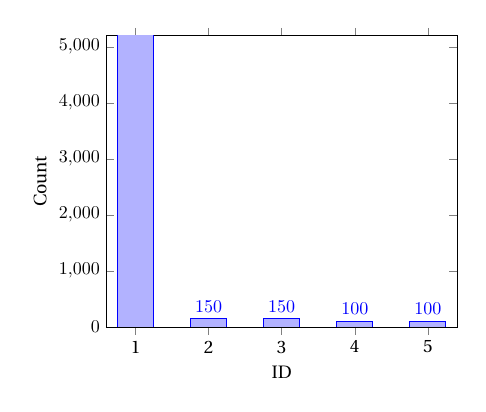
\begin{tikzpicture}[scale=0.65]
				\begin{axis}[
					ybar,
					ymin=0, % The minimum value on the y-axis.
					ymax=5200, % Adjust the maximum value according to your needs.
					symbolic x coords={1,2,3,4,5}, % X-axis coordinates.
					xtick=data, % Define ticks on the x-axis based on data points.
					nodes near coords, % Place nodes near the coordinates.
					nodes near coords align={vertical}, % Align the nodes vertically.
					xlabel={ID}, % Label for the x-axis.
					ylabel={Count}, % Label for the y-axis.
					bar width=20pt, % The width of the bars.
				]
				\addplot coordinates {(1,50000) (2,150) (3,150) (4,100) (5,100)}; % Data points for the plot.
				\end{axis}
			\end{tikzpicture}
			\caption{Data Skewing Example: ID Frequency histogram} % Add your caption
    		\label{fig:ch_3_hive_skewness_histogram} % Optional: For referencing the figure in text
			\end{figure}
			\end{tcolorbox}
		\end{frame}
		\begin{frame}
			\frametitle{CREATE TABLE in Hive | continued}  
			\vspace{-0.5cm}		
			\begin{tcolorbox}[colback=white,colframe=black,title= Part 7: Data Skewing]	
				\vspace{-0.3cm}
				\begin{figure}
					\includegraphics[width=\textwidth,height=.7\textheight,keepaspectratio]{./Figures/chapter-03/dwh_hive-skweed_dt_mr_2.png}	
					\caption{Abstract Components of Apache Hive}
				\end{figure}
				\vspace{-0.3cm}
			\end{tcolorbox}
		\end{frame}		
		\begin{frame}
			\frametitle{CREATE TABLE in Hive | continued}  
			\vspace{-0.5cm}		
			\begin{tcolorbox}[colback=white,colframe=black,title= Part 7: Data Skewing]					
				\begin{figure}
					\includegraphics[width=\textwidth,height=.7\textheight,keepaspectratio]{./Figures/chapter-03/dwh_hive-skweed_dt_mr.png}	
					\caption{Abstract Components of Apache Hive}
				\end{figure}
			\end{tcolorbox}
		\end{frame}	
		
		\begin{frame}
			\frametitle{CREATE TABLE in Hive | continued}  
			\vspace{-0.5cm}		
			\begin{tcolorbox}[colback=white,colframe=black,title= Part 7: Data Skewing]	
				\begin{figure}
					\includegraphics[width=\textwidth,height=.6\textheight,keepaspectratio]{./Figures/chapter-03/dwh_hive-unskweed_dt.png}	
					\caption{Abstract Components of Apache Hive}
				\end{figure}
			\end{tcolorbox}
		\end{frame}
		\begin{frame}
			\frametitle{CREATE TABLE in Hive | continued}  
			\vspace{-0.5cm}		
			\begin{tcolorbox}[colback=white,colframe=black,title= Part 7: Data Skewing]	
				\begin{figure}
					\includegraphics[width=\textwidth,height=.7\textheight,keepaspectratio]{./Figures/chapter-03/dwh_hive-unskweed_dt_mr.png}	
					\caption{Abstract Components of Apache Hive}
				\end{figure}
			\end{tcolorbox}
		\end{frame}	
		
		\begin{frame}{CREATE TABLE in Hive | continued}
			\begin{tcolorbox}[colback=white,colframe=black,title= Part 8: Table Location]
				\small
				\begin{itemize}
			  		\item \textbf{Resolving Skewness with Hive's \texttt{SKEWED BY} }
			  		\begin{itemize}
						\item When a table is created in Hive, you can specify certain columns as \texttt{'SKEWED BY'} to improve the distribution of work during a join operation. This allows Hive to partition the data more effectively.
			  		\end{itemize}
				\end{itemize}
			\end{tcolorbox}	
		\end{frame}
	
 \begin{frame}{CREATE TABLE in Hive | continued}
	\begin{tcolorbox}[colback=white,colframe=black,title= Part 8: Table Location]
		\small
		\begin{itemize}
			\item \texttt{[LOCATION hdfs\_path]}
			\begin{itemize}
				\item Sets the HDFS directory where table data will be stored.
			\end{itemize}
		\end{itemize}
	\end{tcolorbox}	
\end{frame}
  
  \begin{frame}{CREATE TABLE in Hive | continued}
	\begin{tcolorbox}[colback=white,colframe=black,title= Part 9: Table Properties]
		\small
	\begin{itemize}
	  \item \texttt{[TBLPROPERTIES (property\_name=property\_value, ...)]}
	  \begin{itemize}
		\item Sets table-level properties.
	  \end{itemize}
	\end{itemize}
	\end{tcolorbox}
  \end{frame}
  
  \begin{frame}{CREATE TABLE in Hive | continued}
	\begin{tcolorbox}[colback=white,colframe=black,title= Part 10: CTAS]
		\small
	\begin{itemize}
	  \item \texttt{[AS select\_statement]}
	  \begin{itemize}
		\item Populates the table using the result set of a SELECT statement.
	  \end{itemize}
	\end{itemize}
	\end{tcolorbox}
  \end{frame}
   












































%%%%%%%%%%%%%%%%%%%%%%%%%%%%%%%%%%%%%%%%%%%%%%%%%%%%%%
\subsubsection{Query Execution Plan}
\begin{frame}
	\frametitle{Query Execution Plan}
	\framesubtitle{Overview}
	
	\begin{itemize}
	  \item The Hive driver is responsible for translating SQL statements into an execution plan for the target execution engine.
	  \item The process involves several key steps:
		\begin{enumerate}
		  \item The parser parses the SQL statement and generates an Abstract Syntax Tree (AST) representing logical operations like SELECTs, JOINs, UNIONs, groupings, and more.
		  \item The planner retrieves table metadata from the Hive Metastore, including HDFS file locations, storage formats, row counts, etc.
		  \item The query optimizer utilizes the AST and table metadata to produce a physical operation tree known as the execution plan, defining the physical operations needed to retrieve data, such as nested loop joins, sort-merge joins, hash joins, index joins, and more.
		\end{enumerate}

	\end{itemize}
	
	\end{frame}
	
	\begin{frame}
	\frametitle{Query Execution Plan}
	\framesubtitle{Impact on Performance}
	
	\begin{itemize}
	\item The execution plan determines the tasks executed on the Hadoop cluster and significantly impacts performance in data analytics systems like Hive.
	  \item The execution plan generated by the query optimizer has a substantial impact on performance.
	  \item Differences in the execution plan can result in significant variations in execution time, ranging from seconds to hours.
	  \item An optimal execution plan is crucial for efficient query processing in Hive.
	\end{itemize}
	
	\end{frame}
	
	\begin{frame}
	\frametitle{Query Execution Plan}
	\framesubtitle{Cost-Based Optimization (CBO)}
	
	\begin{itemize}
	  \item The Cost-Based Optimization (CBO) plays a pivotal role in enhancing the execution plan.
	  \item CBO leverages table statistics to make informed decisions regarding the performance costs associated with each potential execution plan.
	  \item This intelligent optimization ensures that the Hive driver produces an optimal execution plan, improving query performance.
	\end{itemize}
	
	\end{frame}
\subsubsection{Cost-Based Optimization}
%%%%%%%%%%%%%%%%%%%%%%%%%%%%%%%%%%%%%%%%%%%%%%%%%%%%%%%%%%%%%%%%%%%%%%%%%%%


%%%%%%%%%%%%%%%%%%%%%%%%%%%%%%%%%%%%%%%%%%%%%%%%%%%%%%
\subsubsection{Hive Schema and Data Storage}
\begin{frame}{Hive Schema and Data Storage}
	\begin{itemize}
		\item Hive queries operate on tables, similar to RDBMS.
		\begin{itemize}
			\item A table corresponds to a directory in storage (HDFS, S3, GCS, or Azure).
			\item Each table comprises one or more files.
			\item Every table is associated with a specific file format.
			\item Hive stores table structure and location in the metadata store (RDBMS).
			\item Hive supports various file formats, such as Parquet, ORC, and Text.
		\end{itemize}
	\end{itemize}
\end{frame}

\begin{frame}{Hive Schema and Data Storage (Continued)}
	\begin{itemize}
		\item Hive queries reference the metastore to access table location and structure.
		\item While queries interact with the file system, metadata is stored in the RDBMS.
	\end{itemize}
\end{frame}
%%%%%%%%%%%%%%%%%%%%%%%%%%%%%%%%%%%%%%%%%%%%%%%%%%%%%%%%%%%%%%%%%%%%%%%%%%%
\subsection{Further Readings and Assignment}

%%% Local Variables:
%%% mode: latex
%%% TeX-master: "../main"
% !TeX root = ../main.tex
%%% TeX-engine: xetex
%%% End:
%    \section{Functional Programming}
\subsection{Why functional programming commonly used in distributed systems?}
\subsection{Introduction to Scala}
\subsection{Further Readings and Assignment}
%    \section{Spark Framework}

\subsection{Spark Philosophy towards the Engine and the Programming languages}

%\subsubsection{Introduction to Spark}
%%%%%%%%%%%%%%%%%%%%%%%%%%%%%%%%%%%%%%%%%%%%%%%%%%%%%%%%%%%%%%%%%%%%%%%%%%%
\begin{frame}
\frametitle{\secname : \subsecname}
\begin{itemize}[<+->]
	\item Any Big Data solution working based distributed systems.
	\item What is distributed systems in brief?
\end{itemize}
\end{frame}



\subsection{Spark Basics}


%\subsubsection{Introduction to Spark}
%%%%%%%%%%%%%%%%%%%%%%%%%%%%%%%%%%%%%%%%%%%%%%%%%%%%%%%%%%%%%%%%%%%%%%%%%%%
\begin{frame}
  \frametitle{\secname : \subsecname}
	\begin{itemize}[<+->]
		\item Any Big Data solution working based distributed systems.
		\item What is distributed systems in brief?
	\end{itemize}
\end{frame}

%%%%%%%%%%%%%%%%%%%%%%%%%%%%%%%%%%%%%%%%%%%%%%%%%%%%%%%%%%%%%%%%%%%%%%%%%%%
%\subsubsection{Map-Reduce using Spark}
\begin{frame}
  \frametitle{\subsecname}
	\begin{itemize}[<+->]
		\item Any Big Data solution working based distributed systems.
		\item What is distributed systems in brief?
	\end{itemize}
\end{frame}

%%%%%%%%%%%%%%%%%%%%%%%%%%%%%%%%%%%%%%%%%%%%%%%%%%%%%%%%%%%%%%%%%%%%%%%%%%%
\subsection{Spark Programming using RDDs}
\subsubsection{Spark RDD}

\begin{frame}
  \frametitle{\subsecname}
	\begin{itemize}[<+->]
		\item Any Big Data solution working based distributed systems.
		\item What is distributed systems in brief?
	\end{itemize}
\end{frame}
%%%%%%%%%%%%%%%%%%%%%%%%%%%%%%%%%%%%%%%%%%%%%%%%%%%%%%%%%%%%%%%%%%%%%%%%%%%

\subsubsection{Spark Working With Key/Value Pairs}

\begin{frame}
  \frametitle{\subsecname}
	\begin{itemize}[<+->]
		\item Any Big Data solution working based distributed systems.
		\item What is distributed systems in brief?
	\end{itemize}
\end{frame}

%%%%%%%%%%%%%%%%%%%%%%%%%%%%%%%%%%%%%%%%%%%%%%%%%%%%%%%%%%%%%%%%%%%%%%%%%%%

%\subsubsection{Why we need RDD in Real World Applications}

\begin{frame}
  \frametitle{\subsecname}
	\begin{itemize}[<+->]
		\item Any Big Data solution working based distributed systems.
		\item What is distributed systems in brief?
	\end{itemize}
\end{frame}


%%%%%%%%%%%%%%%%%%%%%%%%%%%%%%%%%%%%%%%%%%%%%%%%%%%%%%%%%%%%%%%%%%%%%%%%%%%
\subsection{Spark Datasets/Dataframe}

%\subsubsection{Introduction to Datasets/Dataframe}

\begin{frame}
  \frametitle{\subsecname}
	\begin{itemize}[<+->]
		\item Any Big Data solution working based distributed systems.
		\item What is distributed systems in brief?
	\end{itemize}
\end{frame}


%%%%%%%%%%%%%%%%%%%%%%%%%%%%%%%%%%%%%%%%%%%%%%%%%%%%%%%%%%%%%%%%%%%%%%%%%%%

\subsubsection{Spark SQL}
\begin{frame}
  \frametitle{\subsecname}
	\begin{itemize}[<+->]
		\item Any Big Data solution working based distributed systems.
		\item What is distributed systems in brief?
	\end{itemize}
\end{frame}

%%%%%%%%%%%%%%%%%%%%%%%%%%%%%%%%%%%%%%%%%%%%%%%%%%%%%%%%%%%%%%%%%%%%%%%%%%%

\subsubsection{Dataframes/Datasets vs. RDDs}

\begin{frame}
  \frametitle{\subsecname}
	\begin{itemize}[<+->]
		\item Any Big Data solution working based distributed systems.
		\item What is distributed systems in brief?
	\end{itemize}
\end{frame}

%%%%%%%%%%%%%%%%%%%%%%%%%%%%%%%%%%%%%%%%%%%%%%%%%%%%%%%%%%%%%%%%%%%%%%%%%%%
\subsection{Spark on Production}

%\subsubsection{Go Production Part 1}
\begin{frame}
  \frametitle{\subsecname}
	\begin{itemize}[<+->]
		\item Any Big Data solution working based distributed systems.
		\item What is distributed systems in brief?
	\end{itemize}
\end{frame}

%%%%%%%%%%%%%%%%%%%%%%%%%%%%%%%%%%%%%%%%%%%%%%%%%%%%%%%%%%%%%%%%%%%%%%%%%%%
%\subsubsection{Go Production Part 2}

\begin{frame}
  \frametitle{\subsecname}
	\begin{itemize}[<+->]
		\item Any Big Data solution working based distributed systems.
		\item What is distributed systems in brief?
	\end{itemize}
\end{frame}


%%%%%%%%%%%%%%%%%%%%%%%%%%%%%%%%%%%%%%%%%%%%%%%%%%%%%%%%%%%%%%%%%%%%%%%%%%%
\subsection{Spark For Batch Processing}
%\subsubsection{ETL pipeline End-to-End into Spark}

\begin{frame}
  \frametitle{\subsecname}
	\begin{itemize}[<+->]
		\item Any Big Data solution working based distributed systems.
		\item What is distributed systems in brief?
	\end{itemize}
\end{frame}

%%%%%%%%%%%%%%%%%%%%%%%%%%%%%%%%%%%%%%%%%%%%%%%%%%%%%%%%%%%%%%%%%%%%%%%%%%%


%%%%%%%%%%%%%%%%%%%%%%%%%%%%%%%%%%%%%%%%%%%%%%%%%%%%%%%%%%%%%%%%%%%%%%%%%%%
\subsection{Building custom input and output connector using Spark}
%\subsubsection{ETL pipeline End-to-End into Spark}

\begin{frame}
\frametitle{\subsecname}
\begin{itemize}[<+->]
	\item Any Big Data solution working based distributed systems.
	\item What is distributed systems in brief?
\end{itemize}
\end{frame}

%%%%%%%%%%%%%%%%%%%%%%%%%%%%%%%%%%%%%%%%%%%%%%%%%%%%%%%%%%%%%%%%%%%%%%%%%%%


%%%%%%%%%%%%%%%%%%%%%%%%%%%%%%%%%%%%%%%%%%%%%%%%%%%%%%%%%%%%%%%%%%%%%%%%%%%
\subsection{Spark Streaming}

%\subsubsection{Introduction to Spark Streaming}

\begin{frame}
  \frametitle{\subsecname}
	\begin{itemize}[<+->]
		\item Any Big Data solution working based distributed systems.
		\item What is distributed systems in brief?
	\end{itemize}
\end{frame}

%%%%%%%%%%%%%%%%%%%%%%%%%%%%%%%%%%%%%%%%%%%%%%%%%%%%%%%%%%%%%%%%%%%%%%%%%%%

%%%%%%%%%%%%%%%%%%%%%%%%%%%%%%%%%%%%%%%%%%%%%%%%%%%%%%%%%%%%%%%%%%%%%%%%%%%
%\subsubsection{Spark Streaming with Kafka}

\begin{frame}
  \frametitle{\subsecname}
	\begin{itemize}[<+->]
		\item Any Big Data solution working based distributed systems.
		\item What is distributed systems in brief?
	\end{itemize}
\end{frame}

%%%%%%%%%%%%%%%%%%%%%%%%%%%%%%%%%%%%%%%%%%%%%%%%%%%%%%%%%%%%%%%%%%%%%%%%%%%


%%%%%%%%%%%%%%%%%%%%%%%%%%%%%%%%%%%%%%%%%%%%%%%%%%%%%%%%%%%%%%%%%%%%%%%%%%%
%\subsubsection{Spark Structure Streaming}

\begin{frame}
  \frametitle{\subsecname}
	\begin{itemize}[<+->]
		\item Any Big Data solution working based distributed systems.
		\item What is distributed systems in brief?
	\end{itemize}
\end{frame}

%%%%%%%%%%%%%%%%%%%%%%%%%%%%%%%%%%%%%%%%%%%%%%%%%%%%%%%%%%%%%%%%%%%%%%%%%%%


%%%%%%%%%%%%%%%%%%%%%%%%%%%%%%%%%%%%%%%%%%%%%%%%%%%%%%%%%%%%%%%%%%%%%%%%%%%
%\subsubsection{Spark Streaming Applications}

\begin{frame}
  \frametitle{\subsecname}
	\begin{itemize}[<+->]
		\item Any Big Data solution working based distributed systems.
		\item What is distributed systems in brief?
	\end{itemize}
\end{frame}

%%%%%%%%%%%%%%%%%%%%%%%%%%%%%%%%%%%%%%%%%%%%%%%%%%%%%%%%%%%%%%%%%%%%%%%%%%%

\subsection{Spark using other Programming Languages}

%%%%%%%%%%%%%%%%%%%%%%%%%%%%%%%%%%%%%%%%%%%%%%%%%%%%%%%%%%%%%%%%%%%%%%%%%%%
\subsubsection{PySpsark for Python Geeks}

\begin{frame}
  \frametitle{\subsecname}
	\begin{itemize}[<+->]
		\item Any Big Data solution working based distributed systems.
		\item What is distributed systems in brief?
	\end{itemize}
\end{frame}

%%%%%%%%%%%%%%%%%%%%%%%%%%%%%%%%%%%%%%%%%%%%%%%%%%%%%%%%%%%%%%%%%%%%%%%%%%%
%\subsubsection{PySpsark Utilizing Python Features}

\begin{frame}
  \frametitle{\subsecname}
	\begin{itemize}[<+->]
		\item Any Big Data solution working based distributed systems.
		\item What is distributed systems in brief?
	\end{itemize}
\end{frame}

%%%%%%%%%%%%%%%%%%%%%%%%%%%%%%%%%%%%%%%%%%%%%%%%%%%%%%%%%%%%%%%%%%%%%%%%%%%
\subsubsection{RSpark for R Geeks}

\begin{frame}
  \frametitle{\subsecname}
	\begin{itemize}[<+->]
		\item Any Big Data solution working based distributed systems.
		\item What is distributed systems in brief?
	\end{itemize}
\end{frame}

%%%%%%%%%%%%%%%%%%%%%%%%%%%%%%%%%%%%%%%%%%%%%%%%%%%%%%%%%%%%%%%%%%%%%%%%%%%

\subsection{Spark For Data Scientist}

%%%%%%%%%%%%%%%%%%%%%%%%%%%%%%%%%%%%%%%%%%%%%%%%%%%%%%%%%%%%%%%%%%%%%%%%%%%


%\subsubsection{Data Analysis using Spark}

\begin{frame}
  \frametitle{\subsecname}
	\begin{itemize}[<+->]
		\item Any Big Data solution working based distributed systems.
		\item What is distributed systems in brief?
	\end{itemize}
\end{frame}

%%%%%%%%%%%%%%%%%%%%%%%%%%%%%%%%%%%%%%%%%%%%%%%%%%%%%%%%%%%%%%%%%%%%%%%%%%%
%\subsubsection{Machine Leaning using Spark }

\begin{frame}
  \frametitle{\subsecname}
	\begin{itemize}[<+->]
		\item Any Big Data solution working based distributed systems.
		\item What is distributed systems in brief?
	\end{itemize}
\end{frame}

%%%%%%%%%%%%%%%%%%%%%%%%%%%%%%%%%%%%%%%%%%%%%%%%%%%%%%%%%%%%%%%%%%%%%%%%%%%

%%%%%%%%%%%%%%%%%%%%%%%%%%%%%%%%%%%%%%%%%%%%%%%%%%%%%%%%%%%%%%%%%%%%%%%%%%%
%\subsubsection{Deep Learning using Spark}

\begin{frame}
  \frametitle{\subsecname}
	\begin{itemize}[<+->]
		\item Any Big Data solution working based distributed systems.
		\item What is distributed systems in brief?
	\end{itemize}
\end{frame}

%%%%%%%%%%%%%%%%%%%%%%%%%%%%%%%%%%%%%%%%%%%%%%%%%%%%%%%%%%%%%%%%%%%%%%%%%%%

\subsection{Spark Graph Dataframe/Graphx}
%%%%%%%%%%%%%%%%%%%%%%%%%%%%%%%%%%%%%%%%%%%%%%%%%%%%%%%%%%%%%%%%%%%%%%%%%%%
%\subsubsection{Introduction to Spark Graph Dataframe/GraphX}

\begin{frame}
  \frametitle{\subsecname}
	\begin{itemize}[<+->]
		\item Any Big Data solution working based distributed systems.
		\item What is distributed systems in brief?
	\end{itemize}
\end{frame}

%%%%%%%%%%%%%%%%%%%%%%%%%%%%%%%%%%%%%%%%%%%%%%%%%%%%%%%%%%%%%%%%%%%%%%%%%%%
%\subsubsection{Graph Applications using Spark}

\begin{frame}
  \frametitle{\subsecname}
	\begin{itemize}[<+->]
		\item Any Big Data solution working based distributed systems.
		\item What is distributed systems in brief?
	\end{itemize}
\end{frame}


%%%%%%%%%%%%%%%%%%%%%%%%%%%%%%%%%%%%%%%%%%%%%%%%%%%%%%%%%%%%%%%%%%%%%%%%%%%

\subsection{Tuning your Spark Jobs}

%%%%%%%%%%%%%%%%%%%%%%%%%%%%%%%%%%%%%%%%%%%%%%%%%%%%%%%%%%%%%%%%%%%%%%%%%%%
%\subsubsection{Tuning Spark Jobs Part 1}

\begin{frame}
  \frametitle{\subsecname}
	\begin{itemize}[<+->]
		\item Any Big Data solution working based distributed systems.
		\item What is distributed systems in brief?
	\end{itemize}
\end{frame}

%%%%%%%%%%%%%%%%%%%%%%%%%%%%%%%%%%%%%%%%%%%%%%%%%%%%%%%%%%%%%%%%%%%%%%%%%%%
%\subsubsection{Tuning Spark Jobs Part 2}

\begin{frame}
  \frametitle{\subsecname}
	\begin{itemize}[<+->]
		\item Any Big Data solution working based distributed systems.
		\item What is distributed systems in brief?
	\end{itemize}
\end{frame}

%Shared Variables
%Catalyst. 
%Tungsten
%SQL Joins
\subsection{Further Readings and Assignment}
%    \section{Real World Applications}
%\subsection{Problems in Big Data Projects}
\subsection{Big Data Development Life Cycle}
\subsection{Template Concept for Data Engineering}
\subsubsection{Template for ETL Application}
\subsubsection{Template for QA}
\subsubsection{Template for Streaming Applications}
\subsubsection{Template for Machine Learning Applications}
\subsection{Further Readings and Assignment}

%%%%%%%%%%%%%%%%%%%%%%%%%%%%%%%%%%%%%%%%%%%%%%%%%%%%%%%%%%%%%%%%%%%%%%%%%%%
%%% Local Variables:
%%% mode: latex
%%% TeX-master: "../main"
% !TeX root = ../main.tex
%%% TeX-engine: xetex
%%% End:
%    \section{Massaging Systems}
%\subsection{Problems in Big Data Projects}
\subsection{Motivation}
\subsection{Massaging Systems Architecture}
\subsection{JMS as an example}
\subsection{Introduction to Kafka}
\subsubsection{Kafka Architecture}
\subsubsection{Kafka Topics}
\subsubsection{Partitions}
\subsubsection{Kafka Producers}
\subsubsection{Kafka Consumers}
\subsubsection{Kafka Connector}
\subsubsection{Kafka Custom Connectors}
\subsubsection{Kafka Configuration}
\subsubsection{Kafka Configuration Optimizations}
\subsubsection{Kafka Operations}
\subsubsection{Kafka Integration with Enterprise tools}% Spring integration
\subsection{Further Readings and Assignment}
%%%%%%%%%%%%%%%%%%%%%%%%%%%%%%%%%%%%%%%%%%%%%%%%%%%%%%%%%%%%%%%%%%%%%%%%%%%
%%% Local Variables:
%%% mode: latex
%%% TeX-master: "../main"
% !TeX root = ../main.tex
%%% TeX-engine: xetex
%%% End:
%    \section{Data Orchestration}
\subsection{Motivation}
\subsection{Enterprise vs Open source tools}
\subsubsection{Open source tools (Oozie as an Example)}
\subsubsection{Enterprise source tools}
\subsubsection{How to choose the right tool?}
\subsection{Further Readings and Assignment}
%    \section{NOSQL}
\subsection{Introduction to NoSQL Databases.}
\subsection{Cassandra}
\subsubsection{Why Cassandra?}
\subsubsection{Introducing Cassandra}
\subsubsection{The Cassandra Data Model}
\subsubsection{Architecture}
\subsubsection{Reading and Writing Data}
\subsubsection{Integrating Hadoop}
\subsection{Assignment and Homework}
%    \section{Elastic}

\subsection{Assignment and Homework}
%    \section{Data Architecture Design}
\subsection{Further Readings and Assignment}
%    %%%%%%%%%%%%%%%%%%%%%%%%%%%%%%%%%%%%%%%%%%%%%%%%%%%%%%%%%%%%%%%%%%%%%%%%%%%
%\begin{appendices}
\section{Appendix}
          
\subsection{Appendix A- Shell Programming}  
%%%%%%%%%%%%%%%%%%%%%%%%%%%%%%%%%%%%%%%%%%%%%%%%%%%%%%%%%%%%%%%%%%%%%%%%%%%
\begin{frame}
\frametitle{Appendix A- Shell Programming}
\begin{itemize}[<+->]
	\item Any Big Data solution working based distributed systems.
	\item What is distributed systems in brief?
\end{itemize}
\end{frame}

%%%%%%%%%%%%%%%%%%%%%%%%%%%%%%%%%%%%%%%%%%%%%%%%%%%%%%%%%%%%%%%%%%%%%%%%%%%
\subsection{Appendix B- Java Programming}   
%%%%%%%%%%%%%%%%%%%%%%%%%%%%%%%%%%%%%%%%%%%%%%%%%%%%%%%%%%%%%%%%%%%%%%%%%%%
\begin{frame}
\frametitle{Appendix B- Java Programming}
\begin{itemize}[<+->]
	\item Any Big Data solution working based distributed systems.
	\item What is distributed systems in brief?
\end{itemize}
\end{frame}

%%%%%%%%%%%%%%%%%%%%%%%%%%%%%%%%%%%%%%%%%%%%%%%%%%%%%%%%%%%%%%%%%%%%%%%%%%%

\subsection{Appendix C- Scala Programming}  
%%%%%%%%%%%%%%%%%%%%%%%%%%%%%%%%%%%%%%%%%%%%%%%%%%%%%%%%%%%%%%%%%%%%%%%%%%%
\begin{frame}
\frametitle{Appendix C- Scala Programming}
\begin{itemize}[<+->]
	\item Any Big Data solution working based distributed systems.
	\item What is distributed systems in brief?
\end{itemize}
\end{frame}

%%%%%%%%%%%%%%%%%%%%%%%%%%%%%%%%%%%%%%%%%%%%%%%%%%%%%%%%%%%%%%%%%%%%%%%%%%%

\subsection{Appendix D- SQL Programming}
%%%%%%%%%%%%%%%%%%%%%%%%%%%%%%%%%%%%%%%%%%%%%%%%%%%%%%%%%%%%%%%%%%%%%%%%%%%
\begin{frame}
\frametitle{Appendix D- SQL Programming}
\begin{itemize}[<+->]
	\item Any Big Data solution working based distributed systems.
	\item What is distributed systems in brief?
\end{itemize}
\end{frame}

%%%%%%%%%%%%%%%%%%%%%%%%%%%%%%%%%%%%%%%%%%%%%%%%%%%%%%%%%%%%%%%%%%%%%%%%%%%

\subsection{Appendix E- Oozie Programming}
%%%%%%%%%%%%%%%%%%%%%%%%%%%%%%%%%%%%%%%%%%%%%%%%%%%%%%%%%%%%%%%%%%%%%%%%%%%
\begin{frame}
\frametitle{Appendix E- Oozie Programming}
\begin{itemize}[<+->]
	\item Any Big Data solution working based distributed systems.
	\item What is distributed systems in brief?
\end{itemize}
\end{frame}

%%%%%%%%%%%%%%%%%%%%%%%%%%%%%%%%%%%%%%%%%%%%%%%%%%%%%%%%%%%%%%%%%%%%%%%%%%%

\subsection{Appendix F- DWH Concepts}
%%%%%%%%%%%%%%%%%%%%%%%%%%%%%%%%%%%%%%%%%%%%%%%%%%%%%%%%%%%%%%%%%%%%%%%%%%%
\begin{frame}
\frametitle{Appendix F- DWH Concepts}
\begin{itemize}[<+->]
	\item Any Big Data solution working based distributed systems.
	\item What is distributed systems in brief?
\end{itemize}
\end{frame}

%%%%%%%%%%%%%%%%%%%%%%%%%%%%%%%%%%%%%%%%%%%%%%%%%%%%%%%%%%%%%%%%%%%%%%%%%%%

\subsection{Appendix G- Machine Learning Concepts Data Engineers}
%%%%%%%%%%%%%%%%%%%%%%%%%%%%%%%%%%%%%%%%%%%%%%%%%%%%%%%%%%%%%%%%%%%%%%%%%%%
\begin{frame}
\frametitle{Appendix G- Machine Learning Concepts Data Engineers}
\begin{itemize}[<+->]
	\item Any Big Data solution working based distributed systems.
	\item What is distributed systems in brief?
\end{itemize}
\end{frame}

%%%%%%%%%%%%%%%%%%%%%%%%%%%%%%%%%%%%%%%%%%%%%%%%%%%%%%%%%%%%%%%%%%%%%%%%%%%

\subsection{Appendix H- Docker for Data Engineers}
%%%%%%%%%%%%%%%%%%%%%%%%%%%%%%%%%%%%%%%%%%%%%%%%%%%%%%%%%%%%%%%%%%%%%%%%%%%
\begin{frame}
\frametitle{Appendix H- Docker for Data Engineers}
\begin{itemize}[<+->]
	\item Any Big Data solution working based distributed systems.
	\item What is distributed systems in brief?
\end{itemize}
\end{frame}

%%%%%%%%%%%%%%%%%%%%%%%%%%%%%%%%%%%%%%%%%%%%%%%%%%%%%%%%%%%%%%%%%%%%%%%%%%%


%%%%%%%%%%%%%%%%%%%%%%%%%%%%%%%%%%%%%%%%%%%%%%%%%%%%%%%%%%%%%%%%%%%%%%%%%%%
%%% Local Variables:
%%% mode: latex
%%% TeX-master: "../main"
%%% TeX-engine: xetex
%%% End:


%%%%%%%%%%%%%%%%%%%%%%%%%%%%%%%%%%%%%%%%%%%%%%%%%%%%%%

\begin{frame}[c]{ }
    \centering     
   
    \textcolor{offgreen}{ \large Thank you for watching!}
\end{frame}


\begin{frame}[c]{ }
    \centering 
    \textcolor{offyellow}{\large See you in the next video \Smiley{}}
\end{frame}
    %%%%%%%%%%%%%%%%%%%%%%%%%%%%%%%%%%%%%%%%%%%%%%%%%%%%%%%%%%%%%%%%%%%%%%%%%%%%%%%%%%%%%%%
\end{document}

%%% Local Variables:
%%% mode: latex
%%% TeX-master: t
%%% TeX-engine: xetex
%%% End:
